\documentclass[10 pt]{article}
\usepackage{style}

\title{\Large \bfseries {Concentration of Contractive Stochastic Approximation: Additive and Multiplicative Noise}}
\author{\normalsize Zaiwei Chen\textsuperscript{1,$*$} Siva Theja Maguluri\textsuperscript{2}, and Martin Zubeldia\textsuperscript{3,$*$}\\
{\footnotesize
\textsuperscript{1}Caltech CMS, \href{mailto:zchen458@caltech.edu}{\textit{zchen458@caltech.edu}}}
{\footnotesize\textsuperscript{2}Georgia Tech ISyE, \href{mailto:siva.theja@gatech.edu}{\textit{siva.theja@gatech.edu}}}\\
{\footnotesize\textsuperscript{3}University of Minnesota ISyE, \href{mailto:zubeldia@umn.edu}{\textit{zubeldia@umn.edu}}}
}
\setcounter{tocdepth}{2} 
\def\checkmark{\tikz\fill[scale=0.4](0,.35) -- (.25,0) -- (1,.7) -- (.25,.15) -- cycle;}

\date{\vspace{-0.3 in}}

\begin{document}
\maketitle

\pagestyle{fancy}
\fancyhf{} 
\fancyhead[R]{\thepage}

\begin{abstract}
\blfootnote{$^*$ Equal contribution.}In this work, we study the concentration behavior of a stochastic approximation (SA) algorithm under a contractive operator with respect to an arbitrary norm. We consider two settings where the iterates are potentially unbounded: (1) bounded multiplicative noise, and (2) additive sub-Gaussian noise. We obtain maximal concentration inequalities on the convergence errors, and show that these errors have sub-Gaussian tails in the additive noise setting, and super-polynomial tails (faster than polynomial decay) in the multiplicative noise setting. In addition, we provide an impossibility result showing that it is in general not possible to achieve sub-exponential tails for SA with multiplicative noise. To establish these results, we develop a novel \textit{bootstrapping argument} that involves bounding the moment generating function of the generalized Moreau envelope of the error and the construction of an exponential supermartingale to enable using Ville's maximal inequality.

To demonstrate the applicability of our theoretical results, we use them to provide maximal concentration bounds for a large class of reinforcement learning algorithms, including but not limited to on-policy TD-learning with linear function approximation, off-policy TD-learning with generalized importance sampling factors, and $Q$-learning. To the best of our knowledge, super-polynomial concentration bounds for off-policy TD-learning have not been established in the literature due to the challenge of handling the combination of unbounded iterates and multiplicative noise. 
\end{abstract}




\section{Introduction}\label{sec:intro}



Stochastic approximation (SA) \citep{robbins1951stochastic} is the underlying workhorse for modern large-scale optimization and machine learning, which have achieved great successes in solving many practical problems \citep{kober2013reinforcement,silver2017mastering,jumper2021highly}. In this work, we consider an SA algorithm of the form
\begin{equation}\label{eq:recursion}
x_{k+1} = x_k + \alpha_k(F(x_k,Y_k) - x_k),
\end{equation}
where $Y_k\in\mathcal{Y}$ is a random variable representing the noise, $F:\mathbb{R}^d\times\mathcal{Y}\mapsto\mathbb{R}^d$ is a (possibly nonlinear) operator, and $\alpha_k>0$ is the stepsize. We assume that the expectation of the operator $F(\cdot,Y_k)$ with respect to the noise, denoted by $\bar{F}(\cdot)$, is a contraction mapping with respect to some arbitrary norm $\|\cdot\|_c$. See Section \ref{sec:sa} for the formal description of the SA model.

Algorithm (\ref{eq:recursion}) covers many existing popular algorithms as its special cases. For example, when $F(x_k,Y_k)=-\nabla J(x_k)+x_k+Y_k$ for some objective function $J(\cdot)$, Algorithm (\ref{eq:recursion}) is the stochastic gradient descent (SGD) algorithm used to minimize $J(\cdot)$ \citep{lan2020first}. In the context of reinforcement learning (RL), popular algorithms such as $Q$-learning and variants of TD-learning can all be modeled in the form of Algorithm (\ref{eq:recursion}) \citep{bertsekas1996neuro}, where the expected operator $\bar{F}(\cdot)$ is closely related to the Bellman operator. Due to wide applications of Algorithm (\ref{eq:recursion}), theoretically understanding the evolution of $\{x_k\}$ is of fundamental interest.

Early literature on SA focused on the asymptotic convergence, i.e., the behavior of $x_k$ as $k$ goes to infinity \citep{robbins1951stochastic,borkar2009stochastic,tsitsiklis1994asynchronous,kushner2012stochastic}. In recent years, finite-sample analysis has received considerable attention \citep{bhandari2018finite,srikant2019finite,chen2020finite}. In finite-sample analysis, the goal is to bound the error between the stochastic iterate $x_k$ and its limit $x^*$ (provided that the asymptotic convergence was already established) as a function of the number of iterations $k$, and to study its decay rate. Finite-sample analysis not only provides theoretical understanding of the evolution of SA algorithms, but can also be used as a guideline in implementation. 

Due to the stochastic nature of the iterates, there are multiple ways of measuring the distance between the iterates and the limit point. One natural way is to use the mean-square distance $\mathbb{E}[\|x_k-x^*\|_c^2]$, which has been extensively studied in the literature \citep{srikant2019finite,bhandari2018finite,chen2019finitesample,chen2020finite,wainwright2019high}. Another popular way is to use the probability that $\|x_k-x^*\|_c\leq \epsilon$ for some $\epsilon>0$. A bound on this probability is called a ``high probability bound'', and is sometimes preferable over a mean-square bound as it not only provides the convergence rate, but also the confidence level. However, high probability bounds are in general more challenging to establish. For example, consider the convergence rate of the law of large numbers\footnote{The average of a sequence of random variables $\frac{1}{k}\sum_{i=0}^{k-1}Y_k$ can be computed in an iterative manner as $x_{k+1}=x_k+\frac{1}{k+1}(-x_k+Y_k)$ with $x_0=\bm{0}$, which is clearly a special case of Algorithm (\ref{eq:recursion}).}. The establishment of the $\mathcal{O}(1/k)$ mean-square bound is significantly easier than establishing exponential tail bounds such as Hoeffding's inequality, Chernoff bound, and Bernstein's inequality, etc.

To establish high probability bounds of Algorithm (\ref{eq:recursion}), the operator $F(\cdot,\cdot)$ and noise sequence $\{Y_k\}$ play important roles in the analysis. Most of existing literature focus on the setting where the noise in the SA algorithm appears in an additive manner, and is a.s. bounded. To illustrate, consider linear SA of the form $x_{k+1}=x_k+\alpha_k(A(Y_k)x_k-b(Y_k))$, where $A:\mathcal{Y}\mapsto\mathbb{R}^{d\times d }$ and $b:\mathcal{Y}\mapsto\mathbb{R}^d$ are deterministic functions. When $A(Y_k)$ is not random (or equivalently $A(Y_k)=\mathbb{E}[A(Y_k)]$ a.s.), the noise is purely additive. For the multiplicative noise setting, which corresponds to $A(Y_k)$ being random, the analysis is much more challenging. Existing results either do not have super-polynomial tail bounds or require strong assumptions, such as $A(Y_k)$ being Hurwitz a.s. See Section \ref{subsec:literature} for a more detail literature review. In this work, we develop maximal super-polynomial concentration bounds for SA algorithms involving additive and/or multiplicative noise. In addition, we go beyond linear SA and consider more general contractive SA algorithms of the form (\ref{eq:recursion}), which covers linear SA as a special case as will be illustrated in Section \ref{sec:linearSA}. 

\subsection{Our Contributions}

The main contributions of this work are summarized in the following.

\paragraph{Multiplicative Noise Setting.} We establish a super-polynomial high probability bound under diminishing stepsizes of the form $\alpha_k=\alpha/(k+h)$. Importantly, our high probability bound provides a bound on the entire tail of the iterates, as our stepsizes do not depend on either the desired accuracy level $\epsilon$ or the confidence level $\delta$. Moreover, our bound is ``maximal'' in the sense that it is a bound on the concentration behavior of the entire trajectory of the iterates $\{x_k\}$. As a complement of the concentration bounds, we provide an impossibility result showing that concentration bounds with sub-exponential tails are in general not achievable. To our knowledge, this is the first maximal super-polynomial high probability bound for SA with multiplicative noise. Even for the simple setting of linear SA (with a random $A(Y_k)$ that is not a.s. Hurwitz), such concentration result is unknown in the literature.

\paragraph{Additive Noise Setting.} We also consider the case of purely additive noise. We allow the noise to be unbounded, albeit sub-Gaussian. In this case, we establish maximal high probability bounds (with exponentially small tail) for the SA algorithm when using either linearly diminishing stepsizes $\alpha_k=\alpha/(k+h)$ or polynomially diminishing stepsizes $\alpha_k=\alpha/(k+h)^z$ with $z\in (0,1)$. To our knowledge, except for the special case of SGD, such concentration results in the case of additive but unbounded noise are unknown in the literature.

\paragraph{Applications in RL.} The generality of our SA results enables us to study the concentration behavior of a large class of RL algorithms, a typical example of which is off-policy TD-learning. Note that off-policy TD involves multiplicative noise, and does not have uniformly bounded iterates. This makes establishing high probability bounds of off-policy TD-learning very challenging, and to the best of our knowledge, there are no such results in the literature. In addition to off-policy TD, we also establish maximal high probability bounds for on-policy TD-learning with linear function approximation and $Q$-learning.

\paragraph{Methodological Contributions.} To handle the multiplicative noise in the SA algorithm, we develop a novel proof technique involving (1) the establishment of a bound on a properly modified moment generating function (MGF) of the generalized Moreau envelope of the error, which serves as a potential/Lyapunov function in our approach, (2) the proper construction of an exponential supermartingale and the use of Ville's maximal inequality, and (3) a novel bootstrapping method used to overcome the potential unboundedness of the iterates. More details about the challenges and our technical contributions are presented in the next subsection.



\subsection{Challenges \& Our Techniques}\label{subsec:challenge}

We use SA under multiplicative noise as an example to present the challenges and our techniques. The analysis of SA with additive noise follows a similar approach. The main challenge of obtaining super-polynomial high probability bounds is due to the combination of \textit{unbounded iterates} and \textit{multiplicative noise}. While having unbounded iterates and multiplicative noise are not too problematic in isolation, the combination of both creates a setting where the variance of the noise is unbounded. In this case, since we allow the multiplicative noise to be large enough so that the ``noisy'' operator can be expansive with positive probability, the error can grow extremely fast with a significant probability. This creates a challenge that no approach in the literature can deal with in general. To overcome this challenge, we develop a novel bootstrapping argument. The high level ideas are presented in the following.

\paragraph{Initialization: Time-Varying Worst-Case Bounds.} While the iterates of SA with multiplicative noise are not uniformly bounded by a constant, we show that they do admit a time-varying a.s. bound. The behavior of such time-varying bound depends on the contraction effect in the expected operator and the expansive effect in the multiplicative noise. In general, the bound can be polynomially \textit{increasing} with time.

\paragraph{Bootstrapping: An Iterative Framework to Improve the Bound.} The key in the bootstrapping argument is to start with a non-decreasing sequence $\{T_k(\delta)\}_{k\geq 0}$ such that 
\begin{align*}
    \mathbb{P}(\|x_k-x^*\|_c^2\leq T_k(\delta),\forall\;k\geq 0)\geq 1-\delta,
\end{align*}
and obtain a sequence $\{T_k(\delta,\delta')\}_{k\geq 0}$, with $T_k(\delta,\delta')=\tilde{\mathcal{O}}(T_k(\delta)/k)$, such that 
\begin{align*}
    \mathbb{P}(\|x_i-x^*\|_c^2\leq T_k(\delta,\delta'),\forall\;k\geq 0)\geq 1-\delta-\delta'.
\end{align*}
This blueprint enables us to start with the time-varying worst-case bound for the error (which can be polynomially increasing) and iteratively improve it to obtain our super-polynomial concentration bound with the desired convergence rate. It will become clear from the proof that, for this bootstrapping argument to work, the fact that the bounds hold for all $k\geq 0$ is fundamental. To establish this blueprint, we develop a two-step Lyapunov argument.

\begin{itemize}
    \item {\bf Step 1: Recursive Bound on the Log-MGFs:} The first step is to obtain a recursive upper bound between the log-MGF of $\|x_{k+1}-x^*\|_c^2$ and that of $\|x_k-x^*\|_c^2$. Opening this recursion, we also obtain an outright bound on $\|x_k-x^*\|_c^2$ that only depends on $\|x_0-x^*\|_c^2$ and other model parameters. These bounds are valid for all $k\geq 0$, and give us a tight grasp on the effect of the noise on the error.
    \item {\bf Step 2: Exponential Supermartingale:} We construct a supermartingale $\{\overline{M}_k\}_{k\geq 0}$ of the form $\overline{M}_k=\exp(\|x_k-x^*\|_c^2 \alpha_k^{-1}T_k(\delta)^{-1}- C \sum_{i=0}^{k-1} \alpha_k ) $ and use Ville's maximal inequality to obtain a maximal bound on the iterates. In particular, this maximal bound states that $\|x_k-x^*\|_c^2$ is $\tilde{\mathcal{O}}(\alpha_k T_k(\delta))$ for all $k \geq 0$ with high probability. Since $\alpha_k=\mathcal{O}(1/k)$, the bootstrapping blueprint is established. 
    
    Note that on an aside, if the initial high probability bound $T_k(\delta)$ is a constant (which implies that the SA algorithm has bounded iterates, such as $Q$-learning), we only need to apply the bootstrapping argument once to get a maximal high probability bound of order $\mathcal{O}(1/k)$.
\end{itemize}





\subsection{Related Literature}\label{subsec:literature}

Due to the wide applications, there are extensive related literature on establishing concentration bounds of SA algorithms in the form of SGD, linear SA, and RL algorithms.

\subsubsection{Stochastic Gradient Descent}

There is a large body of work about exponential high probability bounds for SGD and its variants. In \cite{rakhlin2012,Hazan14}, the authors obtain exponential high probability bounds for non-smooth strongly convex functions, when the noise is conditionally unbiased and the iterates are in a compact set. This was later generalized for the case of sub-Gaussian noise and unbounded iterates in \cite{Harvey19}, making it one of the rare cases where exponential high probability bounds are obtained with unbounded noise. Exponential high probability bounds were also obtained for the ergodic mirror descent (under Markovian, conditionally biased noise with uniformly bounded variance) in \cite{duchi2012ergodic}, under the additional assumption that the iterates are in a compact set. 
More recently, polynomial high probability bounds have been obtained in \cite{heavySGD} for SGD on linear models when the noise is heavy-tailed. Finally, in \cite{telgarsky22}, the authors analyze mirror descent with constant stepsize, and i.i.d. noise with uniformly bounded variance that is a.s. bounded or sub-Gaussian. By choosing the constant stepsize appropriately, they obtain exponential high probability bounds in this setting.



\subsubsection{Linear Stochastic Approximation}
For linear SA, the first moment bounds for the $\ell_2$-norm of the error with constant stepsize were given in \cite{lakshminarayanan2018linear,srikant2019finite}. Based on these, one could obtain high probability bounds, albeit with polynomial tails instead of exponential ones.

To our knowledge, the strongest result on exponential high probability bounds for linear SA is given in \cite{dalal2018general}. There, the authors analyze a two-timescale linear SA with decreasing stepsizes, and with multiplicative, a.s. bounded, martingale-difference noise. In this setting, they obtain maximal exponential high probability bounds for all iterates large enough by choosing stepsizes that depend on both the runtime and the probability tolerance level. On the other hand, there is a line of work that focuses primarily on the product of random matrices, and then applies these results to linear SA. In \cite{durmus2021tight}, the authors consider an linear SA with constant stepsize, where the noise is Markovian and a.s. bounded. In this setting, they develop high probability bounds on the product of random matrices to obtain sub-exponential high probability bounds when the random matrices are almost surely Hurwitz, and polynomial high probability bounds when the random matrices are only Hurwitz in expectation. This was later extended to the case of Polyak-Ruppert averaged iterates in \cite{durmusAveraged,Mou20}.


\subsubsection{Reinforcement Learning}

In one of the earliest works about exponential high probability bounds in RL \citep{even2003learning}, the authors analyze synchronous $Q$-learning algorithm when the stepsizes are $\mathcal{O}(k^{-z})$, for $z\in(1/2,1)$. In this setting, they obtain exponential high probability bounds for all iterates large enough. In \cite{LSTD17}, the authors consider the LSTD algorithm (which includes a projection step onto a compact set), and obtain exponential high probability bounds for the $\ell_2$-norm of the error when the stepsizes are $\mathcal{O}(k^{-1})$. In \cite{dalal2018finite}, the authors analyze TD($0$) with linear function approximation, where the noise is assumed to be i.i.d. instead of Markovian. In that setting, they obtain maximal exponential high-probability bounds for the $\ell_2$-norm of the error in the last iterate, for iterates beyond some point that is of order $\log(1/\delta)$. Recently in \cite{li2020sample,li2021q}, the authors analyze the popular $Q$-learning algorithm with constant stepsize and uniformly bounded, Markovian, possibly conditionally biased noise. In this setting, given a runtime and a performance guarantee, they obtain exponential high probability bounds at the end of the runtime, provided that it is large enough.

\begin{table}[ht!]
\begin{center}
\begin{tabular}{ |c|c|c|c|c|c| } 
 \hline
 \rowcolor{Gray} Paper & Operator & \hspace{-2mm} \begin{tabular}{c} \!\!\!Unbounded\!\!\!\\iterates \end{tabular} \hspace{-2mm} & \hspace{-2mm} \begin{tabular}{c}\!\!No tuned\\stepsize\!\! \end{tabular} \hspace{-2mm} & \hspace{-2mm} \begin{tabular}{c}\!\!Mult.\\noise\!\! \end{tabular} \hspace{-2mm} & \hspace{-2mm} \begin{tabular}{c}For any\\ $k\geq 0$ \end{tabular} \hspace{-2mm} \\ 
 \hline\hline
 \cite{li2021q} & $Q$-learning & & & &  \\
 \hline
 \cite{even2003learning} & $Q$-learning & & \checkmark &  &  \\
 \hline
 \cite{qu2020finite} & $Q$-learning & & \checkmark &  & \checkmark \\
 \hline
 \cite{duchi2012ergodic} & EMD & & \checkmark & & \checkmark \\ 
 \hline
 \cite{LSTD17} & LSTD & & \checkmark & & \checkmark \\
 \hline
 \cite{thoppe2019concentration} & Any & & \checkmark & \checkmark * &  \\ 
 \hline
 \cite{chandak2022concentration} & Any & & \checkmark & \checkmark * &  \\ 
 \hline
 \cite{telgarsky22} & MD & \checkmark &  &  &  \\ 
 \hline
 \cite{infiniteDim22} & Any & \checkmark &  & \checkmark &  \\ 
 \hline
 \cite{dalal2018general} & Linear & \checkmark & & \checkmark  &  \\
 \hline
 \cite{rakhlin2012} & SGD & \checkmark & \checkmark & &  \\ 
 \hline
 \cite{dalal2018finite} & TD(0) & \checkmark & \checkmark & \checkmark & \\
 \hline
 \cite{durmus2021tight} & Linear & \checkmark & \checkmark & \checkmark * & \checkmark \\ 
 \hline
 \rowcolor{LightCyan} Theorem \ref{thm:multi}  & Any & \checkmark & \checkmark & \checkmark & \checkmark \\ 
 \hline
 \rowcolor{LightCyan} Theorem \ref{thm:additive} & Any & \checkmark & \checkmark &  & \checkmark \\ 
 \hline
\end{tabular}
\end{center}
\caption{Summary of previous work on high probability bounds for SA and its special cases. An asterisk indicates that the assumption only holds for constants small enough.}
\label{tab:summary}
\end{table}

\subsubsection{General Stochastic Approximation}
For general nonlinear SA under arbitrary norms and decreasing stepsizes, the authors of \cite{chen2020finite,chen2019finitesample} obtain bounds on the second moment of the error. These moment bounds can be used to obtain high probability bounds, albeit without exponential tails.

In \cite{thoppe2019concentration}, the authors consider an SA with decreasing stepsizes, and martingale-difference sub-exponential noise. In this setting, they obtain maximal exponential high probability bounds conditioned on the event that the iterates are close enough to the fixed point after some time. In follow-up work \cite{chandak2022concentration}, they assume that their noise is multiplicative, a.s. bounded, and Markovian. In this setting, they obtain maximal exponential high probability bounds without conditioning on an unknown event. However, their high probability bounds only hold for after some time, and both the bound and the probabilities depend on the unknown norm of the iterate after some time (which is random, with unknown distribution). 

In a separate line of work, in \cite{qu2020finite} the authors consider a general SA under the infinity norm, where the noise has an a.s. uniformly bounded martingale-difference part, and a Markovian part that only determines which coordinate of the iterate gets updated. Due to this structured noise, the random operator is a conditionally biased estimator of the original operator. In this setting, assuming that the iterates always are in a compact set, they obtain exponential high probability bounds. Finally, in \cite{infiniteDim22}, the authors consider a variance-reduced version of the general SA in arbitrary Banach spaces, with constant stepsize and i.i.d., multiplicative, a.s. bounded noise. By appropriately choosing the stepsize and the averaging used to reduce the variance, they obtain exponential high probability bounds for the error. 


\textbf{In summary}, all of the previous high probability bounds for SA in the literature have one or more of these limitations: (1) they force the iterates to belong to a compact set via a projection, or they introduce stringent assumptions on their noise so that their iterates belong a.s. to some compact set; (2) they tune the parameters of the algorithm according to the probability guarantee and total runtime; (3) they do not allow for multiplicative noise; (4) they are only valid for a particular iterate, or for a limited range of iterates, which can depend on the probability guarantee itself. These limitations (and other features) are summarized in Table \ref{tab:summary} for previous work.

\iffalse
\begin{table}[ht!]
\begin{center}
\begin{tabular}{ |c|c|c|c|c|c|c|c| } 
 \hline
 \rowcolor{Gray} Paper & Operator & \begin{tabular}{c}Unbounded\\iterates \end{tabular} & \begin{tabular}{c}No tuned\\stepsize \end{tabular} & \begin{tabular}{c}Mult.\\noise \end{tabular} & \begin{tabular}{c}Cond.\\bias \end{tabular} & Maximal & $\forall\, k\geq 0$ \\ 
 \hline\hline
 \cite{li2021q} & $Q$-learning & & & & \checkmark & &  \\
 \hline
 \cite{even2003learning} & $Q$-learning & & \checkmark & & \checkmark &  &  \\
 \hline
 \cite{qu2020finite} & $Q$-learning & & \checkmark & & \checkmark & & \checkmark \\
 \hline
 \cite{duchi2012ergodic} & EMD & & \checkmark & & \checkmark & & \checkmark \\ 
 \hline
 \cite{LSTD17} & LSTD & & \checkmark & & & & \checkmark \\
 \hline
 \cite{thoppe2019concentration} & Any & & \checkmark & \checkmark * & & \checkmark &  \\ 
 \hline
 \cite{chandak2022concentration} & Any & & \checkmark & \checkmark * & & \checkmark &  \\ 
 \hline
 \cite{telgarsky22} & MD & \checkmark &  & &  &  &  \\ 
 \hline
 \cite{infiniteDim22} & Any & \checkmark &  & \checkmark & & &  \\ 
 \hline
 \cite{dalal2018general} & Linear & \checkmark & & \checkmark & & \checkmark &  \\
 \hline
 \cite{rakhlin2012} & SGD & \checkmark & \checkmark & &  &  &  \\ 
 \hline
 \cite{dalal2018finite} & TD(0) & \checkmark & \checkmark & \checkmark & & \checkmark & \\
 \hline
 \cite{durmus2021tight} & Linear & \checkmark & \checkmark & \checkmark * &  &  & \checkmark \\ 
 \hline
 \rowcolor{LightCyan} Thm. \ref{thm:multi} & Any & \checkmark & \checkmark & \checkmark & \checkmark * & \checkmark & \checkmark \\ 
 \hline
 \rowcolor{LightCyan} Thm. \ref{thm:gaussian} & Any & \checkmark & \checkmark &  & \checkmark * & \checkmark & \checkmark \\ 
 \hline
\end{tabular}
\end{center}
\caption{Summary of previous work on exponential high probability bounds for Stochastic Approximation and its special cases. An asterisk indicates that the assumption only holds for constants small enough.}
\label{tab:summary}
\end{table}
\fi


\iffalse

\newpage

\begin{landscape}

\begin{table}[ht!]
\begin{center}
\begin{tabular}{ |c|c|c|c|c|c|c|c|c|c|c|c| } 
 \hline
 Paper & Space & Norm & Operator & stepsize & Step$(T,\delta)$? & Correlation & Bias & Variance & Distribution & Maximal & Time range ($k$) \\ 
 \hline\hline
 Ours & $\mathbb{R}^d$ & Any & Any & $\mathcal{O}(k^{-z})$ & No & Any & No & Bounded & sub-Gaussian & Yes & $k\geq 0$ \\ 
 \hline
 Ours & $\mathbb{R}^d$ & Any & Any & $\mathcal{O}(k^{-1})$ & No & Any & No & Affine & Bounded & Yes & $k\geq 0$ \\ 
 \hline
 \cite{rakhlin2012} & $\mathbb{R}^d$ & Any & SGD & $\mathcal{O}(k^{-1})$ & No & Any & No & Bounded & Bounded & No & $\mathcal{O}(1) \leq k \leq T$ \\ 
 \hline
 \cite{duchi2012ergodic} & Compact & Any & EMD & Non-increasing & No & Markovian & Yes & Bounded & Bounded & No & $k\geq 0$ \\ 
 \hline
 \cite{telgarsky22} & $\mathbb{R}^d$ & Any & MD & Constant & Yes & Indep. & No & Bounded & Bounded & No & $k=T$ \\ 
 \hline
 \cite{dalal2018finite} & $\mathbb{R}^d$ & Any & TD(0) & Non-summable & No & Any & No & Small affine & Bounded & Yes & $k\geq \mathcal{O}(\log(1/\delta)^3 \epsilon^{-2})$ \\
 \hline
 \cite{LSTD17} & Compact & $\|\cdot\|_2$ & LSTD & $\mathcal{O}(k^{-1})$ & No & Indep. & No & Bounded & Bounded & No & $k\geq 0$ \\
 \hline
 \cite{even2003learning} & Compact & $\|\cdot\|_\infty$ & $Q$-learning & $\mathcal{O}(k^{-z})$ & No & Markovian & Yes & Bounded & Bounded & No & $k\geq \mathcal{O}(\log(1/\delta\epsilon)^{\frac{1}{z}}\epsilon^{-\frac{2}{z}})$ \\ 
 \hline
 \cite{li2021q} & Compact & $\|\cdot\|_\infty$ & $Q$-learning & Constant & Yes & Markovian & Yes & Bounded & Bounded & No & $k=T\geq\mathcal{O}(\log(T/\delta)\epsilon^{-2})$ \\
 \hline
 \cite{qu2020finite} & Compact & $\|\cdot\|_\infty$ & $Q$-learning & $\mathcal{O}(k^{-1})$ & No & Markovian & Yes & Bounded & Bounded & No & $k\geq 0$ \\ 
 \hline
 \cite{durmus2021tight} & $\mathbb{R}^d$ & $\|\cdot\|_1$ & Linear & Constant & No & Markovian & No & Small affine & Bounded & No & $k\geq 0$ \\ 
 \hline
 \cite{dalal2018general} & $\mathbb{R}^d$ & $\|\cdot\|_2$ & Linear & $\mathcal{O}(k^{-z})$ & Yes & Martingale & No & Affine & Bounded & Yes & $k\geq \Omega(\log(1/\delta)^{\frac{1}{2z}})$ \\
 \hline
 \cite{thoppe2019concentration} & Compact & $\|\cdot\|_2$ & Any & Non-increasing & No & Martingale & No & Small affine & Bounded & Yes & $k\geq\mathcal{O}(1)$ \\ 
 \hline
 \cite{chandak2022concentration} & Compact & Any & Any & $\mathcal{O}(k^{-z})$ & No & Mark.+Mart. & No & Small affine & Bounded & Yes & $k\geq\mathcal{O}(1)$ \\ 
 \hline
 \cite{infiniteDim22} & Banach & Any & Any & Constant & Yes & Indep. & No & Affine & Bounded & No & $\mathcal{O}(\log(\frac{T}{\delta})) \leq k \leq T$ \\ 
 \hline
\end{tabular}
\end{center}
\caption{Summary of previous work on exponential high probability bounds for Stochastic Approximation and its special cases.}
\label{tab:bigSummary}
\end{table}
\end{landscape}
\fi


\paragraph{Organization of the Paper}
The rest of the paper is organized as follows. In Section \ref{sec:sa}, we present our main results on maximal concentration bounds of SA under bounded multiplicative noise and sub-Gaussian additive noise. In Section \ref{sec:RL}, we present applications of our main results to various RL algorithms. Finally, we conclude this work in Section \ref{sec:conclusions}. 


\section{Stochastic Approximation}\label{sec:sa}

In this section we present our main results on high probability bounds of contractive SA algorithms. We begin by formally presenting our problem formulation.

Given a deterministic $x_0\in\mathbb{R}^d$, we consider the $d$-dimensional stochastic iterative algorithm
\begin{equation}\label{algo:sa}
	x_{k+1} = x_k + \alpha_k(F(x_k,Y_k) - x_k),
\end{equation}
where $\{\alpha_k\}$ is a sequence of positive stepsizes, $\{Y_k\}$ is a sequence of random variables over an arbitrary set $\mathcal{Y}$, and $F:\mathbb{R}^d\times\mathcal{Y}\to\mathbb{R}^d$ is an operator that is possibly nonlinear. 

\begin{assumption}[Contraction Mapping]\label{as:contraction}
	There exist a constant $\gamma_c\in[0,1)$, a norm $\|\cdot\|_c$, and a random variable $Y$ over $\mathcal{Y}$, such that the operator $\Bar{F}:\mathbb{R}^d\mapsto
	\mathbb{R}^d$ defined as $\Bar{F}(\cdot)=\mathbb{E}[F(\cdot,Y)]$ satisfies
	\begin{align*}
	    \|\Bar{F}(x_1)-\Bar{F}(x_2)\|_c\leq \gamma_c\|x_1-x_2\|_c,\quad \forall\;x_1,x_2\in\mathbb{R}^d.
	\end{align*}
\end{assumption}
By using Banach fixed-point theorem \citep{banach1922operations}, Assumption \ref{as:contraction} implies that $\Bar{F}(x)=x$ has a unique solution, which we denote by $x^*$. Our results also hold when $\Bar{F}(\cdot)$ is a pseudo-contractive operator, i.e., $\|\Bar{F}(x)-x^*\|_c\leq \gamma_c\|x-x^*\|_c$ for all $x\in\mathbb{R}^d$ \citep{bertsekas1996neuro}. However, in this case, the existence of $x^*$ needs to be assumed. Note that a contraction mapping is always a pseudo-contraction mapping.





\begin{assumption}[Unbiased Perturbation]\label{as:unbiased}
	It holds that $\mathbb{E}[F(x_k,Y_k) \mid \mathcal{F}_k ] = \Bar{F}(x_k)$ a.s. for all $k\geq 0$, where $\mathcal{F}_k$ is the $\sigma$-algebra generated by $\{Y_0,Y_1,\cdots,Y_{k-1}\}$.
\end{assumption}

A special case where Assumption \ref{as:unbiased} is satisfied is when $\{Y_k\}$ is a sequence of i.i.d. random variables. In fact, Assumption \ref{as:unbiased} can be relaxed to $\| \mathbb{E}[F(x_k,Y_k) \mid \mathcal{F}_k] - \Bar{F}(x_k) \|_c \leq L_1 \left\|x_k - x^*\right\|_c$ a.s. for all $k\geq 0$, for some small enough constant $L_1$. For SA with general biased perturbation (a popular example of which is when $\{Y_k\}$ is an ergodic Markov chain), establishing high probability bounds is a future direction. That being said, existing results that allow biased perturbation all require $\{x_k\}$ being bounded a.s. by a deterministic constant, such as $Q$-learning and ergodic mirror descent. See Table \ref{tab:summary} for more details.

\subsection{Stochastic Approximation with Multiplicative Noise}\label{subsec:multiplicative}


We consider $\{x_k\}$ generated by Algorithm (\ref{algo:sa}). The following assumption explains what we mean by multiplicative noise.


\begin{assumption}[Multiplicative Noise]\label{as:multi}
	There exists $\sigma>0$ such that $\| F(x_k,Y_k) - \Bar{F}(x_k) \|_c \leq \sigma(1+\|x_k\|_c)$ a.s. for all $k\geq 0$.
\end{assumption}



One special case where Assumption \ref{as:multi} is satisfied is when the operator $F(x,y)$ is Lipschitz continuous in $x$, which is formally stated in the following. 

\begin{assumptionp}{\ref*{as:multi}$'$}[Lipschitz Continuity]\label{as:Lip}
    There exists $L_c>0$ such that $\|F(x_1,y)-F(x_2,y)\|_c\leq L_c\|x_1-x_2\|_c$ for all $x_1,x_2\in\mathbb{R}^d$, and $\sup_{y\in\mathcal{Y}}\|F(\bm{0},y)\|_c<\infty$.
\end{assumptionp}

To see the implication, under Assumption \ref{as:Lip}, we have by triangle inequality that
\begin{align}
    \| F(x_k,Y_k) \|_c\leq\;& \| F(x_k,Y_k) - F(\bm{0},Y_k)\|_c+\|F(\bm{0},Y_k) \|_c\nonumber\\
    \leq \;&L_c\|x_k\|_c+{\sup}_{y\in\mathcal{Y}}\|F(\bm{0},y)\|_c\nonumber\\
    \leq\;& \sigma(1+\|x_k\|_c),\label{lip1}
\end{align}
where $\sigma:=\max(L_c,\sup_{y\in\mathcal{Y}}\|F(\bm{0},y)\|_c)<\infty$. In addition, Jensen's inequality implies that
\begin{align}\label{lip2}
    \|\Bar{F}(x_k)\|_c=\|\mathbb{E}[F(x_k,Y)]\|_c\leq\mathbb{E}[\|F(x_k,Y)\|_c] \leq \sigma(1+\|x_k\|_c).
\end{align}
Assumption \ref{as:multi} then follows from combining Eqs. (\ref{lip1}) and (\ref{lip2}) with triangle inequality.

Note that Assumption \ref{as:Lip} is automatically satisfied when the SA update equation is linear, i.e., $ x_{k+1} = x_k + \alpha_k(A(Y_k) x_k - b(Y_k))$,
where $A(\cdot)$ and $b(\cdot)$ are bounded functions. The terminology ``multiplicative noise'' is in fact inspired by linear SA. In addition, variants of nonlinear SA algorithms also satisfy Assumption \ref{as:Lip}. A typical example is the celebrated $Q$-learning algorithm for solving the RL problem, which will be studied in Section \ref{subsec:Q-learning}.

For SA with multiplicative noise, while the iterates $\{x_k\}$ may not be uniformly bounded by a constant, which is the major challenge in the analysis, they in fact admit time-varying almost sure bounds. This is presented in the following proposition, and serves as the first step in establishing our maximal concentration bounds. Let $D=\sigma+\gamma_c-1$, where $\sigma$ is from Assumption \ref{as:multi} and $\gamma_c$ is the contraction factor defined in Assumption \ref{as:contraction}. We consider using linearly diminishing stepsizes of the form $\alpha_k=\alpha/(k+h)$, where $\alpha,h>0$.


\begin{proposition}[Proof in Appendix \ref{pf:prop:worst_case_bound}]\label{prop:worst_case_bound}
Consider $\{x_k\}$ generated by Algorithm (\ref{algo:sa}). Suppose that Assumption \ref{as:contraction} and Assumption \ref{as:multi} are satisfied, and $\alpha_k=\alpha/(k+h)$ for all $k\geq 0$, where $\alpha,h>0$ are constants. Then we have $\|x_k-x^*\|_c\leq B_k(D)$ a.s. for all $k\geq 0$, where
\begin{align*}
	B_k(D)=\begin{dcases}
	\left(\frac{k-1+h}{h-1}\right)^{\alpha D}\left(\|x_0-x^*\|_c+\frac{\sigma(1+\|x^*\|_c)}{D}\right)-\frac{\sigma(1+\|x^*\|_c)}{D},&D> 0,\\
	\|x_0-x^*\|_c+\sigma(1+\|x^*\|_c)\alpha \log\left(\frac{k-1+h}{h-1}\right),&D=0,\\
	\|x_0-x^*\|_c-\frac{\sigma(1+\|x^*\|_c)}{D},&D< 0.
\end{dcases} 
\end{align*}
\end{proposition}

Intuitively, the parameter $\gamma_c$ captures the contraction effect of the expected operator and the parameter $\sigma$ captures the expansive effect of the noise. The combined effect is captured by the parameter $D=\sigma+\gamma_c-1$. Proposition \ref{prop:worst_case_bound} states that $\|x_k\|_c$ is uniformly bounded by a deterministic constant when $D<0$, grow at most logarithmically when $D=0$, and can grow at a polynomial rate $\mathcal{O}(k^{\alpha D})$ when $D>0$. Note that in the case of $D<0$, while it appears that we have multiplicative noise, since Proposition \ref{prop:worst_case_bound} together with Assumption \ref{as:multi} implies that $\|F(x_k,Y_k)-\Bar{F}(x_k)\|_c$ is uniformly bounded by a deterministic constant, we in fact only have bounded additive noise. In the rest of this section, we will just focus on the case where $D\geq 0$. For $D<0$, the result is a special case of SA with sub-Gaussian additive noise, which will be studied in Section \ref{sec:additive}.



We next state our main result. Recall that we use $\alpha_k=\alpha/(k+h)$ as our stepsize. For ease of exposition, we assume that $2\alpha D$ is an integer, which is in fact without loss of generality because $D=\sigma+\gamma_c-1$ and if Assumption \ref{as:multi} holds with some $\sigma>0$ it also holds for any $\sigma'>\sigma$. Let $m=2\alpha D+1$. The parameters $\{c_i\}_{1\leq i\leq 4}$, $c_1'$, and $D_0\in (0,1)$ used to present the following theorem are constants (explicit expressions in Appendix \ref{sec:proof}).


\begin{theorem}[Proof in Appendix \ref{sec:proof}]\label{thm:multi}
Consider $\{x_k\}$ generated by Algorithm (\ref{algo:sa}). Suppose that Assumptions \ref{as:contraction} and \ref{as:unbiased} are satisfied. Then we have the following results.
\begin{enumerate}[(1)]
\item When $D=0$, $\alpha>2/D_0$, and $h$ is appropriately chosen, for any $\delta>0$ and $K\geq 0$, with probability at least $1-\delta$, we have for all $k\geq K$ that
		\begin{align*}
	\|x_k-x^*\|_c^2
	\leq \;&\frac{c_1'\alpha\|x_0-x^*\|_c^2}{k+h}\left[\log\left(\frac{k-1+h}{h-1}\right)\right]^2\\
	&\times \left[\log\left(\frac{1}{\delta}\right)+c_2\left(\frac{h}{K+h}\right)^{\alpha D_0/2-1}+c_3+c_4 \log\left(\frac{k-1+h}{K-1+h}\right)\right].
\end{align*}
\item When $D>0$, $\alpha>2/D_0$, and $h$ is appropriately chosen (explicit requirement in Appendix \ref{sec:proof}), for any $\delta>0$ and $K\geq 0$, with probability at least $1-\delta$, we have for all $k\geq K$ that
    \begin{align*}
	\|x_k-x^*\|_c^2
	\leq \;&\frac{c_1\alpha \|x_0-x^*\|_c^2}{k+h} \left[\log\left(\frac{m}{\delta}\right)+c_2+c_3+c_4\log\left(\frac{k-1+h}{h-1}\right)\right]^{m-1}\nonumber\\
	&\times \left[\log\left(\frac{m}{\delta}\right)+c_2\left(\frac{h}{K+h}\right)^{\alpha D_0/2-1}+c_3+c_4\log\left(\frac{k-1+h}{K-1+h}\right)\right].
\end{align*}
\end{enumerate}
\end{theorem}

Theorem \ref{thm:multi} (1) states that when $D=0$, the squared error $\|x_k-x^*\|_c^2$ enjoys an $\tilde{\mathcal{O}}(1/k)$ rate of convergence with sub-Gaussian tail. The case where $D>0$ (cf. Theorem \ref{thm:multi} (2)) is more complicated. In this case, the tail depends on the parameter $m$. Since $m=2\alpha D+1$ and $D>0$, we in general only have super-polynomial tail. The fact that $m$ is affine in $D$ makes intuitive sense as larger $D$ implies noisier updates, which in turn implies heavier tail. 

In terms of the dependency on $k$ and $K$.
Theorem \ref{thm:multi} (2) states that, with probability at least $1-\delta$, all the iterates lie in a cone that starts with radius $\tilde{\Theta}((1+\log^{m/2}(1/\delta))K^{-1/2})$ when $k=K \geq 0$, and then (for all $k>K$) its radius is of order $\tilde{\Theta}((\log^{m/2}(1/\delta)+\log^{1/2}(k/K))k^{-1/2})$. Moreover, for small values of $k$, this bound can be tightened by an a.s. bound that is polynomial in $k$ (cf. Proposition \ref{prop:worst_case_bound}). This is depicted in Figure \ref{fig:anytimeBounded}. Note that, as a function of $k$, the initial radius is always of order at most $K^{-1}$, matching the rate obtained for the mean-square error in \cite{chen2021finite}. On the other hand, the radius decays at only a slightly slower rate than the initial radius as a function of $k$.

\begin{figure}[h]
    \centering
    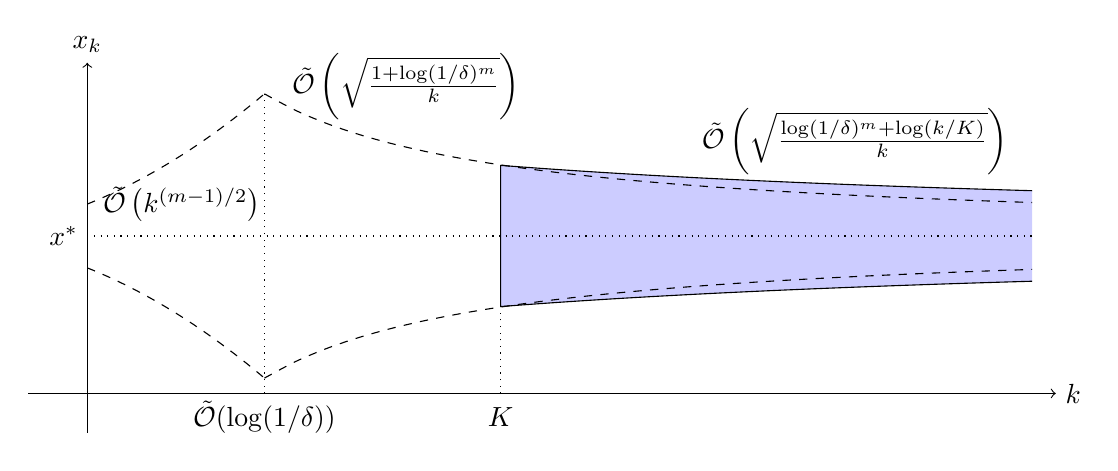
\begin{tikzpicture}[xscale=1.5]
  \draw[->] (-0.5, 0) -- (8.2, 0) node[right] {$k$};
  \draw[->] (0, -0.5) -- (0, 4.2) node[above] {$x_k$};

  \draw[fill=blue!20!white] plot[scale=0.5, domain=16:7, smooth, variable=\x, blue] ({\x},  {4+4.4*(1.9)^2/(\x+1)*ln(\x+1)/ln(10)}) -- plot[scale=0.5, domain=7:16, smooth, variable=\x, blue] ({\x}, {4-4.4*(1.9)^2/(\x+1)*ln(\x+1)/ln(10)});

  \draw[dashed,scale=0.5, domain=0:3, smooth, variable=\x] plot ({\x}, {4+(\x/3+0.9)^2});
  \draw[dashed,scale=0.5, domain=3:16, smooth, variable=\x] plot ({\x}, {4+4*(1.9)^2/(\x+1)});
  \draw[dashed,scale=0.5, domain=0:3, smooth, variable=\x] plot ({\x}, {4-(\x/3+0.9)^2});
  \draw[dashed,scale=0.5, domain=3:16, smooth, variable=\x] plot ({\x}, {4-4*(1.9)^2/(\x+1)});
  
  \draw (6.5,3.2) node {$\tilde{\mathcal{O}}\left(\sqrt{\frac{\log(1/\delta)^{m}+\log(k/K)}{k}}\right)$};
  
  \draw (2.7,3.9) node {$\tilde{\mathcal{O}}\left(\sqrt{\frac{1+\log(1/\delta)^{m}}{k}}\right)$};
  \draw (0.8,2.4) node {$\tilde{\mathcal{O}}\left(k^{(m-1)/2}\right)$};

  \draw[dotted] (0,2) -- (8,2);
  \draw (-0.2,2) node {$x^*$};

  \draw[dotted] (3.5,0) -- (3.5,2);
  \draw (3.5,-0.3) node {$K$};
  
  \draw[dotted] (1.5,0) -- (1.5,3.8);
  \draw (1.5,-0.3) node {$\tilde{\mathcal{O}}(\log(1/\delta))$};
\end{tikzpicture}
    \caption{For $D>0$, all the iterates lie in the blue shaded area with probability at least $1-\delta$.}
    \label{fig:anytimeBounded}
\end{figure}







Maximal concentration bounds immediately imply concentration bounds for a fixed iteration number (cf. Corollary \ref{cor:bounded}), which in turn gives the full tail bound (cf. Corollary \ref{cor:boundedTail}) and the sample complexity result (cf. Corollary \ref{co:sc}). For ease of exposition, we here only present the results when $D>0$. The case where $D=0$ can be derived in a straightforward manner.



\begin{corollary}[Fixed-Time Concentration] \label{cor:bounded}
Suppose that $D>0$. Under the same assumptions in Theorem \ref{thm:multi} (2), for any $\delta>0$ and $k\geq 0$, we have with probability at least $1-\delta$ that
\begin{align*}
	\|x_k-x^*\|_c^2
	\leq \;&\frac{c_1\alpha \|x_0-x^*\|_c^2}{k+h} \left[\log\left(\frac{m}{\delta}\right)+c_2+c_3+c_4\log\left(\frac{k-1+h}{h-1}\right)\right]^{m}.
\end{align*}
\end{corollary}

Corollary \ref{cor:bounded} follows by setting $K=k$ in Theorem \ref{thm:multi} (2).




\begin{corollary}[Full Tail Bound] \label{cor:boundedTail}
Suppose that $D>0$. Under the same assumptions in Theorem \ref{thm:multi} (2), there exists $C_1>0$ such that the following inequality holds for all $\epsilon>0$ and $k\geq 0$: 
\begin{align*}
    \mathbb{P}\left(\frac{\sqrt{k+h}\;\| x_k - x^* \|_c}{(\log(k))^{m/2}}> \epsilon \right) < m\exp\left(-C_1\epsilon^{2/m} \right).
\end{align*}
\end{corollary}

Corollary \ref{cor:boundedTail} is a direct implication of Corollary \ref{cor:bounded}, and provides an upper bound for the whole complementary cumulative distribution function (CDF) of the error $\|x_k-x^*\|_c$ for any iterate $k\geq 0$, which can be integrated to obtain bounds for any moment of the error at any point in time.

\begin{corollary}\label{co:sc}
Given $\epsilon>0$, to achieve $\|x_k-x^*\|_c\leq \epsilon$ with probability at least $1-\delta$, the sample complexity is $\tilde{\mathcal{O}}((1+\log^{m}(1/\delta))\epsilon^{-2})$.
\end{corollary}

As we see from Corollary \ref{co:sc}, the sample complexity dependency on $\epsilon$ is $\tilde{\mathcal{O}}(\epsilon^{-2})$, which is known to be optimal (up to  a logarithmic factor). In addition, we have super-polynomial tail as $\delta$ appears as $\log^m(1/\delta)$ in the bound. 

\paragraph{Removing the Logarithmic Factors} In view of Theorem \ref{thm:multi} (2), the bound involves a product of logarithmic terms (i.e., $\mathcal{O}([\log(k)]^{m-1})$). It is possible to remove them at a cost of slightly compromising the tail. The result is presented in the following, where $c_1''$ is a constant (explicit expressions in Appendix \ref{ap:last_bootstrapping}).

\begin{theoremp}{\ref*{thm:multi}$'$}[Proof in Appendix \ref{ap:last_bootstrapping}]\label{thm:improved}
Under the same conditions in Theorem \ref{thm:multi} (2), for any $\delta\in (0,1)$ and $K\geq 0$, with probability at least $1-\delta$, we have for all $k\geq K$ that
\begin{align*}
    \|x_k-x^*\|_c^2\leq \;&c_1''\alpha_k \|x_0-x^*\|_c^2\left[\left(\log\left(\frac{m+1}{\delta}\right)\right)^m+1\right]\\
	&\times \left[\log\left(\frac{m+1}{\delta}\right)+c_2\left(\frac{h}{K+h}\right)^{\alpha D_0/2-1}+c_3+c_4\log\left(\frac{k-1+h}{K-1+h}\right)\right].
\end{align*}
\end{theoremp}

Note that Theorem \ref{thm:improved} implies that there exists $C_1'>0$ such that
\begin{align*}
    \mathbb{P}(\sqrt{k+h}\;\| x_k - x^* \|_c> \epsilon ) < (m+1)\exp\left(-C_1'\epsilon^{2/(m+1)}\right),\quad \forall\;k\geq 0,\epsilon>0.
\end{align*}
Compared with Corollary \ref{cor:boundedTail} of Theorem \ref{thm:multi}, we see that the rate is improved by a logarithmic factor but the tail is heavier.


\subsection{An Impossibility Result on the Tail Decay Rate}\label{sec:hard_example}

Theorem \ref{thm:multi} shows that SA with multiplicative noise is able to achieve an $\tilde{\mathcal{O}}(1/k)$ rate of convergence with a super-polynomial tail. One may ask if sub-Gaussian (or sub-exponential) tail is achievable. In this section, we show that it is impossible to obtain a general sub-exponential tail bound whenever we only obtain a super-polynomial one. 

\paragraph{Example Setup} Let $a\in (0,1)$ and $N\geq 1$, and let $\{Y_k\}$ be an i.i.d. sequence of real-valued random variables such that 
$\mathbb{P}\left(Y_k=a+N\right)=1/(N+1)$ and $\mathbb{P}\left(Y_k=a-1\right)=N/(N+1)$.
Let $F:\mathbb{R}^2\mapsto \mathbb{R}$ be an operator defined as
\begin{align*}
    F(x,y)=yx,\quad \forall\;x,y\in\mathbb{R}.
\end{align*}
Consider the $1$-dimensional stochastic iterative algorithm
\begin{align}\label{algo:example}
    x_0>0,\quad x_{k+1} =\;& x_k + \alpha_k (F(x_k,Y_k)-x_k),
\end{align}
where $\alpha_k>0$ is the stepsize. 
It can be easily verified that (1) $\Bar{F}(x):=\mathbb{E}[F(x,Y_0)]$ is a contraction mapping with contraction factor $\gamma_c=a\in (0,1)$, (2) $\mathbb{E}[F(x_k,Y_k)\mid \mathcal{F}_k]=\Bar{F}(x_k)$ for all $k\geq 0$, and (3) $|F(x_k,Y_k)-\Bar{F}(x_k)|\leq N(|x_k|+1)$ for all $k\geq 0$. Note that $D=a+N-1$ in this example. Since all assumptions needed to apply Theorem \ref{thm:multi} (and also Theorem \ref{thm:improved}) are satisfied, we have the following result. 

\begin{proposition}\label{thm:example}
Consider $\{x_k\}$ generated by Algorithm (\ref{algo:example}). Suppose that $\alpha_k=\alpha/(k+h)$, where $\alpha>1/(1-a)$ and $h$ is large enough so that $\alpha_0<1/2$. Then, there exist $K_1,K_2,\Bar{K}_1,\Bar{K}_2>0$ such that the following inequalities hold for all $\epsilon>0$ and $k\geq 0$:
\begin{align}
    \mathbb{P}\left(\frac{\sqrt{k+h} \;x_k}{(\log(k))^{m_e/2}} > \epsilon \right) <\;&K_1 \exp\left(-K_2\epsilon^{\frac{2}{m_e}}\right),\label{eq:example_bound1}\\
    \mathbb{P}\left(\sqrt{k+h} \;x_k > \epsilon \right) <\;&\Bar{K}_1 \exp\left(-\Bar{K}_2\epsilon^{\frac{2}{m_e+1}}\right)\label{eq:example_bound2}.
\end{align}
where $m_e=\lceil 2\alpha D \rceil +1$.
\end{proposition}
\begin{remark}
    Since Algorithm (\ref{algo:example}) starts with a positive $x_0$, by ensuring $\alpha_0< 1/2$ we have $x_k>0$ for all $k\geq 0$. Moreover, it is easy to see that $x^*=0$ in this example.
\end{remark}

We next investigate the lower bound of Algorithm (\ref{algo:example}) through the following theorem.

\begin{theorem}[Proof in Appendix \ref{pf:le:example}]\label{le:example}
Consider $\{x_k\}$ generated by Algorithm (\ref{algo:example}). Suppose that $\alpha_k=\alpha/(k+h)^z$, where $z\in (0,1]$, $\alpha>0$, and $h$ is chosen such that $\alpha_0<1/2$.
\begin{enumerate}[(1)]
    \item When $z=1$, for any ${\tilde{\beta}}>2/(1+2\alpha D)$, we have
\begin{align*}
    \liminf\limits_{k\to\infty} \mathbb{E}\left[\exp\left(\lambda \left[(k+h)^{1/2} x_k\right]^{\tilde{\beta}}\right)\right] = \infty,\quad \forall\;\lambda>0.
\end{align*}
As a result, there do not exist $K_1',K_2'>0$ such that $\mathbb{P}\left((k+h)^{1/2}\;x_k\geq \epsilon\right)\leq K_1'\exp\left(-K_2'\epsilon^{\tilde{\beta}}\right) $ for any $\epsilon>0$ and $k\geq 0$.
\item When $z\in (0,1)$, for any ${\tilde{\beta}},{\tilde{\beta}}'>0$, we have
\begin{align*}
    \liminf\limits_{k\to\infty} \mathbb{E}\left[\exp\left(\lambda (k+h)^{{\tilde{\beta}}'} x_k^{\tilde{\beta}}\right)\right] = \infty,\quad \forall\;\lambda>0.
\end{align*}
As a result, there do not exist $\tilde{K}_1',\tilde{K}_2'>0$ such that $\mathbb{P}\left((k+h)^{{\tilde{\beta}}'/{\tilde{\beta}}}\;x_k\geq \epsilon\right)\leq \tilde{K}_1'\exp\left(-\tilde{K}_2'\epsilon^{\tilde{\beta}}\right) $ for any $\epsilon>0$ and $k\geq 0$.
\end{enumerate}
\end{theorem}






Since ${\tilde{\beta}} > 2/(1+2\alpha D)\geq 2/(1+\lceil 2\alpha D\rceil) = 2/m_e$, Theorem \ref{thm:example} (1) implies that our concentration bound is almost tight in the sense that it has either the best tail decay rate (at least when $2\alpha D$ is an integer, cf. Figure \ref{fig:upper_and_lower_bounds}) but with a slightly worse decay rate in $k$ (cf. Eq. (\ref{eq:example_bound1})), or it has the right decay rate in $k$ but with a slightly compromised tail decay rate (cf. Eq. (\ref{eq:example_bound2})). In particular, this means that we obtain a sub-exponential tail upper bound whenever such bound is achievable (that is, when $D\leq 1/2\alpha$).


Note that, as an aside, Theorem \ref{le:example} (2) implies that not even super-polynomial tail bounds are possible when $\alpha_k=\alpha/(k+h)^z$ (with $z\in (0,1)$), for any polynomial rate of convergence. 

\begin{figure}[H]
    \centering
    \begin{tikzpicture}[xscale=1.5]
  \draw[->] (0.9, 0) -- (8.5, 0) node[right] {$D$};
  \draw[->] (2, -0.5) -- (2, 4.6) node[above] {$\beta$};
  
  \draw[thick, dashed, color=red] plot[scale=1, domain=1.5:8.4, smooth, variable=\x] ({\x},  {4.5/(1.5+(\x-2))});
  \draw[thick] (1,3) -- (2,3);
  \draw[thick] (2,1.5) -- (3.5,1.5);
  \draw[thick] (3.5,1) -- (5,1);
  \draw[thick] (5,3/4) -- (6.5,3/4);
  \draw[thick] (6.5,3/5) -- (8,3/5);
  \draw[thick] (8,1/2) -- (8.4,1/2);

  \draw[dotted] (3.5,0) -- (3.5,1.5);
  \draw[dotted] (5,0) -- (5,1);
  \draw[dotted] (6.5,0) -- (6.5,3/4);
  \draw[dotted] (8,0) -- (8,3/5);
  
  \draw (3.5,-0.3) node {$\frac{1}{2\alpha}$};
  \draw (5,-0.3) node {$\frac{1}{\alpha}$};
  \draw (6.5,-0.3) node {$\frac{3}{2\alpha}$};
  \draw (8,-0.3) node {$\frac{2}{\alpha}$};
  
  \draw (1.85,3) node {$2$};
  \draw (1.85,1.5) node {$1$};
\end{tikzpicture}
    \caption{Best tail exponent in Proposition \ref{thm:example} (black) vs. upper bound on best possible tail exponent given by Theorem \ref{le:example} (1)}
    \label{fig:upper_and_lower_bounds}
\end{figure}


\subsection{Stochastic Approximation with Sub-Gaussian Additive Noise}\label{sec:additive}

In this section, we also consider $\{x_k\}$ generated by Algorithm (\ref{algo:sa}), but with additive sub-Gaussian noise. We begin by stating our assumption. 

\begin{assumption}\label{ass:sub-Gaussian}
There exist $\Bar{\sigma}>0$ and a (possibly) dimension-dependent constant $c_d>0$ such that 
the following two inequalities hold for any $\mathcal{F}_k$-measurable random vector $v$ and $k\geq 0$:
\begin{align}
    \mathbb{E}\left[\exp\left(\lambda \langle F(x_k,Y_k) \!-\! \mathbb{E}\left[F(x_k,Y_k) | \mathcal{F}_k \right], v \rangle \right) \middle| \mathcal{F}_k \right] \!\leq& \exp\left(\lambda^2\Bar{\sigma}^2 \|v\|_{c,*}^2/2\right)\label{eq:sub-Gaussian_1},\;\forall\;\lambda>0,\\
    \mathbb{E}\left[ \exp\left( \lambda \left\| F(x_k,Y_k) \!-\! \mathbb{E}\left[F(x_k,Y_k) | \mathcal{F}_k\right] \right\|_c^2 \right) \middle| \mathcal{F}_k \right] \!\leq&  \left(1\!-\! 2 \lambda \Bar{\sigma}^2\right)^{-c_d/2},\; \forall\;\lambda\in \left(0,1/2\Bar{\sigma}^2\right) \label{eq:sub-Gaussian_2},
\end{align}
where $\|\cdot\|_{c,*}$ is the dual norm of the contraction norm $\|\cdot\|_c$.
\end{assumption}

Assumption \ref{ass:sub-Gaussian} can be viewed as a generalization of the standard definition of a random vector being norm sub-Gaussian \citep{jin2019short} to the case where we use an arbitrary norm $\|\cdot\|_c$ instead of $\|\cdot\|_2$. In fact, when $\|\cdot\|_c=\|\cdot\|_2$ and $c_d=d$, Eqs. (\ref{eq:sub-Gaussian_1}) and (\ref{eq:sub-Gaussian_2}) are exactly the equivalent definitions of sub-Gaussian random vectors \citep{jin2019short,wainwright2019high}. Since we use an arbitrary norm, we allow for a (possibly) different dimension-dependent constant $c_d$. One special case where Assumptions \ref{as:contraction}, \ref{as:unbiased}, and \ref{ass:sub-Gaussian} are satisfied is when the noise $Y_k$ is purely additive, and is either a martingale-difference sequence or an i.i.d. mean zero sequence with sub-Gaussian tail.






We now state the main result of this section. Unlike SA with multiplicative noise, we allow for polynomially decaying stepsizes $\alpha_k=\alpha/(k+h)^z$, where $z\in (0,1]$ and $\alpha,h>0$ are appropriately chosen constants. The parameters $\{\Bar{c}_i\}_{1\leq i\leq 5}$ and $\bar{D}_1\in (0,1)$ used in stating the following theorem are also constants. The explicit requirement on $\alpha$ and $h$, and the expressions of $\{\Bar{c}_i\}_{1\leq i\leq 5}$ and $\bar{D}_1$ are presented in Appendix \ref{subsec:pf:thm:additive}.

\begin{theorem}[Proof in Appendix \ref{subsec:pf:thm:additive}]\label{thm:additive}
Consider $\{x_k\}$ generated by Algorithm (\ref{algo:sa}). Suppose that Assumptions \ref{as:contraction}, \ref{as:unbiased}, and \ref{ass:sub-Gaussian} are satisfied. Then we have the following results.
\begin{enumerate}[(1)]
\item When $z=1$ and $\alpha>2/\Bar{D}_1$, for any $\delta>0$ and $K\geq 0$, we have with probability at least $1-\delta$ that the following inequality holds for all $k\geq K$:
    \begin{align*}
        \|x_k-x^*\|_c^2\leq\;&\frac{\bar{c}_1\log(1/\delta)}{k+h}+\bar{c}_2\|x_0-x^*\|_c^2\left(\frac{h}{k+h}\right)^{\Bar{D}_1\alpha/2}+\frac{\bar{c}_3+\bar{c}_4\log((k+1)/K^{1/2})}{k+h}.
    \end{align*}
\item When $z\in (0,1)$, $\alpha>0$, and $h\geq (\frac{4z}{\Bar{D}_1\alpha})^{1/(1-z)}$, 
 for any $\delta>0$ and $K\geq 0$, we have with probability at least $1-\delta$ that the following inequality holds for all $k\geq K$:
    \begin{align*}
        \|x_k-x^*\|_c^2\leq\;&\frac{\Bar{c}_1\log(1/\delta)}{(k+h)^z}+\bar{c}_2\|x_0-x^*\|_c^2\exp\left(-\frac{\Bar{D}_1\alpha}{2(1-z)}((k+h)^{1-z}-h^{1-z})\right)\\
        &+\frac{\bar{c}_5+\bar{c}_4\log((k+1)/K^{1/2})}{(k+h)^z}.
    \end{align*}
\end{enumerate}
\end{theorem}

We will discuss the implications of Theorem  \ref{thm:additive} in terms of its dependence on $\delta$, $K$, and $k$. First of all, since the probability tolerance level $\delta$ appears as $\log(1/\delta)$ in the norm-square bound, the norm error $\|x_k-x^*\|_c$ has a sub-Gaussian tail. As for the dependence on $K$ and $k$, Theorem \ref{thm:additive} implies that, with probability at least $1-\delta$, all the iterates lie in a cone with a radius of order 
\begin{align*}
    \tilde{\Theta}\left(\sqrt{(\log(1/\delta)+\log(k/K^{1/2}))k^{-z}}\right)
\end{align*}
for all $k\geq K$\footnote{For $z=1$, using the same supermartingale argument as in the proof of Theorem~\ref{thm:multi}, the radius can be made to be of order $\tilde{\Theta}(\sqrt{(\log(1/\delta)+\log(k/K))/k})$, yielding a smaller initial radius of order $\Theta(\sqrt{\log(1/\delta)/K)})$.}.


As a side note, observe that when $z=1$, the conditions on the stepsizes in Theorem \ref{thm:additive} imply that $\alpha$ must be bounded away from zero ($\alpha>2/\Bar{D}_1$ to be precise), with this bound being independent from $h$. However, when $z<1$, then $\alpha$ only needs to be positive. This coincides with what was observed in the literature studying the mean-square error \citep{chen2020finite,bhandari2018finite}. 

As a byproduct of the proof of Theorem \ref{thm:additive}, we obtain a fixed-time concentration bound of order $\Theta(\sqrt{k^{-z}})$, matching the rate obtained for fixed-time mean-square error bounds in existing literature \citep{chen2020finite,srikant2019finite}. 

\begin{proposition}[Fixed-Time Concentration]\label{cor:gaussian}
Under the same assumptions in Theorem \ref{thm:additive}, we have the following results.
\begin{itemize}
    \item[(1)] When $\alpha_k=\alpha/(k+h)$ with $\alpha>2/\Bar{D}_1$, for any $\delta\in(0,1]$, we have
    \begin{align*}
        \mathbb{P}\left(\|x_k-x^*\|_c^2\leq  \frac{\Bar{c}_1\log(1/\delta)}{k+h}+ \frac{\Bar{c}_2\|x_0-x^*\|_c^2h^{\Bar{D}_1\alpha/2}}{(k+h)^{\Bar{D}_1\alpha/2}}+\frac{\Bar{c}_3+\Bar{c}_4}{k+h}\right)\geq 1-\delta.
    \end{align*}
    \item[(2)] When $\alpha_k=\alpha/(k+h)^z$ with $z\in (0,1)$, for any $\delta\in(0,1]$, we have
    \begin{align*}
        \mathbb{P}\left(\|x_k-x^*\|_c^2\leq \frac{\Bar{c}_1\log(1/\delta)}{(k+h)^z}+\Bar{c}_2\|x_0-x^*\|_c^2e^{\frac{\Bar{D}_1\alpha}{2(1-z)}((k+h)^{1-z}-h^{1-z})}+\frac{\Bar{c}_4+\Bar{c}_5}{(k+h)^z}\right)\geq 1-\delta.
    \end{align*}
\end{itemize}
\end{proposition}

The fixed-time concentration bound is equivalent to the full tail bound presented below.

\begin{corollary}[Full Tail Bound]\label{cor:tailGaussian}
Under the same assumptions in Theorem \ref{thm:additive}, we have the following results.\\
(1) When $\alpha_k=\alpha/(k+h)$ with $\alpha>2/\Bar{D}_1$, for any $k\geq 0$, we have for any $\epsilon>0$ that
    \begin{align*}
        \mathbb{P}\left(\|x_k-x^*\|_c >   \epsilon \right) \leq \exp\left(-\frac{k+h}{\Bar{c}_1}\left(\epsilon^2-\bar{c}_2\|x_0-x^*\|_c^2\left(\frac{h}{k+h}\right)^{\Bar{D}_1\alpha/2}-\frac{\bar{c}_3+\bar{c}_4}{k+h}\right)\right).
    \end{align*}
(2) When $\alpha_k=\alpha/(k+h)^z$ with $z\in (0,1)$ and $h\geq (\frac{4z}{\Bar{D}_1\alpha})^{\frac{1}{1-z}}$, for any $k\geq 0$, we have for any $\epsilon>0$ that
    \begin{align*}
        \mathbb{P}\left(\|x_k\!-\!x^*\|_c \!>\!  \epsilon \right)\!\leq\! \exp\left(\!-\frac{(k\!+\!h)^z}{\Bar{c}_1}\left(\epsilon^2\!\!-\!\Bar{c}_2\|x_0\!-\!x^*\|_c^2e^{-\frac{\Bar{D}_1\alpha}{2(1-z)}((k+h)^{1\!-\!z}-h^{1\!-\!z})}\!-\!\frac{\Bar{c}_4+\Bar{c}_5}{(k+h)^z}\!\right)\!\right).
    \end{align*}
\end{corollary}

The proof of Corollary \ref{cor:tailGaussian} follows by representing the probability tolerance level $\delta$ from Proposition \ref{cor:gaussian} as a function of the accuracy tolerance level $\epsilon$. Observe that Corollary \ref{cor:tailGaussian} provides a sub-Gaussian upper bound for the whole complementary CDF of the error $\|x_k-x^*\|_c$, for any $k\geq 0$. Therefore, we can use the formula $\mathbb{E}[\|x_k-x^*\|_c^r]=\int_0^\infty \mathbb{P}(\|x_k-x^*\|_c^r>x)dx$ (where $r$ is a positive integer) to integrate this bound to obtain bounds for any moment of the error at any point in time. 


\subsection{Linear Stochastic Approximation}\label{sec:linearSA}

One special case of SA is linear SA presented below:
\begin{align}\label{algo:linear_sa}
    x_{k+1}=x_k+\alpha_k(A(Y_k)x_k-b(Y_k)),
\end{align}
where $\{Y_k\}$ (taking values in $\mathcal{Y}$) is a sequence of i.i.d. random variables with distribution $\nu$, and $A:\mathcal{Y}\mapsto \mathbb{R}^{d\times  d}$ and $b:\mathcal{Y}\mapsto \mathbb{R}^d$ are deterministic functions. Linear SA has wide applications, such as solving least-square problems and TD-learning in RL \citep{bertsekas1996neuro}. In this section, we formally show that linear SA can be equivalently remodeled as a contractive SA in the form of Algorithm (\ref{algo:sa}) with multiplicative noise. As a result, Theorem \ref{thm:multi} is applicable for us to establish super-polynomial high probability bounds of linear SA.

To study Algorithm (\ref{algo:linear_sa}), we impose the following two assumptions.

\begin{assumption}\label{as:linear_sa_boundedness}
 $A_{\max}:=\sup_{y\in\mathcal{Y}}\|A(y)\|_2<\infty$ and $b_{\max}:=\sup_{y\in\mathcal{Y}}\|b(y)\|_2< \infty$.
\end{assumption}

Assumption \ref{as:linear_sa_boundedness} is widely used in studying the asymptotic convergence \citep{bertsekas1996neuro} or finite-sample mean-square bounds \citep{srikant2019finite} of linear SA.

\begin{assumption}\label{as:Hurwitz}
    The matrix $\Bar{A}=\mathbb{E}_{Y\sim \nu}[A(Y)]$ is Hurwitz, i.e., the eigenvalues of $\Bar{A}$ have strictly negative real parts.
\end{assumption}

Assumption \ref{as:Hurwitz} is usually imposed to ensure the stability of Algorithm (\ref{algo:linear_sa}) \citep{srikant2019finite}. In fact, consider the ODE associated with Algorithm (\ref{algo:linear_sa}):
\begin{align}\label{ode:linear_sa}
    \dot{x}(t)=\Bar{A}x(t)-\Bar{b},
\end{align}
where $\Bar{b}:=\mathbb{E}_{Y\sim \nu}[b(Y)]$ \citep{borkar2009stochastic}.
When $\Bar{A}$ is Hurwitz, the following Lyapunov equation 
\begin{align*}
    \Bar{A}^\top P+P\Bar{A}+I_d=0
\end{align*}
has a unique positive definition solution \citep{khalil2002nonlinear}, denoted by $\Bar{P}$. It follows that the unique equilibrium point $x^*=\Bar{A}^{-1}\Bar{b}$ of ODE (\ref{ode:linear_sa}) is exponentially stable \citep{haddad2011nonlinear}, which in turn guarantees the asymptotic convergence of Algorithm (\ref{algo:linear_sa}) via the ODE method \citep{borkar2009stochastic}.

We next reformulate Algorithm (\ref{algo:linear_sa}) in the form of Algorithm (\ref{algo:sa}). Let $F_\beta:\mathcal{Y}\times \mathbb{R}^d\mapsto\mathbb{R}^d$ be defined as
\begin{align*}
    F_\beta(x,y)=\beta A(y)x-\beta b(y)+x,\quad \forall\;x\in\mathbb{R}^d,y\in\mathcal{Y},
\end{align*}
where $\beta= \frac{1}{2} \lambda^{-1}_{\max}(\Bar{A}^\top \Bar{P}\Bar{A})$. In this work, $\lambda_{\max}(\cdot)$ (respectively, $\lambda_{\min}(\cdot)$) returns the largest (respectively, smallest) eigenvalue of a symmetric matrix. Then Algorithm (\ref{algo:linear_sa}) can be equivalently written as
\begin{align*}
    x_{k+1}=x_k+\frac{\alpha_k}{\beta}(F_\beta(x_k,Y_k)-x_k),
\end{align*}
which is in the same form of Algorithm (\ref{algo:sa}) because we can absorb $\beta$ into the stepsize. We next show that Assumptions \ref{as:contraction}, \ref{as:unbiased}, and \ref{as:multi} are satisfied in the context of linear SA. Let $\|\cdot\|_{\Bar{P}}$ be a norm defined as $\|x\|_{\Bar{P}}=(x^\top \Bar{P} x)^{1/2}$ for all $x\in\mathbb{R}^d$.

\begin{proposition}[Proof in Appendix \ref{pf:prop:linear_sa}]\label{prop:linear_sa}
    Suppose that Assumptions \ref{as:linear_sa_boundedness} and \ref{as:Hurwitz} are satisfied. Then the following results hold.
    \begin{enumerate}[(1)]
        \item There exists $\Bar{\gamma}\in (0,1)$ such that the operator $\Bar{F}_\beta(\cdot):=\mathbb{E}_{Y\sim \nu}[F_\beta(\cdot,Y)]$ is a $\Bar{\gamma}$ -- contraction mapping with respect to $\|\cdot\|_{\Bar{P}}$.
        \item It holds for all $k\geq 0$ that $\mathbb{E}[\Bar{F}_\beta(x_k,Y_k)\mid \mathcal{F}_k]=\Bar{F}_\beta(x_k)$, where $\mathcal{F}_k$ is the $\sigma$-algebra generated by $\{Y_0,Y_1,\cdots,Y_{k-1}\}$.
        \item There exists $\hat{\sigma}>0$ such that $\|F_\beta(x_k,Y_k)-\Bar{F}_\beta(x_k)\|_{\Bar{P}}\leq \hat{\sigma}(\|x\|_{\Bar{P}}+1)$ for all $k\geq 0$.
    \end{enumerate}
\end{proposition}

Proposition \ref{prop:linear_sa} enables us to apply Theorem \ref{thm:multi} to establish the finite-sample high probability bound of Algorithm (\ref{algo:linear_sa}). The result is presented in the following.



\begin{theorem}\label{thm:linear_sa}
Suppose that Assumptions \ref{as:linear_sa_boundedness} and \ref{as:Hurwitz} are satisfied, and $\alpha_k=\alpha\beta/(k+h)$ with appropriately chosen $\alpha$ and $h$. Then, the same bound in Theorem \ref{thm:multi} (and Theorem \ref{thm:improved}) holds here. In addition, there exists an integer $m_\ell>0$ such that for any $\epsilon>0$ and $\delta\in (0,1)$, to achieve $\|x_k-x^*\|_{\Bar{P}}\leq \epsilon$ with probability at least $1-\delta$, the sample complexity is $\tilde{\mathcal{O}}((1+\log^{m_\ell}(1/\delta))\epsilon^{-2})$.
\end{theorem}

Theorem \ref{thm:linear_sa} is qualitatively similar to Theorem \ref{thm:multi} in that we achieve $\tilde{\mathcal{O}}(\epsilon^{-2})$ sample complexity in terms of the accuracy level $\epsilon$ and the bound has super-polynomial tail.


\subsection{Proof Sketch of Theorem \ref{thm:multi}}\label{sec:proofsketch}

We  here only present the proof sketch for Theorem \ref{thm:multi}. The proof of Theorem \ref{thm:additive} follows from a qualitatively similar approach. Our high-level idea is a novel bootstrapping argument. The first step is to establish a time-varying worst case bound as an initialization, which is done in Proposition \ref{prop:worst_case_bound}, and the second step is to establish the iterative refinement of bounds presented in Section \ref{subsec:challenge}, which is the focus this section.

Suppose that there exists $\delta>0$ and a \textit{non-decreasing} sequence $\{T_k(\delta)\}_{k\geq 0}$ such that 
\begin{align*}
    \mathbb{P}(\|x_k-x^*\|_c^2\leq  T_k(\delta),\forall\;k\geq 0)\geq 1-\delta.
\end{align*}
Our goal is to show that for any $\delta'>0$, there exists a sequence $T_k(\delta,\delta')=\mathcal{O}(T_k(\delta)\alpha_k)$ such that 
\begin{align}\label{eq:bootstrapping_recipe}
    \mathbb{P}(\|x_k-x^*\|_c^2\leq  T_k(\delta,\delta'),\forall\;k\geq 0)\geq 1-\delta-\delta',
\end{align}
thereby establishing the bootstrapping blueprint.

\paragraph{Step 1: Bounding the log-MGF of the Generalized Moreau Envelope}

To establish Eq. (\ref{eq:bootstrapping_recipe}), we develop a Lyapunov argument with a modified version of the log-MGF as the Lyapunov function.
Denote $E_k(\delta)=\{\|x_t-x^*\|_c^2\leq  T_t(\delta),\forall\,t=0,1,\cdots,k\}$. Note that we have by definition that $\{E_k(\delta)\}$ is a sequence of decreasing events, i.e., $E_{k+1}(\delta)\subseteq E_k(\delta)$, and satisfies $\mathbb{P}(E_k(\delta))\geq 1-\delta$ for any $k\geq 0$. Let $\lambda_k=\theta \alpha_k^{-1} T_k(\delta)^{-1}$, where $\theta$ is a tunable constant and $\alpha_k$ is the stepsize. Using a time-varying $\lambda_k$ as opposed to constant $\lambda$ in the proof of classical concentration inequalities (such as Hoeffding inequality)
is crucially important in our approach. For any $k\geq 0$, let
\begin{align*}
	Z_k=\log\left(\mathbb{E}\left[\exp\left(\lambda_k\mathds{1}_{E_k(\delta)} M(x_k-x^*)\right)\right]\right)
\end{align*}
be a modified version of the log-MGF. Here $M(\cdot)$ is the generalized Moreau envelope introduced in \cite{chen2020finite} as a \textit{smooth approximation} of the norm-square function $\frac{1}{2}\|\cdot\|_c^2$. The explicit definition of $M(\cdot)$ and its properties are summarized in Lemma \ref{prop:Moreau}. We view $Z_k$ as our Lyapunov function, and the key step in establishing Eq. (\ref{eq:bootstrapping_recipe}) is to derive a bound for $Z_k$. 

Working with $\mathbb{E}[\exp\left(\lambda_k\mathds{1}_{E_k(\delta)} M(x_k-x^*)\right)]$ presents new challenges, as the exponential nature of the MGF prevents us from exploiting the linearity of the expectation, which was used extensively in deriving mean-square bounds \citep{srikant2019finite,chen2020finite}. Instead, after representing $Z_{k+1}$ using $Z_k$, we have the expectation of a product of random variables. To overcome this challenge, we use a conditioning argument along with the Cauchy-Schwarz inequality and, most importantly, the time-varying $(1-\delta)-$ confidence bound $T_k(\delta)$. Eventually, we obtain the following inequality:
\begin{align}
		Z_k\leq\;&  W_1\left(\frac{h}{k+h}\right)^{\alpha D_0/2-1}+W_2,\quad \forall\;k\geq 0,\label{sketch:overall}
\end{align}
where $W_1$ and $W_2$ are (problem-dependent) constants. 


\paragraph{Step 2: An Exponential Supermartingale and Ville's Maximal Inequality}
Let $\{\overline{M}_k\}$ be a sequence of random variables defined as
\begin{align*}
	\overline{M}_k=\exp\left(\lambda_k\mathds{1}_{E_k(\delta)} M(x_k-x^*)-W_3\sum_{i=0}^{k-1}\alpha_i\right),\quad \forall\;k\geq 0,
\end{align*}
where $W_3$ is a constant. We show that $\{\overline{M}_k\}$ is a supermartingale with respect to the filtration $\{\mathcal{F}_k\}_{k\geq 0}$, which enables us to use Ville's maximal inequality together with Eq. (\ref{sketch:overall}) to establish a maximal concentration inequality. Specifically, we have for any $K\geq 0$ that
\begin{align*}
	&\mathbb{P}\left(\sup_{k\geq K}\left\{\lambda_k\mathds{1}_{E_k(\delta)} M(x_k-x^*)-W_3\sum_{i=0}^{k-1}\alpha_i\right\}> \epsilon\right)\\
	= \;&\mathbb{P}\left(\sup_{k\geq K}\left\{\exp\left(\lambda_k\mathds{1}_{E_k(\delta)} M(x_k-x^*)-W_3\sum_{i=0}^{k-1}\alpha_i\right)\right\}> e^\epsilon\right)\\
	\leq \;&\exp\left(W_1\left(\frac{h}{K+h}\right)^{\alpha D_0/2-1}+W_2-W_3\sum_{i=0}^{K-1}\alpha_i-\epsilon\right),
\end{align*}
where the last line follows from Ville’s maximal inequality and Eq. (\ref{sketch:overall}). By using the fact that the generalized Moreau envelope $M(\cdot)$ is an approximation of the norm-square function $\frac{1}{2}\|\cdot\|_c^2$, setting $K=0$, and mostly importantly, dividing by $\lambda_k=\mathcal{O}(\alpha_k^{-1}T_k^{-1}(\delta))$, we have for any $\delta'\in (0,1)$ that
\begin{align*}
	\mathds{1}_{E_k(\delta)} \|x_k-x^*\|_c^2
	\leq W_4\alpha_kT_k(\delta)(\log(1/\delta')+1):=T_k(\delta,\delta'),\quad \forall\;k\geq 0
\end{align*}
with probability at least $1-\delta'$, where $W_4>0$ is a constant. After using union bound to remove the indicator function, the previous inequality reads
\begin{align}\label{sketch:improved}
    \mathbb{P}(\|x_k-x^*\|_c^2
	\leq T_k(\delta,\delta'),\;\forall\;k\geq 0)\leq 1-\delta-\delta',
\end{align}
which establishes Eq. (\ref{eq:bootstrapping_recipe}) we desire. Theorem \ref{thm:multi} then follows by using Proposition \ref{prop:worst_case_bound} as an initialization and repeatedly using Eq. (\ref{sketch:improved}) to improve the bound. 

Looking back, using a time-varying $\lambda_k=\mathcal{O}(\alpha_k^{-1}T_k^{-1}(\delta))$ is the key to make sure that the new bound $T_k(\delta,\delta')$ is improved by a factor of $\alpha_k=\mathcal{O}(1/k)$ compared to the old bound $T_k(\delta)$.




\section{Applications in Reinforcement Learning}\label{sec:RL}

Consider an infinite horizon discounted Markov decision process (MDP) defined by a finite state-space $\mathcal{S}$, a finite action-space $\mathcal{A}$, a set of transition probability matrices $\{P_a\in\mathbb{R}^{|\mathcal{S}|\times|\mathcal{S}|}\mid a\in\mathcal{A}\}$, a reward function $\mathcal{R}:\mathcal{S}\times\mathcal{A}\mapsto[0,1]$, and a discount factor $\gamma\in (0,1)$. Note that in RL, the transition probabilities and the reward function are unknown to the agent. Given a stationary policy $\pi:\mathcal{S}\mapsto\Delta^{|\mathcal{A}|}$, where $\Delta^{|\mathcal{A}|}$ stands for the $|\mathcal{A}|$ -- dimensional probability simplex, its value function $V^\pi:\mathcal{S}\mapsto\mathbb{R}$ and $Q$-function $Q^\pi:\mathcal{S}\times\mathcal{A}\mapsto\mathbb{R}$ are defined as 
\begin{align*}
    V^\pi(s)=\;&\mathbb{E}_\pi\left[\sum_{k=0}^\infty\gamma^k\mathcal{R}(S_k,A_k)\;\middle|\;S_0=s\right],\quad \forall\;s\in\mathcal{S},\\
    Q^\pi(s,a)=\;&\mathbb{E}_\pi\left[\sum_{k=0}^\infty\gamma^k\mathcal{R}(S_k,A_k)\;\middle|\; S_0=s,A_0=a\right],\quad \forall\;(s,a)\in\mathcal{S}\times \mathcal{A},
\end{align*}
where we use the notation $\mathbb{E}_\pi[\,\cdot\,]$ to mean that the actions are selected based on the policy $\pi$. The goal is to find an optimal policy $\pi^*$ so that its value function $V^*$, or equivalently its $Q$-function $Q^*$, is uniformly maximized.

Since many RL algorithms can be modeled as a contractive SA algorithm for solving some variant of the Bellman equation \citep{bertsekas1996neuro}, our SA results provide a unified framework for establishing the concentration bounds. We next use our SA results to establish high probability bounds of popular RL algorithms such as off-policy TD-learning with generalized importance sampling factors, on-policy TD-learning with linear function approximation, and $Q$-learning.
To the best of our knowledge, concentration bounds (with super-polynomial tails) for off-policy TD have never been established in the literature before due to the combination of potentially unboundedness of the iterates and the multiplicative noise. 




\subsection{Off-Policy TD-Learning with Generalized Importance Sampling Factors}

TD-learning is a common approach for solving the policy evaluation problem (i.e., estimating the value function of a policy $\pi$), which, after combined with policy gradient, forms the celebrated actor-critic framework \citep{konda2000actor} for finding an optimal policy, thereby solving the RL problem. In TD-learning, there are two policies that play important roles in the algorithm. One is the policy $\pi$ we want to evaluate, called the target policy, and the other is the policy $\pi_b$ used to collect samples, called the behavior policy. When $\pi=\pi_b$, the corresponding algorithm is called on-policy TD, otherwise it is called off-policy TD. Compared with on-policy TD, off-policy TD has many advantages both practically and theoretically; see \cite{levine2020offline} for more details. 

Due to the popularity of off-policy learning, there are many variants of off-policy TD-learning proposed in the literature, such as $Q^\pi(\lambda)$ \citep{harutyunyan2016q}, TB$(\lambda)$ \citep{precup2000eligibility}, Retrace$(\lambda)$ \citep{munos2016safe}, and $Q$-trace \citep{chen2021finite}, etc. A unified approach for establishing finite-sample mean-square bounds of these algorithms was presented in \cite{chen2021GB}. To establish the concentration bounds, we next present the generic framework of importance sampling based multi-step off-policy TD-learning presented in \cite{chen2021GB}.

Recall that we use $\pi$ as the target policy and $\pi_b$ as the behavior policy. Let $c,\rho:\mathcal{S}\times\mathcal{A}\mapsto\mathbb{R}_+$ be the generalized importance sampling factors. We impose the following assumption on the behavior policy.

\begin{assumption}\label{as:off-TD}
It holds that $\{a\in\mathcal{A}\mid \pi(a|s)>0\}\subseteq\{a\in\mathcal{A}\mid \pi_b(a|s)>0\}$ for all $s\in\mathcal{S}$. In addition, the Markov chain $\{S_k\}$ induced by $\pi_b$ has a unique stationary distribution $\kappa_{S,b}\in\Delta^{|\mathcal{S}|}$, which satisfies $\kappa_{S,b}(s)>0$ for all $s\in\mathcal{S}$.
\end{assumption}

The first part of Assumption \ref{as:off-TD} is usually called the coverage assumption in the literature, which states that the support of the behavior policy should cover the support of the target policy. 

Let $\{(S_k^0,A_k^0,S_k^1,A_k^1,\cdots,S_k^n,A_k^n)\}_{k\geq 0}$ be a sequence of i.i.d. samples such that $S_k^0\sim \kappa_{S,b}(\cdot)$, $A_k^i\sim \pi_b(\cdot|S_k^i)$, and $S_k^{i+1}\sim P_{A_k^i}(S_k^i,\cdot)$ for all $i\in \{0,1,\cdots,n\}$, where $n$ is a non-negative integer. In this paper, we assume i.i.d. sampling for RL algorithms, which is satisfied when there is a generative model. In practice, sometimes an RL algorithm is also implemented with a single trajectory of Markovian samples (generated by applying some suitable behavior policy to the underlying MDP). We want to point out that our current SA results do not allow for such Markovian sampling because we require the noise to be unbiased; see Assumption \ref{as:unbiased}. Studying SA with Markovian noise is an immediate future direction. That being said, existing concentration results studying SA with Markovian noise all require the iterates to be bounded by a deterministic constant \citep{qu2020finite,li2020sample}, and hence are not applicable to either off-policy TD-learning or on-policy TD-learning with linear function approximation.




We consider evaluating the $Q$-functions. The algorithm and results can easily be extended to TD-learning for evaluating the $V$-functions. The importance sampling based $n$-step off-policy TD-learning algorithm updates the estimate $Q_k$ of the target value function $Q^\pi$ according to
\begin{align}\label{algo:V-trace}
	Q_{k+1}(s,a)=\;&
	Q_k(s,a)+\alpha_k(s,a)\sum_{i=k}^{k+n-1}\gamma^{i-k}\prod_{j=k+1}^ic(S_k^j,A_k^j)\nonumber\\
	&\times \left(\mathcal{R}(S_k^i,A_k^i)+\gamma\rho(S_k^{i+1},A_k^{i+1})Q_k(S_k^{i+1},A_k^{i+1})-Q_k(S_k^i,A_k^i)\right)
\end{align}
when $(s,a)=(S_k^0,A_k^0)$, and $Q_{k+1}(s,a)=Q_k(s,a)$ otherwise. To understand Algorithm (\ref{algo:V-trace}), consider the special case of choosing the generalized importance sampling factors as $c(s,a)=\rho(s,a)=\pi(a|s)/\pi_b(a|s)$ for all $(s,a)$. Then Algorithm (\ref{algo:V-trace}) reduces to the classical on-policy $n$-step TD-learning \citep{sutton2018reinforcement} when $\pi=\pi_b$, and vanilla off-policy TD  when $\pi\neq \pi_b$. More generally, the factors $c(\cdot,\cdot)$ and $\rho(\cdot,\cdot)$ can be modified to trade off the bias and the variance in importance sampling based TD-learning algorithms. As a result of such trade-off, the limit of Algorithm (\ref{algo:V-trace}) is biased from the target value function $Q^\pi$, and is denoted by $Q_{\pi,\rho}$.
See \cite{chen2021GB} for more details.


We next remodel Algorithm (\ref{algo:V-trace}) in the form of Algorithm (\ref{algo:sa}), and verify that Assumptions \ref{as:contraction}, \ref{as:unbiased}, and \ref{as:multi} are satisfied. Let $\{Y_k\}_{k\geq 0}$ be an i.i.d. sequence defined as $Y_k=(S_k^0,A_k^0,S_k^1,A_k^1,\cdots,S_k^n,A_k^n)$ for all $k\geq 0$. Denote the distribution of $Y_k$ by $\kappa_{Y,b}$. Let $F:\mathbb{R}^{|\mathcal{S}|}\times\mathcal{Y}\mapsto\mathbb{R}^{|\mathcal{S}|}$ be an operator defined as
\begin{align*}
    &[F(Q,y)](s,a)
    =\;[F(Q,s_0,a_0,...,s_n,a_n)](s,a)\\
    =\;&\mathds{1}_{\{(s_0,a_0)=(s,a)\}}\sum_{i=0}^{n-1}\gamma^i\prod_{j=1}^ic(s_j,a_j)(\mathcal{R}(s_i,a_i)+\gamma \rho(s_{i+1},a_{i+1})Q(s_{i+1},a_{i+1})-Q(s_i,a_i))\\
    &+Q(s,a)
\end{align*}
for all $Q\in\mathbb{R}^{|\mathcal{S}||\mathcal{A}|}$ and $y\in\mathcal{Y}$. Then, Algorithm (\ref{algo:V-trace}) can be equivalently written as
\begin{align*}
	Q_{k+1}=Q_k+\alpha_k(F(Q_k,Y_k)-Q_k).
\end{align*}
The next proposition shows that Assumptions \ref{as:contraction}, \ref{as:unbiased}, and \ref{as:multi} are satisfied in the context of off-policy TD. The result was previous established in \cite{chen2021GB} for mean-square analysis, and was restated here for completeness.


\begin{proposition}\label{prop:offTD}
Suppose that Assumption \ref{as:off-TD} is satisfied, and the generalized importance sampling factors satisfy (1) $\rho(s,a)\geq c(s,a)$ for all $(s,a)$ and (2) $\max_{s}\sum_{a}\pi_b(a|s)\rho(s,a)\leq 1/\gamma$. Then we have the following results.
\begin{enumerate}[(1)]
	\item There exists $\gamma_o\in (0,1)$ such that the operator $\bar{F}(\cdot):=\mathbb{E}_{Y\sim \kappa_{Y,b}}[F(\cdot,Y)]$ is a $\gamma_o$ -- contraction mapping with respect to $\|\cdot\|_\infty$.
	\item It holds that $\mathbb{E}[F(Q_k,Y_k)\mid \mathcal{F}_k]=\bar{F}(Q_k)$ a.s. for all $k\geq 0$, where $\mathcal{F}_k$ is the $\sigma$-algebra generated by $\{Y_0,Y_2,\cdots,Y_{k-1}\}$.
	\item There exists $L_o>0$ such that $\|F(Q_k,Y_k)-\Bar{F}(Q_k)\|_\infty\leq L_o(1+\|Q_k\|_\infty)$
	for all $k\geq 0$.
\end{enumerate}
\end{proposition}




We next apply Theorem \ref{thm:multi} to establish the concentration bounds of off-policy TD-learning with generalized importance sampling factors. The parameter $n_{o}$ used to present the following theorem is a positive integer, and $\{c_{o,i}\}_{1\leq i\leq 5}$ and $D_o\in (0,1)$ are positive constants.






\begin{theorem}\label{thm:V-trace}
Consider $\{Q_k\}$ generated by Algorithm (\ref{algo:V-trace}). Suppose that Assumption \ref{as:off-TD} is satisfied, the generalized importance sampling factors $c(\cdot,\cdot)$ and $\rho(\cdot,\cdot)$ satisfy (1) $\rho(s,a)\geq c(s,a)$ for all $(s,a)$, and (2) $\max_{s}\sum_{a}\pi_b(a|s)\rho(s,a)\leq 1/\gamma$, and $\alpha_k=\alpha/(k+h)$ with $\alpha>2/D_o$ and $h$ large enough. Then, for any $\delta>0$ and $K\geq 0$, with probability at least $1-\delta$, we have for all $k\geq K$ that
    \begin{align*}
	\|Q_k-Q_{\pi,\rho}\|_\infty^2
	\leq \;&\frac{\alpha c_{o,1}\|Q_0-Q_{\pi,\rho}\|_c^2}{k+h}\left[ \left(\log\left(\frac{n_{o}+1}{\delta}\right)\right)^{n_{o}-1}+c_{o,2}\right]\nonumber\\
	&\times \bigg[\!\log\left(\frac{n_{o}\!+\!1}{\delta}\right)\!+\!c_{o,3}\left(\frac{h}{K+h}\right)^{\alpha D_o/2-1}\!\!\!+\!c_{o,4}\!+\!c_{o,5}\log\left(\frac{k-1+h}{K-1+h}\right)\bigg].
\end{align*}
\end{theorem}

Theorem \ref{thm:V-trace} implies that off-policy TD-learning enjoys an $\tilde{\mathcal{O}}(1/k)$ rate of convergence with super-polynomial tail, and appears to be the first result in the literature that establishes concentration bounds of off-policy TD-learning.


\subsection{On-Policy TD-Learning with Linear Function Approximation}

In this section, we consider on-policy TD-learning with linear function approximation, where function approximation is introduced to overcome the curse of dimensionality in RL. 


Given a target policy $\pi$, consider approximating $V^\pi$ from a linear sub-space of $\mathbb{R}^{|\mathcal{S}|}$ spanned by $d$ basis vectors $\phi_i\in\mathbb{R}^{|\mathcal{S}|}$, $1\leq i\leq d$. That is, we approximate $V^\pi$ using $V_\theta=\sum_{i=1}^d\phi_i\theta_i$, where $\theta\in\mathbb{R}^d$ is the weight vector. We assume without loss of generality that $\{\phi_i\}_{1\leq i\leq d}$ are linearly independent and are uniformly bounded such that $\max_{s\in\mathcal{S}}\|\phi(s)\|_2\leq 1$. We also denote $\Phi=[\phi_1,\phi_2\cdots,\phi_d]\in\mathbb{R}^{|\mathcal{S}|\times d}$ as the feature matrix and $\phi(s)=(\phi_1(s),\phi_2(s),\cdots,\phi_d(s))\in\mathbb{R}^d$ as the feature vector associated with state $s$.  In addition, we impose the following assumption on the target policy $\pi$. 


\begin{assumption}\label{as:policy_TDLFA}
    The Markov chain $\{S_k\}$ induced by $\pi$ admits a unique stationary distribution $\kappa_S\in\Delta^{|\mathcal{S}|}$, which satisfies $\kappa_S(s)>0$ for all $s$.
\end{assumption}

Assumption \ref{as:policy_TDLFA} essentially states that the target policy $\pi$ should enable the agent to sufficiently explore the state-space, which is, to some extend, a necessary requirement for learning its value function. Let $\{(S_k,A_k,S_k')\}_{k\geq 0}$ be a sequence of i.i.d. samples such that $S_k\sim \kappa_S(\cdot)$, $A_k\sim \pi(\cdot|S_k)$, and $S_k'\sim P_{A_k}(S_k,\cdot)$. Then, with a deterministic initialization $\theta_0\in\mathbb{R}^d$, TD-learning with linear function approximation iteratively updates the weight vector $\theta_k$ according to
\begin{align}\label{algo:TDLFA}
    \theta_{k+1}=\theta_k+\alpha_k\phi(S_k)(\mathcal{R}(S_k,A_k)+\gamma \phi(S_k')^\top \theta_k-\phi(S_k)^\top \theta_k),
\end{align}
where $\{\alpha_k\}$ is a positive sequence of stepsizes \citep{sutton2018reinforcement}. Algorithm (\ref{algo:TDLFA}) can be interpreted as an SA algorithm for solving a projected Bellman equation; see \cite{tsitsiklis1997analysis} for more details.

In view of Eq. (\ref{algo:TDLFA}), TD-learning with linear function approximation can be modeled as a linear SA algorithm in the form of Algorithm (\ref{algo:linear_sa}). Formally, 
let $Y_k=(S_k,A_k,S_k')\in \mathcal{Y}:=\mathcal{S}\times \mathcal{A}\times \mathcal{S}$ for all $k\geq 0$. It is clear that $\{Y_k\}$ is also an i.i.d. sequence. Denote the distribution of $Y_k$ by $\kappa_Y$, which satisfies $\kappa_Y(s,a,s')=\kappa_S(s)\pi(a|s)P_a(s,s')$ for all $(s,a,s')$. Let $A_o:\mathbb{R}^d\times \mathcal{Y}\mapsto \mathbb{R}^d$ and  $b_o:\mathbb{R}^d\times \mathcal{Y}\mapsto \mathbb{R}^d$ be defined as
\begin{align*}
    A_o(y)=\;&A_o(s,a,s')=\phi(s)(\gamma \phi(s') -\phi(s))^\top,\quad \forall\;y=(s,a,s')\in\mathcal{Y},\\
    b_o(y)=\;&b_o(s,a,s')=-\phi(s)\mathcal{R}(s,a),\quad \forall\;y=(s,a,s')\in\mathcal{Y}.
\end{align*}
Then Algorithm (\ref{algo:TDLFA}) can be equivalently written as 
\begin{align}\label{algo:TDLFA_reformulation}
    \theta_{k+1}=\;&\theta_k+\alpha_k(A_o(Y_k)\theta_k-b_o(Y_k)),\quad \forall\;k\geq 0.
\end{align}
We next verify that Assumptions \ref{as:linear_sa_boundedness} and \ref{as:Hurwitz} are satisfied in the context of TD-learning with linear function approximation. Let $\mathcal{K}_S=\text{diag}(\kappa_S)\in\mathbb{R}^{|\mathcal{S}|\times |\mathcal{S}|}$.


\begin{proposition}[Proof in Appendix \ref{pf:prop:TDLFA}]\label{prop:TDLFA}
Suppose that Assumption \ref{as:policy_TDLFA} is satisfied. Then the following results hold.
\begin{enumerate}[(1)]
    \item It holds for all $y\in\mathcal{Y}$ that $\|A_o(y)\|_2\leq 2$ and $\|b_o(y)\|_2\leq 1$.
    \item The matrix $\Bar{A}_o:=\mathbb{E}_{Y\sim \kappa_Y}[A_o(Y)]$ is Hurwitz.
\end{enumerate}
\end{proposition}


Proposition \ref{prop:TDLFA} enables us to apply Theorem \ref{thm:linear_sa} to establish the sample complexity bound of TD-learning with linear function approximation. Let $\theta^*$ be the unique solution to the equation $\Bar{A}_o\theta=\Bar{b}_o$, where $\Bar{b}_o=\mathbb{E}_{Y\sim \kappa_Y}[b_o(Y)]$.




\begin{theorem}\label{thm:TD}
Consider $\{\theta_k\}$ generated by Algorithm (\ref{algo:TDLFA}). Suppose that Assumption \ref{as:policy_TDLFA} is satisfied, and $\alpha_k=\alpha/(k+h)$ with appropriately chosen $\alpha$ and $h$. Then, there exists an integer $m_o>0$ such that for any $\epsilon>0$ and $\delta\in (0,1)$, to achieve $\|\theta_k-\theta^*\|_2\leq \epsilon$ with probability at least $1-\delta$, the sample complexity is $\tilde{\mathcal{O}}((1+\log^{m_o}(1/\delta))\epsilon^{-2})$.
\end{theorem}

\subsection{$Q$-Learning}\label{subsec:Q-learning}

So far we have been studying variants of TD-learning, which are usually used in an actor-critic framework to find an optimal policy. Another popular method for solving RL problems is the celebrated $Q$-learning algorithm \citep{watkins1992q}, which is the focus of this section. The $Q$-learning algorithm finds an optimal policy $\pi^*$ by finding the optimal $Q$-function $Q^*=Q^{\pi^*}$, the motivation of which is that $\pi^*(\cdot|s)$ is supported on the set $ {\arg\max}_{a\in\mathcal{A}}Q^*(s,a)$ for all $s\in\mathcal{S}$. See \cite{sutton2018reinforcement,bertsekas1996neuro} for more details about $Q$-learning.

Let $\pi_b$ be the behavior policy, which satisfies the following assumption.

\begin{assumption}\label{as:Q-learning}
    The Markov chain $\{S_k\}$ induced by $\pi_b$ admits a unique stationary distribution $\kappa_b\in\Delta^{|\mathcal{S}|}$, which satisfies $\kappa_b(s)>0$ for all $s$.
\end{assumption}

With a sequence of i.i.d. samples $\{(S_k,A_k,S_k')\}$ generated as $S_k\sim \kappa_b(\cdot)$, $A_k\sim \pi_b(\cdot|S_k)$, and $S_k'\sim P_{A_k}(S_k,\cdot)$ for all $k\geq 0$, the $Q$-learning algorithm iteratively updates an estimate $Q_k$ of $Q^*$ according to
\begin{align*}
    Q_{k+1}(s,a)=Q_k(s,a)+\alpha_k \mathds{1}_{\{(S_k,A_k)=(s,a)\}}(\mathcal{R}(S_k,A_k)+\gamma \max_{a'\in\mathcal{A}}Q_k(S_k',a')-Q_k(S_k,A_k))
\end{align*}
for all $(s,a)$ and $k\geq 0$, where $Q_0$ is initialized arbitrarily but satisfies $\|Q_0\|_\infty\leq 1/(1-\gamma)$. 

We next remodel $Q$-learning in the form of Algorithm (\ref{algo:sa}). Let $F:\mathbb{R}^{|\mathcal{S}||\mathcal{A}|}\times \mathcal{S}\times \mathcal{A}\times \mathcal{S}\mapsto \mathbb{R}^{|\mathcal{S}||\mathcal{A}|} $ be an operator defined as
\begin{align*}
    [F(Q,s_0,a_0,s_1)](s,a)=\mathds{1}_{\{(s_0,a_0)=(s,a)\}}(\mathcal{R}(s_0,a_0)+\gamma \max_{a'\in\mathcal{A}}Q(s_1,a')-Q(s_0,a_0))+Q(s,a)
\end{align*}
for all $(s,a)$ and $(Q,s_0,a_0,s_1)$. Then the update of $Q$-learning can be equivalently written as
\begin{align*}
    Q_{k+1}=Q_k+\alpha_k (F(Q_k,S_k,A_k,S_k')-Q_k),
\end{align*}
which is in the same form of SA algorithm (\ref{algo:sa}) with $x_k$ being $Q_k$ and $Y_k$ being the triple  $(S_k,A_k,S_k')$.
We next show that $Q$-learning is a contractive SA with sub-Gaussian additive noise. Before that, we need to introduce some notation. Let $\mathcal{H}:\mathbb{R}^{|\mathcal{S}||\mathcal{A}|}\mapsto\mathbb{R}^{|\mathcal{S}||\mathcal{A}|}$ be the Bellman optimality operator defined as
\begin{align*}
    [\mathcal{H}(Q)](s,a)=\mathcal{R}(s,a)+\gamma\mathbb{E}\left[\max_{a'\in\mathcal{A}}Q(S_1,a')\;\middle|\; S_0=s,A_0=a\right],\;\forall\;(s,a)\text{ and }Q\in \mathbb{R}^{|\mathcal{S}||\mathcal{A}|}.
\end{align*}
Let $D_b$ be an $|\mathcal{S}||\mathcal{A}|$ by $ |\mathcal{S}||\mathcal{A}|$ diagonal matrix with diagonal components $\{\kappa_b(s)\pi_b(a|s)\}$. Denote the minimum diagonal entry of  $D_b$ by $D_{b,\min}$. Let $\mathcal{F}_k$ be the $\sigma$-algebra generated by $\{S_i,A_i,S_i'\}_{0\leq i\leq k-1}$. Note that $Q_k$ is measurable with respect to $\mathcal{F}_k$. 

\begin{proposition}[Proof in Appendix \ref{pf:prop:Q-learning}]\label{prop:Q-learning}
    The operator $\bar{F}(\cdot):=\mathbb{E}[F(\cdot,S_k,A_k,S_k')]$ is explicitly given as
    \begin{align*}
        \bar{F}(Q)=D_b\mathcal{H}(Q)+(I_{|\mathcal{S}||\mathcal{A}|}-D_b)Q,\quad \forall\;Q\in\mathbb{R}^{|\mathcal{S}||\mathcal{A}|}.
    \end{align*}
    In addition, we have the following results.
    \begin{enumerate}[(1)]
        \item $\bar{F}(\cdot)$ is a $\hat{\gamma}_c$-contraction mapping with respect to $\|\cdot\|_\infty$, where $\hat{\gamma}_c=1-D_{b,\min}(1-\gamma)$;
        \item $\bar{F}(Q_k)=\mathbb{E}[F(Q_k,S_k,A_k,S_k')\mid \mathcal{F}_k]$ for all $k\geq 0$;
        \item Assumption \ref{ass:sub-Gaussian} holds with $\bar{\sigma}=4/(1-\gamma)$ and $c_d=1$.
    \end{enumerate}
\end{proposition}

Proposition \ref{prop:Q-learning} enables us to apply Theorem \ref{thm:additive} to get maximal concentration bound of $Q$-learning, which is presented below.

\begin{theorem}[Proof in Appendix \ref{pf:thm:Q-learning}]\label{thm:Q-learning}
Suppose that Assumption \ref{as:Q-learning} is satisfied, $\alpha_k=\alpha/(k+h)$ with $\alpha>2/(1-\hat{\gamma}_c)$ and appropriately chosen $h$. Then for any $K\geq 0$, we have with probability at least $1-\delta$ that the following inequality holds for all $k\geq K$:
\begin{align*}
    \|Q_k-Q^*\|_\infty^2\leq\;&c_q\left[\frac{\log(1/\delta)}{k+h}+\left(\frac{h}{k+h}\right)^{(1-\hat{\gamma}_c)\alpha/2}+\frac{1+\log((k+1)/K^{1/2})}{k+h}\right],
\end{align*}
    where $c_q=\frac{\log(|\mathcal{S}||\mathcal{A}|)}{D_{b,\min}^3(1-\gamma)^5}$.
\end{theorem}

Since $D_{b,\min}$ is the minimum entry of the stationary distribution of the Markov chain $\{(S_k,A_k)\}$ induced by the behavior policy $\pi_b$, we have $D_{b,\min}\leq 1/(|\mathcal{S}||\mathcal{A}|)$. In the ideal case where we have uniform sampling, i.e., $D_{b,\min}= 1/(|\mathcal{S}||\mathcal{A}|)$, Theorem \ref{thm:Q-learning} implies that the sample complexity to achieve $\|Q_k-Q^*\|_\infty\leq \epsilon$ is $\tilde{\mathcal{O}}(|\mathcal{S}|^3|\mathcal{A}|^3(1-\gamma)^{-5}\epsilon^{-2})$.


\section{Conclusion}\label{sec:conclusions}

In this paper we establish maximal concentration bounds for general contractive SA with additive and multiplicative noise. Specifically, we show that the sample paths remains in a cone (with decaying radius) with high probability. Moreover, we showcase how these general bounds can be applied to many RL algorithms, obtaining performance guarantees that were not available in previous literature. In order to overcome the challenge of having unbounded iterates with multiplicative noise, we develop a novel bootstrapping argument that enables us to iteratively improve a potentially loose bound to a tighter one. The key steps involves bounding a modified version of the log-MGF of the error, and carefully constructing supermartingales to obtain maximal bounds.

We recognize two avenues of future work. On the theoretical side, one avenue would be to extend our results to allow the operator to have Markovian noise with a large conditional bias, or to extend them to the more challenging two-time scale SA case. On the applications side, the other avenue would be to apply our results to other algorithms beyond RL.


\section*{Acknowledgements} We would like to thank Prof. R. Srikant from the University of Illinois at Urbana-Champaign for the insightful comments about using the telescoping technique to establish maximal concentration bounds.














\bibliographystyle{apalike}
\bibliography{references}

\newpage

\begin{center}
    {\Large\bfseries Appendices}
\end{center}

\appendix





\section{Proof of Theorem \ref{thm:multi}}\label{sec:proof}

In existing literature, a popular way of analyzing SA algorithms is the Lyapunov method \citep{srikant2019finite,chen2019finitesample,chen2020finite}, where the construction of a suitable Lyapunov function is at the heart of the analysis. Due to the potential non-smoothness of the norm-square function $\|x\|_c^2$, inspired by \cite{chen2020finite}, we will work with the generalized Moreau envelope defined as
\begin{align*}
	M(x) = \min_{u\in\mathbb{R}^d} \left\{ \frac{1}{2}\|u\|_c^2 + \frac{1}{2\mu} \|x-u\|_s^2 \right\}, 
\end{align*}
where $\|\cdot\|_s$ is a smoothing norm chosen such that $\frac{1}{2}\|\cdot\|_s^2$ is an $L$-smooth function with respect to $\| \cdot \|_s$, and $\mu>0$ is a tunable constant. Intuitively, the generalized Moreau envelope is constructed as a smooth approximation of the norm-square function $\|x\|_c^2$, which itself is in general not smooth (e.g., $\|\cdot\|_\infty^2$). This was formally established in \cite[Lemma 2.1]{chen2020finite}, and is presented in the following lemma for completeness. Let $\ell_{cs}$ and $u_{cs}$ be two positive constants such that $\ell_{cs}\|x\|_s\leq  \|x\|_c\leq u_{cs}\|x\|_s$ for all $x\in\mathbb{R}^d$, which is always possible due to the equivalence between norms in finite dimensional spaces. We assume without loss of generality that $\ell_{cs}\in (0,1]$ and $u_{cs}\in [1,+\infty)$.





\begin{lemma}[Lemma 2.1 of \cite{chen2020finite}]\label{prop:Moreau}
	The generalized Moreau envelope $M(\cdot)$ has the following properties.
	\begin{enumerate}[(1)]
		\item The function $M(\cdot)$ is convex and is $L/\mu$ -- smooth with respect to $\|\cdot\|_s$.
		\item There exists a norm, denoted by $\|\cdot\|_M$, such that $M(x)=\frac{1}{2}\|x\|_M^2$ for all $x\in\mathbb{R}^d$. 
		\item It holds that $(1+\mu \ell_{cs}^2)^{1/2}\|x\|_M\leq \|x\|_c\leq (1+\mu u_{cs}^2)^{1/2}\|x\|_M$ for all $x\in\mathbb{R}^d$.
	\end{enumerate}
\end{lemma}


For simplicity of notation, we will denote $\ell_{cM}=(1+\mu \ell_{cs}^2)^{1/2}$, $u_{cM}=(1+\mu u_{cs}^2)^{1/2}$, and $\tilde{\gamma}_c=\gamma_c u_{cM}/\ell_{cM}$. The tunable parameter $\mu>0$ is chosen such that $\tilde{\gamma}_c<1$, which is always possible since $\gamma_c\in (0,1)$ and $\lim_{\mu\rightarrow 0}u_{cM}/\ell_{cM}=1$.







\subsection{Bounding the MGF of the Generalized Moreau Envelope}\label{subsec:step1}

For classical concentration inequalities such as Hoeffding's inequality and Chernoff bounds, the main proof idea is to first bound the MGF and then use Markov inequality. Inspired by this, we bound the MGF of some modified version of the generalized Moreau envelope. Similar ideas were also used in the development of the transform method for studying queueing systems \citep{hurtado2020transform}.

To prepare for the bootstrapping argument we develop to handle the challenge of having potentially unbounded iterates, we will construct a modified MGF in the following. Given $\delta\in (0,1)$, let $\{T_k(\delta)\}_{k\geq 0}$ be a positive \textit{non-decreasing} sequence such that 
\begin{align*}
    \mathbb{P}(\|x_k-x^*\|_c^2\leq  T_k(\delta),\forall\;k\geq 0)\geq 1-\delta.
\end{align*} 
Since $x_0$ is initialized deterministically, we must have $T_0(\delta)\geq \|x_0-x^*\|_c^2$ a.s. A trivial example of $\{T_k(\delta)\}$ here is to choose $T_k(\delta)=B_k^2(D)$, where $B_k(D)$ is the worst case almost sure bound provided in Proposition \ref{prop:worst_case_bound}. Denote $E_k(\delta)=\{\|x_t-x^*\|_c^2\leq  T_t(\delta),\forall\;t=0,1,\cdots,k\}$. Note that we have by definition that $\{E_k(\delta)\}_{k\geq 0}$ is a sequence of decreasing events, i.e., $E_{k+1}(\delta)\subseteq E_k(\delta)$, and satisfies $\mathbb{P}(E_k(\delta))\geq 1-\delta$ for any $k\geq 0$. Let $\lambda_k=\frac{\theta}{\alpha_k T_k(\delta)}$, where $\theta$ is a tunable constant yet to be chosen and $\alpha_k$ is the stepsize. For any $k\geq 0$, let
\begin{align*}
	Z_k=\log\left(\mathbb{E}\left[\exp\left(\lambda_k\mathds{1}_{E_k(\delta)} M(x_k-x^*)\right)\right]\right),
\end{align*}
which is the modified version of the log-MGF that will be frequently used in our analysis. To understand the intuition behind the definition of $Z_k$, suppose that $\|x_k-x^*\|_c$ is uniformly bounded by a deterministic constant, i.e., the case $D<0$ in Proposition \ref{prop:worst_case_bound}. Then we can choose $T_k(\delta)$ to be the constant worst case bound provided in Proposition \ref{prop:worst_case_bound} (3), which implies $\mathds{1}_{E_k(\delta)}=1$ a.s. In this case, $Z_k$ becomes the standard log-MGF. Since we do not have such strong boundedness property, we introduce the additional parameters $T_k(\delta)$ and $\mathds{1}_{E_k(\delta)}$. This is crucial for the development of our bootstrapping argument that is used to overcome the challenge of having unboundeness iterates. 

The first step in our proof is to establish a recursive bound of the sequence $\{Z_k\}$. Let $D_0=2(1-\tilde{\gamma}_c)\in (0,1)$, $D_1=\frac{4\sigma^2}{\ell_{cM}^2}$, and $D_2=\frac{2L(2+\sigma)^2u_{cM}^2}{\mu\ell_{cs}^2}$. We choose the parameter $\theta$ as
\begin{align*}
    \theta=\frac{D_0\|x_0-x^*\|_c^2}{8D_1((1+\|x^*\|_c)^2+\|x_0-x^*\|_c^2)}.
\end{align*}
Recall that we use $\alpha_k=\alpha/(k+h)$ as our stepsize, where $\alpha$ and $h$ are chosen such that the following condition is satisfied.

\begin{condition}
The parameter $\alpha$ satisfy $\alpha>2/D_0$ and $h>1$ is chosen such that $\alpha_0\leq \min(1,D_0,\frac{D_0}{4D_2})$.
\end{condition}

\begin{proposition}[Proof in Appendix \ref{pf:prop:MGF_recursive}]\label{prop:MGF_recursive}
	It holds for all $k\geq 0$ that
	\begin{align}
		&\mathbb{E}\left[\exp\left(\lambda_{k+1}\mathds{1}_{E_{k+1}(\delta)}M(x_{k+1}-x^*)\right)\mid\mathcal{F}_k\right]\nonumber\\
		\leq  \;&\exp\left(\exp\left(-\frac{\alpha D_0/2-1}{\alpha}\alpha_k\right)\lambda_k\mathds{1}_{E_k(\delta)}M(x_k-x^*)\right)\exp\left( 2\alpha_k^2 \lambda_k D_2(1+\|x^*\|_c)^2\right).\label{eq10:MGF_recursive}
	\end{align}
\end{proposition}

In view of Eq. (\ref{eq10:MGF_recursive}), a recursive bound of $\{Z_k\}$ can be obtained by first taking total expectation, then taking logarithm, and finally using Jensen's inequality. The result is presented in the following.

\begin{lemma}\label{le:MGFrecursive}
	It holds for all $k\geq 0$ that
	\begin{align*}
		Z_{k+1}\leq \exp\left(-\frac{\alpha D_0/2-1}{\alpha}\alpha_k\right)Z_k+2\alpha_k^2 \lambda_k D_2(1+\|x^*\|_c)^2.
	\end{align*}
\end{lemma}


Lemma \ref{le:MGFrecursive} provides us a recursive inequality between $Z_{k+1}$ and $Z_k$. Solving this recursion and we obtain the following overall bound on the modified log-MGF $Z_k$.

\begin{lemma}[Proof in Appendix \ref{pf:le:multi_solving_recursion}]\label{le:multi_solving_recursion}
	It holds for all $k\geq 0$ that
	\begin{align*}
		Z_k\leq  Z_0\left(\frac{h}{k+h}\right)^{\alpha D_0/2-1}+\frac{4\alpha e D_2}{\alpha D_0/2-1}\frac{(1+\|x^*\|_c)^2}{\|x_0-x^*\|_c^2}.
	\end{align*}
\end{lemma}

To this end, we have successfully established a recursive bound (cf. Proposition \ref{prop:MGF_recursive}) and an overall bound (cf. Lemma \ref{le:multi_solving_recursion}) of our modified log-MGF $Z_k$. The next step is to construct a supermartingale using $\{Z_k\}$ and apply Ville's maximal inequality to derive maximal concentration bounds.




\subsection{An Exponential Supermartingale and the First Maximal Bound}

Let $\{\overline{M}_k\}$ be a sequence of random variables defined as
\begin{align*}
	\overline{M}_k=\exp\left(\lambda_k\mathds{1}_{E_k(\delta)} M(x_k-x^*)-D_3\sum_{i=0}^{k-1}\alpha_i\right),\quad \forall\;k\geq 0,
\end{align*}
where $D_3= \frac{D_0D_2}{4D_1} $. The next lemma shows that $\{\overline{M}_k\}$ is a supermartingale with respect to the filtration $\{\mathcal{F}_k\}_{k\geq 0}$. 

\begin{lemma}[Proof in Appendix \ref{pf:le:supermartingale}]\label{le:super-martingale}
	The random process $\{\overline{M}_k\}$ is a supermartingale.
\end{lemma}

Now we have shown that $\{\overline{M}_k\}$ is a supermartingale, and provided a bound on the expectation of $\overline{M}_k$ (cf. Lemma \ref{le:multi_solving_recursion}). We next use Ville's maximal inequality to establish the first maximal concentration bound in Proposition \ref{prop:ville}.

\begin{proposition}[Proof in Appendix \ref{pf:prop:ville}]\label{prop:ville}
	For any $\delta'\in (0,1)$ and $K\geq 0$, with probability at least $1-\delta'$, we have 
	\begin{align}
		&\sup_{k\geq K}\left\{\lambda_k\mathds{1}_{E_k(\delta)} \|x_k-x^*\|_c^2\right\}\nonumber\\
	\leq \;&2u_{cM}^2\log(1/\delta')+\frac{2u_{cM}^2D_0}{16\alpha_0D_1\ell_{cM}^2}\left(\frac{h}{K+h}\right)^{\alpha D_0/2-1}+\frac{16u_{cM}^2\alpha e D_2}{\alpha D_0-2}\frac{(1+\|x^*\|_c)^2}{\|x_0-x^*\|_c^2}\nonumber\\
	&+2\alpha D_3 u_{cM}^2\log\left(\frac{k-1+h}{K-1+h}\right).\label{eq:first_concentration}
	\end{align}
\end{proposition}

Suppose that the iterates $\{x_k\}$ are uniformly bounded by a deterministic constant. Then by choosing $T_k(\delta)$ as the uniform norm-square bound and we have $\lambda_k=c/\alpha_k$ for some constant $c$ and $\mathds{1}_{\{E_k(\delta)\}}=1$ a.s. In this case, multiplying $\alpha_k$ on both sides of Eq. (\ref{eq:first_concentration}) and we obtain the desired concentration bound, which has $\tilde{\mathcal{O}}(1/k)$ rate and exponential tail $\mathcal{O}(\log(1/\delta'))$. However, in the case of multiplicative noise the iterates $\{x_k\}$ in general do not admit a uniform bound. Since $\lambda_k=\theta \alpha_k^{-1} T_k(\delta)^{-1}$ and $T_k(\delta)$ can be an increasing function, Eq. (\ref{eq:first_concentration}) does not provide us the right rate. Therefore, based on Proposition \ref{prop:ville}, we next develop a bootstrapping argument to iteratively improve the rate. 

\subsection{A Bootstrapping Argument}

Recall that we start with
\begin{align}\label{eq:22}
	\mathbb{P}(\|x_k-x^*\|_c^2\leq T_k(\delta),\forall\;k\geq 0)\geq 1-\delta,
\end{align} 
and arrive at Proposition \ref{prop:ville}. When choosing $K=0$ in Proposition \ref{prop:ville}, Eq. (\ref{eq:first_concentration}) is also a maximal concentration inequality. More formally, we have the following result.

\begin{proposition}[Proof in Appendix \ref{pf:prop:bootstrapping}]\label{prop:bootstrapping}
	For any $\delta, \delta'\in (0,1)$ and $K\geq 0$, with probability at least $1-\delta-\delta'$, we have for all $k\geq K$ that
	\begin{align*}
	\|x_k-x^*\|_c^2
	\leq \;&\frac{\alpha_k T_k(\delta)}{\theta} \bigg[2u_{cM}^2\log(1/\delta')+\frac{2u_{cM}^2D_0}{16\alpha_0D_1\ell_{cM}^2}\left(\frac{h}{K+h}\right)^{\alpha D_0/2-1}\nonumber\\
	&+\frac{16u_{cM}^2\alpha e D_2}{\alpha D_0-2}\frac{(1+\|x^*\|_c)^2}{\|x_0-x^*\|_c^2}+2\alpha D_3 u_{cM}^2\log\left(\frac{k-1+h}{K-1+h}\right)\bigg].
\end{align*}
\end{proposition}

After choosing $K=0$ in Proposition \ref{prop:bootstrapping}, the result reads: 
\begin{align*}
	\mathbb{P}(\|x_k-x^*\|_c^2\leq\;& T_k(\delta),\forall\;k\geq 0)\geq 1-\delta\\
	\Longrightarrow\;\mathbb{P}(\|x_i-x^*\|_c^2\leq\;& T_k(\delta,\delta'),\forall\;k\geq 0)\geq 1-\delta-\delta',
\end{align*}
where
\begin{align*}
	T_k(\delta,\delta')=\;&\frac{\alpha_k T_k(\delta)}{\theta} \bigg[2u_{cM}^2\log(1/\delta')+\frac{2u_{cM}^2D_0}{16\alpha_0D_1\ell_{cM}^2}\\
	&+\frac{16u_{cM}^2\alpha e D_2}{\alpha D_0-2}\frac{(1+\|x^*\|_c)^2}{\|x_0-x^*\|_c^2}+2\alpha D_3 u_{cM}^2\log\left(\frac{k-1+h}{h-1}\right)\bigg].
\end{align*}

In terms of the dependence on $k$, because of the multiplication of $\alpha_k$, the new bound $T_k(\delta,\delta)$ is roughly smaller by a factor of $1/k$ compared with the old bound $T_k(\delta)$. The previous inequality suggests the following bootstrapping argument to iteratively improve the result in Proposition \ref{prop:ville}. We start with the worst case a.s. bound derived in Proposition \ref{prop:worst_case_bound}, where in the case of $D\geq 0$ the bound $T_k(\delta)=B_k(D)^2$ grows either logarithmically or polynomially with respect to $k$. Then, we iteratively use Proposition \ref{prop:bootstrapping} to improve the bound. Since every time we apply Proposition \ref{prop:bootstrapping} the bound gets improved by a factor of roughly $1/k$, at some point, we will arrive at a bound $T_k(\delta,\delta_1,\delta_2,\cdots,\delta_m)$ (where $m$ stands for the number of times we bootstrap using Proposition \ref{prop:bootstrapping}) that is of the order $1/k$, in which case we obtain the desired rate and Proposition \ref{prop:bootstrapping} is no longer applicable because we require $T_k(\delta,\delta_1,\delta_2,\cdots,\delta_m)$ to be non-decreasing to initialize the bootstrapping argument. See the beginning of Appendix \ref{subsec:step1}.


We next formalize the above bootstrapping argument. In the case of $D>0$, we have assumed that $2\alpha D$ is a positive integer. In view of Proposition \ref{prop:worst_case_bound}, $\|x_k-x^*\|_c^2$ can be polynomially increasing at a rate of $\mathcal{O}(k^{2\alpha D})$. Therefore, we need to bootstrap $m:=2\alpha D+1$ times. When $D=0$, since $\|x_k-x^*\|_c^2$ can only grow logarithmically, we need to  only bootstrap once. Let
\begin{align*}
    D_4=\;&\frac{(1+\|x^*\|_c)^2}{\|x_0-x^*\|_c^2},\;c_1=\frac{32^mD_1^m(1+D_4)^mu_{cM}^{2m}}{D_0^m}\left(1+\frac{\sigma^2 D_4}{D^2}\right),\;c_2=\frac{D_0}{16\alpha_0D_1\ell_{cM}^2},\\
    c_3=\;&\frac{8\alpha e D_2D_4}{\alpha D_0-2},\;c_4=\alpha D_3,\;\text{ and }
    c_1'=\frac{32u_{cM}^2D_1 (1+\sigma D_4\alpha^2 )(D_4+1)}{D_0}.
\end{align*}


\begin{proposition}[Proof in Appendix \ref{pf:le:first_bootstrap}]\label{le:first_bootstrap}
	The following results hold.
	\begin{enumerate}[(1)]
	\item 
	When $D>0$, let $\delta>0$ be arbitrary. For any $K\geq 0$, with probability at least $1-\delta$, we have for all $k\geq K$ that
	\begin{align}\label{eq:before_last_bootstrapping}
	\|x_k\!-\!x^*\|_c^2
	\leq \;&c_1\alpha_k \|x_0\!-\!x^*\|_c^2 \left[\log\left(\frac{m}{\delta}\right)+c_2+c_3+c_4\log\left(\frac{k-1+h}{h-1}\right)\right]^{m-1}\nonumber\\
	&\times \left[\log\left(\frac{m}{\delta}\right)+c_2\left(\frac{h}{K+h}\right)^{\alpha D_0/2-1}\!\!+c_3+c_4\log\left(\frac{k-1+h}{K-1+h}\right)\right].
\end{align}
\item When $D=0$, for any $\delta>0$ and $K\geq 0$, with probability at least $1-\delta$, we have for all $k\geq K$ that
		\begin{align*}
	\|x_k-x^*\|_c^2
	\leq \;&c_1'\|x_0-x^*\|_c^2\alpha_k\left[\log\left(\frac{k-1+h}{h-1}\right)\right]^2\\
	&\times \left[\log\left(\frac{1}{\delta}\right)+c_2\left(\frac{h}{K+h}\right)^{\alpha D_0/2-1}+c_3+c_4 \log\left(\frac{k-1+h}{K-1+h}\right)\right].
\end{align*}
\end{enumerate}
\end{proposition}

The proof of Theorem  \ref{thm:multi} is now complete.

\subsection{Removing the Product of the Logarithmic Factors}\label{ap:last_bootstrapping}

In Proposition \ref{le:first_bootstrap} (1), while the polynomial term, i.e., $\alpha_k$, gives us the $\mathcal{O}(1/k)$ rate, there is a product of logarithmic terms (i.e., $\mathcal{O}([\log(k)]^{m-1})$). To remove them, we perform one more step of bootstrapping. Recall from Appendix \ref{subsec:step1} that we require the initial bound to be non-decreasing to initialize the bootstrapping argument. However, the RHS of Eq. (\ref{eq:before_last_bootstrapping}) will eventually be decreasing as the polynomial term $\alpha_k$ will dominate the logarithmic terms when $k$ is large enough. To overcome this difficulty, define
\begin{align*}
    \tilde{T}_k(\delta)=c_1\|x_0-x^*\|_c^2\sup_{0\leq k'\leq k}\left\{\alpha_{k'} \left[\log\left(\frac{m}{\delta}\right)+c_2+c_3+c_4\log\left(\frac{k'-1+h}{h-1}\right)\right]^m\right\}.
\end{align*}
for any $\delta>0$ and $k\geq 0$. Note that $T_k(\delta)$ is (by definition) a non-decreasing sequence, and Proposition \ref{le:first_bootstrap} (1) implies
\begin{align}\label{eq:need_for_last_bootstrap}
    \mathbb{P}\left(\|x_k-x^*\|_c^2\leq  \tilde{T}_k(\delta),\;\forall\;k\geq 0\right)\geq 1-\delta.
\end{align}
we are now ready to perform the additional bootstrapping step to remove the product of the logarithmic terms. The result is presented in the following. 

\begin{proposition}[Proof in Appendix \ref{pf:prop:last_bootstrapping}]\label{prop:last_bootstrapping}
	When $D>0$, for any $\delta\in (0,1)$ and $K\geq 0$, with probability at least $1-\delta$, we have for all $k\geq K$ that
\begin{align*}
    \|x_k-x^*\|_c^2\leq \;&c_1''\alpha_k \|x_0-x^*\|_c^2\left[\left(\log\left(\frac{m+1}{\delta}\right)\right)^m+1\right]\\
	&\times \left[\log\left(\frac{m+1}{\delta}\right)+c_2\left(\frac{h}{K+h}\right)^{\alpha D_0/2-1}+c_3+c_4\log\left(\frac{k-1+h}{K-1+h}\right)\right],
\end{align*}
where 
\begin{align*}
    c_1''=\;&\frac{(64 D_1(1+D_4)u_{cM}^2)^{m+1}}{D_0^{m+1}}\left(1+\frac{\sigma^2 D_4}{D^2}\right)\\
    &\times \left(1+\sup_{k'\geq 0}\left\{\alpha_{k'} \left(c_2+c_3+c_4\log\left(\frac{k'-1+h}{h-1}\right)\right)^m\right\}\right).
\end{align*}
\end{proposition}

\subsection{Proof of All Technical Results in Support of Theorem \ref{thm:multi}}

\subsubsection{Proof of Proposition \ref{prop:worst_case_bound}}\label{pf:prop:worst_case_bound}
Using the update equation (\ref{algo:sa}) and the fact that $\Bar{F}(x^*)=x^*$, we have for all $k\geq 0$ that
\begin{align*}
	x_{k+1}-x^*=x_k-x^*+\alpha_k(F(x_k,Y_k)-\Bar{F}(x_k)+\Bar{F}(x_k)-\Bar{F}(x^*)+x^*-x_k).
\end{align*}
It follows that
\begin{align*}
	\|x_{k+1}-x^*\|_c\leq\;& (1-\alpha_k)\|x_k-x^*\|_c+\alpha_k(\|F(x_k,Y_k)-\Bar{F}(x_k)\|_c+\|\Bar{F}(x_k)-\Bar{F}(x^*)\|_c)\\
	\leq\;& (1-\alpha_k)\|x_k-x^*\|_c+\alpha_k(\sigma(1+\|x_k\|_c)+\gamma_c\|x_k-x^*\|_c)\\
	\leq\;& (1-\alpha_k)\|x_k-x^*\|_c+\alpha_k(\sigma\|x_k-x^*\|_c+\sigma(1+\|x^*\|_c)+\gamma_c\|x_k-x^*\|_c)\\
	=\;& (1+(\sigma+\gamma_c-1)\alpha_k)\|x_k-x^*\|_c+\alpha_k\sigma(1+\|x^*\|_c)\\
	=\;& (1+D\alpha_k)\|x_k-x^*\|_c+\alpha_k\sigma(1+\|x^*\|_c)
\end{align*}
where the second inequality follows from Assumption \ref{as:contraction} and Assumption \ref{as:multi}. To proceed, we need the following lemma, which is a general result on solving recursive inequalities.



\begin{lemma}\label{le:help1}
	Consider a scalar-valued sequence $\{w_k\}$ defined as
	\begin{align*}
		w_{k+1}=(1+\beta_1\alpha_k)w_k+\beta_2 \alpha_k,\quad \forall\;k\geq 0,
	\end{align*}
	where $w_0\geq 0$, $\{\alpha_k\}$ is a sequence of positive real numbers, and $\beta_1\in (-1/\alpha_0,\infty)$, $\beta_2>0$ are constants. Then, we have for all $k\geq 0$ that
	\begin{align*}
		w_k\leq \begin{dcases}
			e^{\beta_1\sum_{i=0}^{k-1}\alpha_i}w_0+\frac{\beta_2}{\beta_1}(e^{\beta_1\sum_{i=0}^{k-1}\alpha_i}-1),& \beta_1>0,\\
			w_0+\beta_2\sum_{i=0}^{k-1}\alpha_i,&\beta_1=0,\\
			w_0-\frac{\beta_2}{\beta_1},&\beta_1<0.
		\end{dcases}
	\end{align*}
\end{lemma}
\begin{proof}[Proof of Lemma \ref{le:help1}]
	The case where $\beta_1=0$ is trivial. Consider the case where $\beta_1\neq 0$. It can be easily shown by induction that $w_k> 0$ for all $k\geq 0$. Using $1+x\leq e^x$ for all $x\in\mathbb{R}$ and we have for all $k\geq 0$ that
	\begin{align*}
		w_{k+1}\leq e^{\beta_1\alpha_k}w_k+\beta_2\alpha_k.
	\end{align*}
	Multiplying both sides of the previous inequality by $e^{-\beta_1\sum_{i=0}^k\alpha_i}$ and we obtain
	\begin{align*}
		e^{-\beta_1\sum_{i=0}^k\alpha_i}w_{k+1}\leq\;& e^{-\beta_1\sum_{i=0}^{k-1}\alpha_i}w_k+\beta_2\alpha_k e^{-\beta_1\sum_{i=0}^k\alpha_i}\\
		=\;& e^{-\beta_1\sum_{i=0}^{k-1}\alpha_i} w_k+\frac{\beta_2}{\beta_1}(1+\beta_1\alpha_k-1) e^{-\beta_1\sum_{i=0}^k\alpha_i}\\
		\leq\;& e^{-\beta_1\sum_{i=0}^{k-1}\alpha_i}w_k+\frac{\beta_2}{\beta_1}(e^{\beta_1 \alpha_k}-1) e^{-\beta_1\sum_{i=0}^k\alpha_i}\\
		\leq\;& e^{-\beta_1\sum_{i=0}^{k-1}\alpha_i}w_k+\frac{\beta_2}{\beta_1}(e^{-\beta_1\sum_{i=0}^{k-1}\alpha_i}-e^{-\beta_1\sum_{i=0}^k\alpha_i}).
	\end{align*}
	By telescoping sum, we have
	\begin{align*}
		e^{-\beta_1\sum_{i=0}^{k-1}\alpha_i}w_k\leq w_0+\frac{\beta_2}{\beta_1}(1-e^{-\beta_1\sum_{i=0}^{k-1}\alpha_i}).
	\end{align*}
	It follows that
	\begin{align*}
		w_k\leq e^{\beta_1\sum_{i=0}^{k-1}\alpha_i}w_0+\frac{\beta_2}{\beta_1}(e^{\beta_1\sum_{i=0}^{k-1}\alpha_i}-1).
	\end{align*}
	This proves the case where $\beta_1>0$. 
	
	When $\beta_1<0$, by rearranging terms we have
	\begin{align*}
		w_k\leq \;& e^{\beta_1\sum_{i=0}^{k-1}\alpha_i}\left(w_0+\frac{\beta_2}{\beta_1}\right)-\frac{\beta_2}{\beta_1}\\
		\leq \;&\begin{dcases}
			w_0,&w_0+\frac{\beta_2}{\beta_1}\geq 0,\\
			-\frac{\beta_1}{\beta_1},&w_0+\frac{\beta_2}{\beta_1}< 0,
		\end{dcases}\\
		=\;&\max\left(w_0,-\frac{\beta_2}{\beta_1}\right)\\
		\leq \;&w_0-\frac{\beta_2}{\beta_1}.
	\end{align*}
	The proof is now complete.
\end{proof}

Apply Lemma \ref{le:help1} and we have 
\begin{align*}
	\|x_k-x^*\|_c\leq \begin{dcases}
		e^{D\sum_{i=0}^{k-1}\alpha_i}\|x_0-x^*\|_c+\frac{\sigma(1+\|x^*\|_c)}{D}(e^{D\sum_{i=0}^{k-1}\alpha_i}-1),&D> 0,\\
		\|x_0-x^*\|_c+\sigma(1+\|x^*\|_c)\sum_{i=0}^{k-1}\alpha_i,&D=0,\\
		\|x_0-x^*\|_c-\frac{\sigma(1+\|x^*\|_c)}{D}&D< 0.
	\end{dcases} 
\end{align*}
The rest of the proof is to evaluate $\sum_{i=0}^{k-1}\alpha_i$ and $e^{D\sum_{i=0}^{k-1}\alpha_i}$ when $\alpha_k=\frac{\alpha}{k+h}$.
Observe that
\begin{align*}
	\sum_{i=0}^{k-1}\alpha_i=\sum_{i=0}^{k-1}\frac{\alpha}{i+h}\leq \alpha\int_{-1}^{k-1}\frac{1}{x+h}dx=\alpha\log\left(\frac{k-1+h}{h-1}\right),
\end{align*}
and hence
\begin{align*}
    e^{D\sum_{i=0}^{k-1}\alpha_i}\leq \left(\frac{k-1+h}{h-1}\right)^{\alpha D}.
\end{align*}
It follows that
\begin{align*}
	\|x_k-x^*\|_c\!\leq\! \begin{dcases}
		\left(\frac{k-1+h}{h-1}\right)^{\alpha D}\!\!\left(\|x_0-x^*\|_c\!+\!\frac{\sigma(1+\|x^*\|_c)}{D}\right)\!-\!\frac{\sigma(1+\|x^*\|_c)}{D},&D> 0,\\
		\|x_0-x^*\|_c+\sigma(1+\|x^*\|_c)\alpha \log\left(\frac{k-1+h}{h-1}\right),&D=0,\\
		\|x_0-x^*\|_c-\frac{\sigma(1+\|x^*\|_c)}{D},&D< 0.
	\end{dcases} 
\end{align*}



\subsubsection{Proof of Proposition \ref{prop:MGF_recursive}}\label{pf:prop:MGF_recursive}
Using the smoothness property of the Moreau envelop $M(\cdot)$ (cf. Lemma \ref{prop:Moreau} (1)) and the update equation (\ref{algo:sa}), we have for all $k\geq 0$ that
\begin{align*}
	M(x_{k+1}-x^*) \leq\;& M(x_k-x^*) + \alpha_k \left\langle \nabla M(x_k-x^*), F(x_k,Y_k) - x_k \right\rangle\\
	&+\frac{L\alpha_k^2}{2\mu} \left\| F(x_k,Y_k) - x_k \right\|_s^2\\
	=\;& M(x_k-x^*) + \alpha_k \left\langle \nabla M(x_k-x^*), \Bar{F}(x_k)-x_k\right\rangle \\
	&+ \alpha_k \left\langle \nabla M(x_k-x^*), F(x_k,Y_k) - \Bar{F}(x_k) \right\rangle+\frac{L\alpha_k^2}{2\mu} \left\| F(x_k,Y_k) - x_k \right\|_s^2\\
	\leq \;& (1- 2\alpha_k(1-\tilde{\gamma}_c)) M(x_k-x^*) +\alpha_k \left\langle \nabla M(x_k-x^*), F(x_k,Y_k) - \Bar{F}(x_k) \right\rangle\\
	&+\frac{L\alpha_k^2}{2\mu} \left\| F(x_k,Y_k) - x_k \right\|_s^2,
\end{align*}
where the last inequality follows from \cite[Lemma A.1]{chen2021finite}. Therefore, we have
\begin{align*}
    &\exp\left(\lambda_{k+1}\mathds{1}_{E_{k+1}(\delta)}M(x_{k+1}-x^*)\right)\\
    \leq \;&\exp\left(\lambda_{k+1}\mathds{1}_{E_{k+1}(\delta)}(1- 2\alpha_k(1-\tilde{\gamma}_c)) M(x_k-x^*)\right)\\ &\times \exp\left(\alpha_k\lambda_{k+1}\mathds{1}_{E_{k+1}(\delta)} \left\langle \nabla M(x_k-x^*), F(x_k,Y_k) - \Bar{F}(x_k) \right\rangle\right)\\
	&\times \exp\left(\frac{L\alpha_k^2\lambda_{k+1}\mathds{1}_{E_{k+1}(\delta)}}{2\mu} \left\| F(x_k,Y_k) - x_k \right\|_s^2\right)\\
	\leq \;&\exp\left(\lambda_{k+1}\mathds{1}_{E_k(\delta)}(1- 2\alpha_k(1-\tilde{\gamma}_c)) M(x_k-x^*)\right)\\ &\times \exp\left(\alpha_k\lambda_{k+1}\mathds{1}_{E_k(\delta)} \left\langle \nabla M(x_k-x^*), F(x_k,Y_k) - \Bar{F}(x_k) \right\rangle\right)\\
	&\times \exp\left(\frac{L\alpha_k^2\lambda_{k+1}\mathds{1}_{E_k(\delta)}}{2\mu} \left\| F(x_k,Y_k) - x_k \right\|_s^2\right),
\end{align*}
where in the last inequality we used the fact that $\{E_k(\delta)\}$ is a decreasing sequence of events. Taking expectation conditioning on $\mathcal{F}_k$ on both sides of the previous inequality and we obtain
\begin{align}
	&\mathbb{E}\left[\exp\left(\lambda_{k+1}\mathds{1}_{E_{k+1}(\delta)}M(x_{k+1}-x^*)\right)\mid\mathcal{F}_k\right]\nonumber\\
	\leq \;&\exp\left(\lambda_{k+1}\mathds{1}_{E_k(\delta)}(1- 2\alpha_k(1-\tilde{\gamma}_c))M(x_k-x^*)\right)\nonumber\\
	&\times \mathbb{E}\bigg[\exp\left(\alpha_k\lambda_{k+1}\mathds{1}_{E_k(\delta)} \left\langle \nabla M(x_k-x^*), F(x_k,Y_k) - \Bar{F}(x_k) \right\rangle\right)\nonumber\\
	&\times \exp\left(\frac{L\alpha_k^2}{2\mu} \lambda_{k+1}\mathds{1}_{E_k(\delta)}\left\| F(x_k,Y_k) - x_k \right\|_s^2\right)\;\bigg|\;\mathcal{F}_k\bigg]\tag{This is because $E_k(\delta)\in \mathcal{F}_k$}\\
	\leq \;& \exp\left(\lambda_{k+1}\mathds{1}_{E_k(\delta)}(1- 2\alpha_k(1-\tilde{\gamma}_c))M(x_k-x^*)\right)\nonumber\\
	&\times \underbrace{\mathbb{E}\left[\exp\left(2\alpha_k\lambda_{k+1}\mathds{1}_{E_k(\delta)} \left\langle \nabla M(x_k-x^*), F(x_k,Y_k) - \Bar{F}(x_k) \right\rangle\right)\mid\mathcal{F}_k\right]^{1/2}}_{T_1}\nonumber\\
	&\times \underbrace{\mathbb{E}\left[\exp\left(\frac{L\alpha_k^2}{\mu} \lambda_{k+1}\mathds{1}_{E_k(\delta)}\left\| F(x_k,Y_k) - x_k \right\|_s^2\right)\;\middle|\;\mathcal{F}_k\right]^{1/2}}_{T_2},\label{eq:multi_T1T2}
\end{align}
where we used conditional Cauchy–Schwarz inequality in the last line. We next bound the terms $T_1$ and $T_2$.

To bound the term $T_1$, we will use conditional Hoeffding's lemma. Since 
\begin{align*}
	&\mathbb{E}\left[2\alpha_k\lambda_{k+1}\mathds{1}_{E_k(\delta)} \left\langle \nabla M(x_k-x^*), F(x_k,Y_k) - \Bar{F}(x_k) \right\rangle\mid\mathcal{F}_k\right]\\
	=\;&2\alpha_k\lambda_{k+1}\mathds{1}_{E_k(\delta)} \left\langle \nabla M(x_k-x^*), \mathbb{E}\left[F(x_k,Y_k)\mid\mathcal{F}_k\right] - \Bar{F}(x_k) \right\rangle\\
	=\;&0\tag{Assumption \ref{as:unbiased}},
\end{align*}
and
\begin{align*}
	&\left|2\alpha_k\lambda_{k+1}\mathds{1}_{E_k(\delta)} \left\langle \nabla M(x_k-x^*), F(x_k,Y_k) - \Bar{F}(x_k) \right\rangle\right|\\
	\leq \;&2\alpha_k\lambda_{k+1}\mathds{1}_{E_k(\delta)}\| \nabla M(x_k-x^*)\|_{M}^*\|F(x_k,Y_k) - \Bar{F}(x_k)\|_M\tag{$\|\cdot\|_M^*$ is the dual norm of $\|\cdot\|_M$}\\
	\leq \;&2\alpha_k\lambda_{k+1}\mathds{1}_{E_k(\delta)}\|x_k-x^*\|_M\| \nabla \|x_k-x^*\|_M\|_{M}^*\|F(x_k,Y_k) - \Bar{F}(x_k)\|_M\tag{Chain rule}\\
	\leq \;&2\alpha_k\lambda_{k+1}\mathds{1}_{E_k(\delta)}\|x_k-x^*\|_M\|F(x_k,Y_k) - \Bar{F}(x_k)\|_M\tag{$\| \nabla \|x_k-x^*\|_M\|_{M}^*\leq 1$}\\
	\leq \;&\frac{2\alpha_k\lambda_{k+1}\mathds{1}_{E_k(\delta)}}{\ell_{cM}}\|x_k-x^*\|_M\|F(x_k,Y_k) - \Bar{F}(x_k)\|_c\tag{Lemma \ref{prop:Moreau}}\\
	\leq \;&\frac{2\sigma\alpha_k\lambda_{k+1}\mathds{1}_{E_k(\delta)}}{\ell_{cM}}\|x_k-x^*\|_M(1+\|x_k\|_c)\tag{Assumption \ref{as:multi}}\\
	\leq \;&\frac{2\sigma\alpha_k\lambda_{k+1}\mathds{1}_{E_k(\delta)}}{\ell_{cM}}\|x_k-x^*\|_M(1+\|x_k-x^*\|_c+\|x^*\|_c)\\
	\leq \;&\frac{2\sigma\alpha_k\lambda_{k+1}\mathds{1}_{E_k(\delta)}}{\ell_{cM}}\|x_k-x^*\|_M(1+\|x^*\|_c+T_k^{1/2}(\delta))\tag{$\|x_k-x^*\|_c^2\leq T_k(\delta)$ on $E_k(\delta)$}
\end{align*}
we have by conditional Hoeffding's lemma that
\begin{align*}
	T_1=\;&\mathbb{E}\left[\exp\left(2\alpha_k\lambda_{k+1}\mathds{1}_{E_k(\delta)} \left\langle \nabla M(x_k-x^*), F(x_k,Y_k) - \Bar{F}(x_k) \right\rangle\right)\mid\mathcal{F}_k\right]^{1/2}\\
	\leq \;&\exp\left( \frac{\sigma^2\alpha_k^2\lambda_{k+1}^2\mathds{1}_{E_k(\delta)}}{\ell_{cM}^2}\|x_k-x^*\|_M^2(1+\|x^*\|_c+T_k^{1/2}(\delta))^2 \right)\\
	= \;&\exp\left(\frac{2\sigma^2\alpha_k^2\lambda_{k+1}^2\mathds{1}_{E_k(\delta)}}{\ell_{cM}^2}M(x_k-x^*)(1+\|x^*\|_c+T_k^{1/2}(\delta))^2\tag{Lemma \ref{prop:Moreau}}\right)\\
	\leq  \;&\exp\left(\frac{4\sigma^2\alpha_k^2\lambda_{k+1}^2\mathds{1}_{E_k(\delta)}}{\ell_{cM}^2}M(x_k-x^*)[(1+\|x^*\|_c)^2+T_k(\delta))]\right),
\end{align*}
where the last line follows from $(a+b)^2\leq 2(a^2+b^2)$ for all $a,b\in\mathbb{R}$.

Now consider the term $T_2$. Since
\begin{align*}
	\left\| F(x_k,Y_k) - x_k \right\|_s\leq \;&\frac{1}{\ell_{cs}}\left\| F(x_k,Y_k) - x_k \right\|_c\\
	=\;&\frac{1}{\ell_{cs}}\left\| F(x_k,Y_k) - \Bar{F}(x_k)+\Bar{F}(x_k)-\Bar{F}(x^*)+x^*-x_k \right\|_c\\
	\leq \;&\frac{1}{\ell_{cs}}\left(\| F(x_k,Y_k) - \Bar{F}(x_k)\|_c+\|\Bar{F}(x_k)-\Bar{F}(x^*)\|_c+\|x^*-x_k \|_c\right)\\
	\leq \;&\frac{1}{\ell_{cs}}\left(\sigma(1+\|x_k\|_c)+(\gamma_c+1)\|x_k-x^*\|_c\right)\\
	\leq \;&\frac{1}{\ell_{cs}}\left(\sigma(1+\|x_k-x^*\|_c+\|x^*\|_c)+2\|x_k-x^*\|_c\right)\\
	\leq \;&\frac{1}{\ell_{cs}}\left((2+\sigma)\|x_k-x^*\|_c+\sigma(1+\|x^*\|_c)\right),
\end{align*}
we have
\begin{align*}
	T_2=\;&\mathbb{E}\left[\exp\left(\frac{L\alpha_k^2}{\mu} \lambda_{k+1}\mathds{1}_{E_k(\delta)}\left\| F(x_k,Y_k) - x_k \right\|_s^2\right)\;\middle|\;\mathcal{F}_k\right]^{1/2}\\
	\leq \;&\exp\left(\frac{L\alpha_k^2\lambda_{k+1}\mathds{1}_{E_k(\delta)}}{2\mu\ell_{cs}^2} \left((2+\sigma)\|x_k-x^*\|_c+\sigma(1+\|x^*\|_c)\right)^2\right)\\
	\leq \;&\exp\left(\frac{L\alpha_k^2\lambda_{k+1}\mathds{1}_{E_k(\delta)}}{\mu\ell_{cs}^2} \left((2+\sigma)^2\|x_k-x^*\|_c^2+\sigma^2(1+\|x^*\|_c)^2\right)\right)\\
	\leq \;&\exp\left(\frac{L\alpha_k^2\lambda_{k+1}\mathds{1}_{E_k(\delta)}}{\mu\ell_{cs}^2} \left((2+\sigma)^2u_{cM}^2\|x_k-x^*\|_M^2+\sigma^2(1+\|x^*\|_c)^2\right)\right)\tag{Lemma \ref{prop:Moreau}}\\
	= \;&\exp\left(\frac{2L(2+\sigma)^2u_{cM}^2\alpha_k^2\lambda_{k+1}\mathds{1}_{E_k(\delta)}}{\mu\ell_{cs}^2}M(x_k-x^*)+ \frac{L\sigma^2\alpha_k^2\lambda_{k+1}}{\mu\ell_{cs}^2}(1+\|x^*\|_c)^2\right).
\end{align*}
Using the upper bounds we obtained for $T_1$ and $T_2$ in Eq. (\ref{eq:multi_T1T2}) and we have
\begin{align}
	&\mathbb{E}\left[\exp\left(\lambda_{k+1}\mathds{1}_{E_{k+1}(\delta)}M(x_{k+1}-x^*)\right)\mid\mathcal{F}_k\right]\nonumber\\
	\leq \;& \exp\left(\lambda_{k+1}\mathds{1}_{E_k(\delta)}(1- 2\alpha_k(1-\tilde{\gamma}_c))M(x_k-x^*)\right)\nonumber\\
	&\times \exp\left(\frac{4\sigma^2\alpha_k^2\lambda_{k+1}^2\mathds{1}_{E_k(\delta)}}{\ell_{cM}^2}M(x_k-x^*)[(1+\|x^*\|_c)^2+T_k(\delta))] \right)\nonumber\\
	&\times \exp\left(\frac{2L(2+\sigma)^2u_{cM}^2\alpha_k^2\lambda_{k+1}\mathds{1}_{E_k(\delta)}}{\mu\ell_{cs}^2}M(x_k-x^*)+ \frac{L\sigma^2\alpha_k^2\lambda_{k+1}}{\mu\ell_{cs}^2}(1+\|x^*\|_c)^2\right)\nonumber\\
	=\;&\exp\bigg(\left(1- 2\alpha_k(1-\tilde{\gamma}_c)+\frac{4\sigma^2\alpha_k^2\lambda_{k+1}[(1+\|x^*\|_c)^2+T_k(\delta))]}{\ell_{cM}^2}+\frac{2L(2+\sigma)^2u_{cM}^2\alpha_k^2}{\mu\ell_{cs}^2}\right)\nonumber\\
	&\times\lambda_{k+1}\mathds{1}_{E_k(\delta)}M(x_k-x^*)\bigg)\exp\left( \frac{L\sigma^2\alpha_k^2\lambda_{k+1}}{\mu\ell_{cs}^2}(1+\|x^*\|_c)^2\right)\nonumber\\
	= \;&\exp\left(T_3\lambda_k\mathds{1}_{E_k(\delta)}M(x_k-x^*)\right)\times \exp\left( T_4 \lambda_k D_2(1+\|x^*\|_c)^2\right)\label{eq:multi_T3T4}
\end{align}
where 
\begin{align*}
    T_3=\;&\frac{\lambda_{k+1}}{\lambda_k}\left(1- \alpha_kD_0+\alpha_k^2\lambda_{k+1}D_1((1+\|x^*\|_c)^2+T_k(\delta))+\alpha_k^2D_2\right),\\
    T_4=\;&\alpha_k^2\frac{\lambda_{k+1}}{\lambda_k},\;\;
	D_0=2(1-\tilde{\gamma}_c),\;\; D_1=\frac{4\sigma^2}{\ell_{cM}^2},\quad \text{ and }\;\;
	D_2=\frac{2L(2+\sigma)^2u_{cM}^2}{\mu\ell_{cs}^2}.
\end{align*}

We next consider the terms $T_3$ and $T_4$. It is clear that $T_3\geq 0$ because of $\alpha_0\leq D_0$. On the other hand, we have
\begin{align*}
 T_3=\;&\frac{\lambda_{k+1}}{\lambda_k}\left(1- \alpha_kD_0+\alpha_k^2\lambda_{k+1}D_1((1+\|x^*\|_c)^2+T_k(\delta))+\alpha_k^2D_2\right)\\
=\;&\frac{\alpha_k T_k(\delta)}{\alpha_{k+1}T_{k+1}(\delta)}\left(1- \alpha_kD_0+\frac{\theta \alpha_k^2D_1((1+\|x^*\|_c)^2+T_k(\delta))}{\alpha_{k+1}T_{k+1}(\delta)}+\alpha_k^2D_2\right)\\
\leq \;&\frac{\alpha_k }{\alpha_{k+1}}\left(1- \alpha_kD_0+\frac{\theta \alpha_k^2D_1((1+\|x^*\|_c)^2+T_k(\delta))}{\alpha_{k+1}T_{k+1}(\delta)}+\alpha_k^2D_2\right),
\end{align*}
where the last line follows from $\{T_k(\delta)\}$ being a non-decreasing sequence. To proceed and upper bound $T_3$, observe that
\begin{align*}
    \frac{\theta \alpha_k^2D_1((1+\|x^*\|_c)^2+T_k(\delta))}{\alpha_{k+1}T_{k+1}(\delta)}\leq \;&\frac{\theta \alpha_k^2D_1((1+\|x^*\|_c)^2+T_{k+1}(\delta))}{\alpha_{k+1}T_{k+1}(\delta)}\\
    \leq \;&\frac{\theta \alpha_k^2D_1((1+\|x^*\|_c)^2+T_0(\delta))}{\alpha_{k+1}T_0(\delta)}\\
    \leq \;&\frac{\theta \alpha_k^2D_1((1+\|x^*\|_c)^2+\|x_0-x^*\|_c^2)}{\alpha_{k+1}\|x_0-x^*\|_c^2}\\
    =\;&\frac{ \alpha_k^2D_0}{8\alpha_{k+1}}\\
    \leq \;&\frac{ \alpha_kD_0}{4},
\end{align*}
where the last equality follows from choosing 
\begin{align*}
    \theta=\frac{D_0\|x_0-x^*\|_c^2}{8D_1((1+\|x^*\|_c)^2+\|x_0-x^*\|_c^2)},
\end{align*}
and the last inequality follows from
\begin{align*}
    \frac{\alpha_k}{\alpha_{k+1}}=\frac{k+1+h}{k+h}\leq \frac{h+1}{h}\leq 2.
\end{align*}
Therefore, we have
\begin{align*}
    T_3\leq \;&\frac{\alpha_k }{\alpha_{k+1}}\left(1- \alpha_kD_0+\frac{ \alpha_kD_0}{4}+\alpha_k^2D_2\right)\\
    \leq \;&\frac{\alpha_k }{\alpha_{k+1}}\left(1- \alpha_kD_0+\frac{ \alpha_kD_0}{4}+\frac{ \alpha_kD_0}{4}\right)\tag{$\alpha_k\leq \frac{D_0}{4D_2}$}\\
    =\;&\frac{\alpha_k }{\alpha_{k+1}}\left(1- \frac{\alpha_kD_0}{2}\right)\\
    =\;&\frac{k+1+h}{k+h}\left(1-\frac{\alpha D_0}{2(k+h)}\right)\\
    \leq \;&\left(\frac{k+h+1}{k+h}\right)\exp\left(-\frac{D_0\alpha}{2(k+h)}\right)\tag{$1+x\leq e^x$ for all $x\in\mathbb{R}$}\\
    = \;&\left[\left(1+\frac{1}{k+h}\right)^{k+h}\right]^{1/(k+h)}\exp\left(-\frac{D_0\alpha}{2(k+h)}\right)\nonumber\\
    \leq \;&\exp\left(\frac{1}{k+h}-\frac{D_0\alpha}{2(k+h)}\right)\tag{$(1+1/x)^x\leq e$ for all $x>0$}\\
    =\;&\exp\left(-\frac{\alpha D_0/2-1}{k+h}\right)\\
    =\;&\exp\left(-\frac{\alpha D_0/2-1}{\alpha}\alpha_k\right).
\end{align*}
Since $\alpha>\frac{2}{D_0}$, we have $T_3<1$. Now consider the term $T_4$. We have by definition of $\lambda_k$ that
\begin{align*}
	T_4=\;&\alpha_k^2\frac{\lambda_{k+1}}{\lambda_k}\\
	=\;&\alpha_k^2\frac{\alpha_kT_k(\delta)}{\alpha_{k+1}T_{k+1}(\delta)}\\
	\leq \;&\frac{\alpha_k^3}{\alpha_{k+1}}\tag{$\{T_k(\delta)\}_{k\geq 0}$ being non-decreasing}\\
	\leq \;&2\alpha_k^2\tag{$\alpha_k\leq 2\alpha_{k+1}$}.
\end{align*}
Using the upper bounds we obtained for the terms $T_3$ and $T_4$ in Eq. (\ref{eq:multi_T3T4}) and we have
\begin{align*}
	&\mathbb{E}\left[\exp\left(\lambda_{k+1}\mathds{1}_{E_{k+1}(\delta)}M(x_{k+1}-x^*)\right)\mid\mathcal{F}_k\right]\\
	\leq  \;&\exp\left(\exp\left(-\frac{\alpha D_0/2-1}{\alpha}\alpha_k\right)\lambda_k\mathds{1}_{E_k(\delta)}M(x_k-x^*)\right)\exp\left( 2\alpha_k^2 \lambda_k D_2(1+\|x^*\|_c)^2\right).
\end{align*}


\subsubsection{Proof of Lemma \ref{le:multi_solving_recursion}}\label{pf:le:multi_solving_recursion}
Repeatedly using Lemma \ref{le:MGFrecursive} and we have for all $k\geq 0$ that
\begin{align}
	Z_k\leq\;& \underbrace{\exp\left(-\frac{\alpha D_0/2-1}{\alpha}\sum_{i=0}^{k-1}\alpha_i\right)}_{T_5}Z_0\nonumber\\
	&+2D_2(1+\|x^*\|_c)^2\underbrace{\sum_{i=0}^{k-1}\alpha_i^2\lambda_i\exp\left(-\frac{\alpha D_0/2-1}{\alpha}\sum_{j=i+1}^{k-1}\alpha_j\right)}_{T_6}.\label{eq:multi_T5T6}
\end{align}
For the term $T_5$, since $\alpha_k=\frac{\alpha}{k+h}$, we have
\begin{align*}
	\sum_{i=0}^{k-1}\alpha_i=\sum_{i=0}^{k-1}\frac{\alpha}{i+h}
	\geq \int_{0}^{k}\frac{\alpha}{x+h}dx
	=\alpha\log\left(\frac{k+h}{h}\right).
\end{align*}
It follows that
\begin{align*}
	T_5\leq \exp\left(-(\alpha D_0/2-1)\log\left(\frac{k+h}{h}\right)\right)=\left(\frac{h}{k+h}\right)^{\alpha D_0/2-1}
\end{align*}
As for the term $T_6$, we have
\begin{align*}
	T_6=\;&\sum_{i=0}^{k-1}\alpha_i^2\lambda_i\exp\left(-\frac{\alpha D_0/2-1}{\alpha}\sum_{j=i+1}^{k-1}\alpha_j\right)\\
	\leq \;&\sum_{i=0}^{k-1}\alpha_i^2\lambda_i\exp\left(-\frac{\alpha D_0/2-1}{\alpha}\alpha\log\left(\frac{k+h}{i+1+h}\right)\right)\\
	=\;&\sum_{i=0}^{k-1}\alpha_i^2\lambda_i\left(\frac{i+1+h}{k+h}\right)^{\alpha D_0/2-1}\\
	=\;&\left(\frac{1}{k+h}\right)^{\alpha D_0/2-1}\sum_{i=0}^{k-1}\alpha_i^2\lambda_i(i+1+h)^{\alpha D_0/2-1}.
\end{align*}
To proceed, since $\lambda_k=\frac{\theta}{\alpha_k T_k(\delta)}$ and $\{T_k(\delta)\}_{k\geq 0}$ is a non-decreasing sequence, we have
\begin{align*}
	\alpha_k^2\lambda_k=\frac{\theta\alpha_k}{T_k(\delta)}\leq \frac{\theta \alpha_k}{T_0(\delta)}\leq \frac{\theta \alpha_k}{\|x_0-x^*\|_c^2}.
\end{align*}
It follows that
\begin{align*}
	T_6
	\leq \;&\left(\frac{1}{k+h}\right)^{\alpha D_0/2-1}\frac{\theta}{\|x_0-x^*\|_c^2}\sum_{i=0}^{k-1}\frac{\alpha}{i+h}(i+1+h)^{\alpha D_0/2-1}\\
	= \;&\left(\frac{1}{k+h}\right)^{\alpha D_0/2-1}\frac{\theta}{\|x_0-x^*\|_c^2}\sum_{i=0}^{k-1}\frac{\alpha(i+1+h)}{i+h}(i+1+h)^{\alpha D_0/2-2}\\
	\leq  \;&2\alpha\left(\frac{1}{k+h}\right)^{\alpha D_0/2-1}\frac{\theta}{\|x_0-x^*\|_c^2}\sum_{i=0}^{k-1}(i+1+h)^{\alpha D_0/2-2}.
\end{align*}
Depending on the value of $\alpha$, we have
\begin{align*}
	\sum_{i=0}^{k-1}\frac{1}{(i+1+h)^{2-\alpha D_0/2}}\leq\;& \begin{dcases}
		\frac{1}{\alpha D_0/2-1}(k+h)^{\alpha D_0/2-1},&\alpha \in (2/D_0,4/D_0),\\
		k,&\alpha =4/D_0,\\
		\frac{e}{\alpha D_0/2-1}(k+h)^{\alpha D_0/2-1},&\alpha>4/D_0.
	\end{dcases}
\end{align*}
Therefore, we have
\begin{align*}
	T_6\leq \frac{2\alpha e}{(\alpha D_0/2-1)\|x_0-x^*\|_c^2}.
\end{align*}
Using the upper bounds we obtained for the terms $T_5$ and $T_6$ in Eq. (\ref{eq:multi_T5T6}) and we have
\begin{align*}
	Z_k\leq  Z_0\left(\frac{h}{k+h}\right)^{\alpha D_0/2-1}+\frac{4\alpha e D_2}{\alpha D_0/2-1}\frac{(1+\|x^*\|_c)^2}{\|x_0-x^*\|_c^2}.
\end{align*}



\subsubsection{Proof of Lemma \ref{le:super-martingale}}\label{pf:le:supermartingale}
It is clear that $\{\overline{M}_k\}$ is adapted to $\{\mathcal{F}_k\}$, and is finite in expectation (cf. Lemma \ref{le:multi_solving_recursion}). In addition, for any $k\geq 0$, we have by Proposition \ref{prop:MGF_recursive} that
\begin{align*}
	&\mathbb{E}\left[\exp\left(\lambda_{k+1}\mathds{1}_{E_{k+1}(\delta)}M(x_{k+1}-x^*)\right)\mid\mathcal{F}_k\right]\\
	\leq  \;&\exp\left(\lambda_k\mathds{1}_{E_k(\delta)}M(x_k-x^*)\right)\exp\left( 2\alpha_k^2 \lambda_k D_2(1+\|x^*\|_c)^2\right)\\
	= \;&\exp\left(\lambda_k\mathds{1}_{E_k(\delta)}M(x_k-x^*)\right)\exp\left(  \frac{2\alpha_k\theta D_2(1+\|x^*\|_c)^2}{T_k(\delta)} \right)\\
	\leq  \;&\exp\left(\lambda_k\mathds{1}_{E_k(\delta)}M(x_k-x^*)\right)\exp\left(  \frac{2\alpha_k\theta D_2(1+\|x^*\|_c)^2}{T_0(\delta)} \right)\\
	\leq  \;&\exp\left(\lambda_k\mathds{1}_{E_k(\delta)}M(x_k-x^*)\right)\exp\left(  \frac{2\alpha_k\theta D_2(1+\|x^*\|_c)^2}{\|x_0-x^*\|_c^2} \right)\\
	=  \;&\exp\left(\lambda_k\mathds{1}_{E_k(\delta)}M(x_k-x^*)\right)\exp\left(  \frac{2\alpha_k D_2(1+\|x^*\|_c)^2}{\|x_0-x^*\|_c^2} \frac{D_0\|x_0-x^*\|_c^2}{8D_1((1+\|x^*\|_c)^2+\|x_0-x^*\|_c^2)}\right)\\
	\leq   \;&\exp\left(\lambda_k\mathds{1}_{E_k(\delta)}M(x_k-x^*)\right)\exp\left(  \frac{\alpha_k D_0D_2}{4D_1}\right)\\
	= \;&\exp\left(\lambda_k\mathds{1}_{E_k(\delta)}M(x_k-x^*)\right)\exp\left( D_3\alpha_k\right).
\end{align*}
It follows that
\begin{align*}
	\mathbb{E}\left[\overline{M}_{k+1}\mid\mathcal{F}_k\right]\leq \overline{M}_k,
\end{align*}
and hence $\{\overline{M}_k\}$ is a supermartingale.

\subsubsection{Proof of Proposition \ref{prop:ville}}\label{pf:prop:ville}
For any $\epsilon>0$ and $K\geq 0$, we have
\begin{align*}
	&\mathbb{P}\left(\sup_{k\geq K}\left\{\lambda_k\mathds{1}_{E_k(\delta)} M(x_k-x^*)-D_3\sum_{i=0}^{k-1}\alpha_i\right\}> \epsilon\right)\\
	= \;&\mathbb{P}\left(\sup_{k\geq K}\left\{\exp\left(\lambda_k\mathds{1}_{E_k(\delta)} M(x_k-x^*)-D_3\sum_{i=0}^{k-1}\alpha_i\right)\right\}> e^\epsilon\right)\\
	\leq \;&\mathbb{E}\left[\exp\left(\lambda_K\mathds{1}_{E_K(\delta)} M(x_K-x^*)-D_3\sum_{i=0}^{K-1}\alpha_i-\epsilon\right)\right]\tag{Ville’s maximal inequality}\\
	\leq \;&\exp\left(Z_0\left(\frac{h}{K+h}\right)^{\alpha D_0/2-1}+\frac{4\alpha e D_2}{\alpha D_0/2-1}\frac{(1+\|x^*\|_c)^2}{\|x_0-x^*\|_c^2}-D_3\sum_{i=0}^{K-1}\alpha_i-\epsilon\right),
\end{align*}
where the last line follows from Lemma \ref{le:multi_solving_recursion}.
Let 
\begin{align*}
	\delta'=\exp\left(Z_0\left(\frac{h}{K+h}\right)^{\alpha D_0/2-1}+\frac{4\alpha e D_2}{\alpha D_0/2-1}\frac{(1+\|x^*\|_c)^2}{\|x_0-x^*\|_c^2}-D_3\sum_{i=0}^{K-1}\alpha_i-\epsilon\right),
\end{align*}
which implies
\begin{align*}
	\epsilon=\;&\log(1/\delta')+Z_0\left(\frac{h}{K+h}\right)^{\alpha D_0/2-1}+\frac{4\alpha e D_2}{\alpha D_0/2-1}\frac{(1+\|x^*\|_c)^2}{\|x_0-x^*\|_c^2}-D_3\sum_{i=0}^{K-1}\alpha_i.
\end{align*}
Since 
\begin{align*}
	Z_0=\;&\lambda_0M(x_k-x^*)\\
	=\;&\frac{\theta}{\alpha_0 T_0(\delta)}M(x_k-x^*)\\
	\leq \;&\frac{\theta}{\alpha_0 \|x_0-x^*\|_c^2}\frac{1}{2}\|x_0-x^*\|_M^2\tag{Lemma \ref{prop:Moreau} (2)}\\
	\leq \;&\frac{\theta}{2\alpha_0\ell_{cM}^2},\tag{Lemma \ref{prop:Moreau} (3)}\\
	=\;&\frac{1}{2\alpha_0\ell_{cM}^2}\frac{D_0\|x_0-x^*\|_c^2}{8D_1((1+\|x^*\|_c)^2+\|x_0-x^*\|_c^2)}\\
	\leq \;&\frac{D_0}{16\alpha_0D_1\ell_{cM}^2},
\end{align*}
we have with probability at least $1-\delta'$:
\begin{align*}
	\sup_{k\geq K}\left\{\lambda_k\mathds{1}_{E_k(\delta)} M(x_k-x^*)\right\}
	\leq \;&\log(1/\delta')+\frac{D_0}{16\alpha_0D_1\ell_{cM}^2}\left(\frac{h}{K+h}\right)^{\alpha D_0/2-1}\\
	&+\frac{4\alpha e D_2}{\alpha D_0/2-1}\frac{(1+\|x^*\|_c)^2}{\|x_0-x^*\|_c^2}+D_3\sum_{i=K}^{k-1}\alpha_i.
\end{align*}
The last step is to evaluate $\sum_{i=K}^{k-1}\alpha_i$ and connect $M(x_k-x^*)$ with $\|x_k-x^*\|_c^2$. Since
\begin{align*}
	\sum_{i=K}^{k-1}\alpha_i=\sum_{i=K}^{k-1}\frac{\alpha}{i+h}\leq \int_{K-1}^{k-1}\frac{\alpha}{x+h}dx=\alpha \log\left(\frac{k-1+h}{K-1+h}\right)
\end{align*}
and
\begin{align*}
	M(x_k-x^*)=\frac{1}{2}\|x_k-x^*\|_M^2\geq  \frac{1}{2u_{cM}^2}\|x_k-x^*\|_c^2\tag{Lemma \ref{prop:Moreau} (3)},
\end{align*}
we have with probability at least $1-\delta'$ that 
\begin{align*}
	\sup_{k\geq K}\left\{\lambda_k\mathds{1}_{E_k(\delta)} \|x_k-x^*\|_c^2\right\}
	\leq \;&2u_{cM}^2\log(1/\delta')+\frac{2u_{cM}^2D_0}{16\alpha_0D_1\ell_{cM}^2}\left(\frac{h}{K+h}\right)^{\alpha D_0/2-1}\\
	&+\frac{8u_{cM}^2\alpha e D_2}{\alpha D_0/2-1}\frac{(1+\|x^*\|_c)^2}{\|x_0-x^*\|_c^2}+2\alpha D_3 u_{cM}^2\log\left(\frac{k-1+h}{K-1+h}\right).
\end{align*}


\subsubsection{Proof of Proposition \ref{prop:bootstrapping}}\label{pf:prop:bootstrapping}
We start with Proposition \ref{prop:ville}, which states that with probability at least $1-\delta'$:
\begin{align*}
	\sup_{k\geq K}\left\{\lambda_k\mathds{1}_{E_k(\delta)} \|x_k-x^*\|_c^2\right\}
\leq \;&2u_{cM}^2\log(1/\delta')+\frac{2u_{cM}^2D_0}{16\alpha_0D_1\ell_{cM}^2}\left(\frac{h}{K+h}\right)^{\alpha D_0/2-1}\nonumber\\
&+\frac{16u_{cM}^2\alpha e D_2}{\alpha D_0-2}\frac{(1+\|x^*\|_c)^2}{\|x_0-x^*\|_c^2}+2\alpha D_3 u_{cM}^2\log\left(\frac{k-1+h}{K-1+h}\right).
\end{align*}
Denote the RHS of the previous inequality by $\epsilon_k$. Observe that
\begin{align*}
	&\mathbb{P}(\lambda_k \|x_k-x^*\|_c^2 \leq \epsilon_k, \; \forall\, k\geq K ) \\
	= \;&\mathbb{P}\left( \bigcap_{k=K}^\infty \{\lambda_k \|x_k-x^*\|_c^2 \leq \epsilon_k \} \right)\\
	\geq\;& \mathbb{P}\left( \bigcap_{k=K}^\infty \{\lambda_k \|x_k-x^*\|_c^2 \leq \epsilon_k\}\cap E_k(\delta) \right) \\
	=\;& \mathbb{P}\left( \bigcap_{k=K}^\infty \{\lambda_k \mathds{1}_{E_k(\delta)} \|x_k-x^*\|_c^2  \leq \epsilon_k\}\cap E_k(\delta) \right) \\
	=\;& 1 - \mathbb{P} \left( \bigcup_{k=K}^\infty \{\lambda_k \mathds{1}_{E_k(\delta)} \|x_k-x^*\|_c^2  > \epsilon_k\}\cup E_k(\delta)^c \right) \\
	\geq\;& 1 - \mathbb{P} \left( \bigcup_{k=K}^\infty \{\lambda_k \mathds{1}_{E_k(\delta)} \|x_k-x^*\|_c^2  > \epsilon_k\} \right) - \mathbb{P} \left(\bigcup_{k=K}^\infty E_k(\delta)^c \right) \tag{Union bound}.
\end{align*}







Since
\begin{align*}
	\mathbb{P} \left( \bigcup_{k=K}^\infty \{\lambda_k \mathds{1}_{E_k(\delta)} \|x_k-x^*\|_c^2  > \epsilon_k\} \right)=\;&\mathbb{P} \left( \exists\;k\geq K\text{ s.t. } \lambda_k \mathds{1}_{E_k(\delta)} \|x_k-x^*\|_c^2  > \epsilon_k \right)\\
	=\;&1-\mathbb{P} \left( \lambda_k \mathds{1}_{E_k(\delta)} \|x_k-x^*\|_c^2  \leq  \epsilon_k,\;\forall\;k\geq K \right)\\
	\leq\;& \delta'
\end{align*}
and
\begin{align*}
	\mathbb{P} \left(\bigcup_{k=K}^\infty E_k(\delta)^c \right)=\;&1-\mathbb{P} \left(\bigcap_{k=K}^\infty E_k(\delta)\right)\\
	\leq \;&1-\mathbb{P} \left(\bigcap_{k=0}^\infty E_k(\delta)\right)\\
	\leq \;&1-\lim_{k\rightarrow\infty}\mathbb{P} \left( E_k(\delta)\right)\tag{$\{E_k(\delta)\}$ is a decreasing sequence of events}\\
	\leq \;&\delta,
\end{align*}
we have
\begin{align*}
	\mathbb{P}(\lambda_k \|x_k-x^*\|_c^2 \leq \epsilon_k, \; \forall\, k\geq K ) \geq 1-\delta'-\delta.
\end{align*}
Therefore, with probability at least $1-\delta-\delta'$, we have for all $k\geq K$ that
\begin{align*}
	\|x_k-x^*\|_c^2
	\leq\;& \frac{\epsilon_k}{\lambda_k}\\
	\leq \;&\frac{\alpha_k T_k(\delta)}{\theta} \bigg[2u_{cM}^2\log(1/\delta')+\frac{2u_{cM}^2D_0}{16\alpha_0D_1\ell_{cM}^2}\left(\frac{h}{K+h}\right)^{\alpha D_0/2-1}\nonumber\\
	&+\frac{16u_{cM}^2\alpha e D_2}{\alpha D_0-2}\frac{(1+\|x^*\|_c)^2}{\|x_0-x^*\|_c^2}+2\alpha D_3 u_{cM}^2\log\left(\frac{k-1+h}{K-1+h}\right)\bigg].
\end{align*}

\subsubsection{Proof of Proposition \ref{le:first_bootstrap}}\label{pf:le:first_bootstrap}
We start with Proposition \ref{prop:worst_case_bound}, which states that 
\begin{align*}
	\mathbb{P}(\|x_k-x^*\|_c^2\leq B_k(D)^2,\forall\;k\geq 0)=1,
\end{align*}
where
\begin{align*}
	B_k(D)=\begin{dcases}
		\left(\frac{k-1+h}{h-1}\right)^{\alpha D}\left(\|x_0-x^*\|_c+\frac{\sigma(1+\|x^*\|_c)}{D}\right),&D> 0,\\
		\|x_0-x^*\|_c+\sigma(1+\|x^*\|_c)\alpha \log\left(\frac{k-1+h}{h-1}\right),&D=0.
	\end{dcases} 
\end{align*}

\begin{enumerate}[(1)]
    \item We first consider the case where $D>0$. Recall that we have assumed (without loss of generality) that $2\alpha D$ is an integer and defined $m=2\alpha D+1$. Let $\delta_1,\delta_2,\cdots,\delta_m>0$. Repeatedly using Proposition \ref{prop:bootstrapping} for $m$ times and we have
with probability at least $1-\sum_{i=1}^m\delta_i$ that 
\begin{align*}
	\|x_k-x^*\|_c^2
	\leq \;&\frac{\alpha_k^m B_k^2(D)}{\theta^m} \prod_{i=1}^{m-1}\bigg[2u_{cM}^2\log(1/\delta_i)+\frac{2u_{cM}^2D_0}{16\alpha_0D_1\ell_{cM}^2}\nonumber\\
	&+\frac{16u_{cM}^2\alpha e D_2}{\alpha D_0-2}\frac{(1+\|x^*\|_c)^2}{\|x_0-x^*\|_c^2}+2\alpha D_3 u_{cM}^2\log\left(\frac{k-1+h}{h-1}\right)\bigg]\\
	&\times \bigg[2u_{cM}^2\log(1/\delta_m)+\frac{2u_{cM}^2D_0}{16\alpha_0D_1\ell_{cM}^2}\left(\frac{h}{K+h}\right)^{\alpha D_0/2-1}\nonumber\\
	&+\frac{16u_{cM}^2\alpha e D_2}{\alpha D_0-2}\frac{(1+\|x^*\|_c)^2}{\|x_0-x^*\|_c^2}+2\alpha D_3 u_{cM}^2\log\left(\frac{k-1+h}{K-1+h}\right)\bigg]\\
	= \;&\frac{2^mu_{cM}^{2m}\alpha_k^m B_k^2(D)}{\theta^m} \prod_{i=1}^{m-1}\bigg[\log(1/\delta_i)+c_2+c_3+c_4 \log\left(\frac{k-1+h}{h-1}\right)\bigg]\\
	&\times \bigg[\log(1/\delta_m)+c_2\left(\frac{h}{K+h}\right)^{\alpha D_0/2-1}+c_3+c_4 \log\left(\frac{k-1+h}{K-1+h}\right)\bigg].
\end{align*}
By choosing $\delta_i=\delta/m$ for all $i\in \{1,2,\cdots,m\}$, the previous inequality implies
\begin{align*}
	&\|x_k-x^*\|_c^2\\
	\leq \;&\frac{2^m u_{cM}^{2m}\alpha_k^m B_k^2(D)}{\theta^m} \bigg[\log(m/\delta)+c_2+c_3+c_4 \log\left(\frac{k-1+h}{h-1}\right)\bigg]^{m-1}\\
	&\times \bigg[\log(m/\delta)+c_2\left(\frac{h}{K+h}\right)^{\alpha D_0/2-1}+c_3+c_4 \log\left(\frac{k-1+h}{K-1+h}\right)\bigg].
\end{align*}
To proceed, observe that
\begin{align*}
    &\frac{2^{m} u_{cM}^{2m}\alpha_k^m B_k^2(D)}{\theta^m}\\
    =\;&\frac{2^{4m} u_{cM}^{2m} D_1^m(1+D_4)^m\alpha_k \alpha^{m-1}}{D_0^m (k+h)^{m-1}}\left(\frac{k-1+h}{h-1}\right)^{m-1}\left(1+\sigma D_4^{1/2}/D\right)^2\|x_0-x^*\|_c^2\\
    \leq \;&\frac{32^m u_{cM}^{2m} D_1^m(1+D_4)^m \left(1+\sigma^2 D_4/D^2\right)}{D_0^m }\alpha_k\|x_0-x^*\|_c^2\\
    =\;&c_1\alpha_k\|x_0-x^*\|_c^2,
\end{align*}
where $c_1=\frac{32^mD_1^m(1+D_4)^mu_{cM}^{2m}}{D_0^m}\left(1+\frac{\sigma^2 D_4}{D^2}\right)$. 
Therefore, for any $\delta>0$ and $K\geq 0$, we have with probability at least $1-\delta$ that 
\begin{align*}
    &\|x_k-x^*\|_c^2\\
	\leq \;&c_1\alpha_k\|x_0-x^*\|_c^2 \bigg[\log(m/\delta)+c_2+c_3+c_4 \log\left(\frac{k-1+h}{h-1}\right)\bigg]^{m-1}\\
	&\times \bigg[\log(m/\delta)+c_2\left(\frac{h}{K+h}\right)^{\alpha D_0/2-1}+c_3+c_4 \log\left(\frac{k-1+h}{K-1+h}\right)\bigg],\;\;\forall\,k\geq K.
\end{align*}
    \item When $D=0$, using Proposition \ref{prop:bootstrapping} one time and we have with probability at least $1-\delta$ that
\begin{align*}
	\|x_k-x^*\|_c^2\leq \;&\frac{\alpha_kB_k(D)^2}{\theta}\bigg[2u_{cM}^2\log(1/\delta)+\frac{2u_{cM}^2D_0}{16\alpha_0D_1\ell_{cM}^2}\left(\frac{h}{K+h}\right)^{\alpha D_0/2-1}\nonumber\\
	&+\frac{16u_{cM}^2\alpha e D_2D_4}{\alpha D_0-2}+2\alpha D_3 u_{cM}^2\log\left(\frac{k-1+h}{K-1+h}\right)\bigg]\\
	\leq \;&\frac{16D_1 (1+\sigma D_4\alpha^2 )(D_4+1)}{D_0}\|x_0-x^*\|_c^2\alpha_k\log^2\left(\frac{k-1+h}{h-1}\right)\\
	&\times \bigg[2u_{cM}^2\log(1/\delta)+\frac{2u_{cM}^2D_0}{16\alpha_0D_1\ell_{cM}^2}\left(\frac{h}{K+h}\right)^{\alpha D_0/2-1}\nonumber\\
	&+\frac{16u_{cM}^2\alpha e D_2D_4}{\alpha D_0-2}+2\alpha D_3 u_{cM}^2\log\left(\frac{k-1+h}{K-1+h}\right)\bigg]
\end{align*}
for all $k\geq K$. Therefore, using the definition of $\{c_i\}_{2\leq i\leq 4}$ and $c_1'$ and the previous inequality reads
\begin{align*}
	\|x_k-x^*\|_c^2
	\leq \;&c_1'\|x_0-x^*\|_c^2\alpha_k\log^2\left(\frac{k-1+h}{h-1}\right)\\
	&\times \left[\log(1/\delta)+c_2\left(\frac{h}{K+h}\right)^{\alpha D_0/2-1}+c_3+c_4 \log\left(\frac{k-1+h}{K-1+h}\right)\right].
\end{align*}
\end{enumerate}

\subsubsection{Proof of Proposition \ref{prop:last_bootstrapping}}\label{pf:prop:last_bootstrapping}

We start with Eq. (\ref{eq:need_for_last_bootstrap}) and perform one step of bootstrapping using Proposition \ref{prop:bootstrapping}. For any $\delta,\delta'\in (0,1)$ and $K\geq 0$, with probability at least $1-\delta-\delta'$, we have for all $k\geq K$ that
\begin{align*}
	\|x_k-x^*\|_c^2
	\leq \;&\frac{\alpha_k \tilde{T}_k(\delta)}{\theta} \bigg[2u_{cM}^2\log(1/\delta')+\frac{2u_{cM}^2D_0}{16\alpha_0D_1\ell_{cM}^2}\left(\frac{h}{K+h}\right)^{\alpha D_0/2-1}\nonumber\\
	&+\frac{16u_{cM}^2\alpha e D_2}{\alpha D_0-2}\frac{(1+\|x^*\|_c)^2}{\|x_0-x^*\|_c^2}+2\alpha D_3 u_{cM}^2\log\left(\frac{k-1+h}{K-1+h}\right)\bigg]\\
	= \;&\frac{16c_1D_1(D_4+1)\alpha_k u_{cM}^2 }{D_0}\|x_0-x^*\|_c^2\\
	&\times \sup_{0\leq k'\leq k}\left\{\alpha_{k'} \left[\log\left(\frac{m}{\delta}\right)+c_2+c_3+c_4\log\left(\frac{k'-1+h}{h-1}\right)\right]^m\right\}\\
	&\times \left[\log(1/\delta')+c_2\left(\frac{h}{K+h}\right)^{\alpha D_0/2-1}+c_3+c_4\log\left(\frac{k-1+h}{K-1+h}\right)\right].
\end{align*}
Using the numerical inequality $(a+b)^{n+1}\leq 2^n(a^{n+1}+b^{n+1})$ for all $n\geq 0$ and $a,b>0$ and we have
\begin{align*}
    &\sup_{0\leq k'\leq k}\left\{\alpha_{k'} \left[\log\left(\frac{m}{\delta}\right)+c_2+c_3+c_4\log\left(\frac{k'-1+h}{h-1}\right)\right]^m\right\}\\
    \leq \;&2^{m-1}\sup_{0\leq k'\leq k}\left\{\alpha_{k'} \left[\left(\log\left(\frac{m}{\delta}\right)\right)^m+\left(c_2+c_3+c_4\log\left(\frac{k'-1+h}{h-1}\right)\right)^m\right]\right\}\\
    \leq \;&2^{m-1}\left(\log\left(\frac{m}{\delta}\right)\right)^m+2^{m-1}\sup_{k'\geq 0}\left\{\alpha_{k'} \left(c_2+c_3+c_4\log\left(\frac{k'-1+h}{h-1}\right)\right)^m\right\}\\
    =\;&2^{m-1}(1+c_5)\left[\left(\log\left(\frac{m}{\delta}\right)\right)^m+1\right],
\end{align*}
where 
\begin{align*}
    c_5:=\sup_{k'\geq 0}\left\{\alpha_{k'} \left(c_2+c_3+c_4\log\left(\frac{k'-1+h}{h-1}\right)\right)^m\right\}.
\end{align*}
As a result, for any $\delta,\delta'>0$ and $K\geq 0$, the following inequality holds with probability at least $1-\delta-\delta'$:
\begin{align*}
	\|x_k-x^*\|_c^2
	\leq  \;&\frac{16c_1D_1(D_4+1)\alpha_k u_{cM}^2 }{D_0}\|x_0-x^*\|_c^2\\
	&\times 2^{m-1}(1+c_5)\left[\left(\log\left(\frac{m}{\delta}\right)\right)^m+1\right]\\
	&\times \left[\log(1/\delta')+c_2\left(\frac{h}{K+h}\right)^{\alpha D_0/2-1}+c_3+c_4\log\left(\frac{k-1+h}{K-1+h}\right)\right]\\
	\leq  \;&\frac{8^{2m+1}D_1^{m+1}(1+D_4)^{m+1}u_{cM}^{2m+2}(1+c_5)}{D_0^{m+1}}\left(1+\frac{\sigma^2 D_4}{D^2}\right)\\
	&\times \alpha_k \|x_0-x^*\|_c^2\left[\left(\log\left(\frac{m}{\delta}\right)\right)^m+1\right]\\
	&\times \left[\log(1/\delta')+c_2\left(\frac{h}{K+h}\right)^{\alpha D_0/2-1}+c_3+c_4\log\left(\frac{k-1+h}{K-1+h}\right)\right]\\
	\leq  \;&c_1''\alpha_k \|x_0-x^*\|_c^2\left[\left(\log\left(\frac{m}{\delta}\right)\right)^m+1\right]\\
	&\times \left[\log(1/\delta')+c_2\left(\frac{h}{K+h}\right)^{\alpha D_0/2-1}+c_3+c_4\log\left(\frac{k-1+h}{K-1+h}\right)\right],
\end{align*}
where
\begin{align*}
    c_1''=\frac{8^{2m+1}D_1^{m+1}(1+D_4)^{m+1}u_{cM}^{2m+2}(1+c_5)}{D_0^{m+1}}\left(1+\frac{\sigma^2 D_4}{D^2}\right).
\end{align*}
The result follows by reassigning $\delta\leftarrow \delta m/(m+1)$ and $\delta'\leftarrow\delta/(m+1)$.


\section{Proof of All Supporting Lemmas in Section \ref{sec:hard_example}}

\subsection{Proof of Theorem \ref{le:example}}\label{pf:le:example}
    \begin{enumerate}[(1)]
        \item Since ${\tilde{\beta}}>2/(1+2\alpha(a+N-1))$, there exists $\epsilon>0$ such that
    \begin{align*}
        {\tilde{\beta}}>\frac{2}{1+2\alpha(a+N-1)/(1+\epsilon)}.
    \end{align*}
In light of Lemma \ref{le:numerical}, there exists $k_\epsilon>0$ such that 
\begin{equation}\label{eq:tighter}
    \exp(\alpha_k(a+N-1)/(1+\epsilon)) \leq 1+\alpha_k(a+N-1),\quad \forall\; k\geq k_\epsilon.
\end{equation}
Now for any $\lambda>0$, we have for any $k\geq  k_\epsilon$ that
\begin{align}
    &\mathbb{E}\left[\exp\left(\lambda \left[(k+h)^{1/2} x_k\right]^{\tilde{\beta}}\right)\right]\nonumber\\ =\;&\mathbb{E}\left[\exp\left(\lambda x_0^{\tilde{\beta}} (k+h)^{{\tilde{\beta}}/2}\prod_{i=0}^{k-1}(1+\alpha_i( Y_i-1))^{\tilde{\beta}}\right)\right]\nonumber\\
    \geq \;&\frac{1}{(N+1)^k}\exp\left(\lambda x_0^{\tilde{\beta}} (k+h)^{{\tilde{\beta}}/2}\prod_{i=0}^{k-1}(1+\alpha_i (a+N-1))^{\tilde{\beta}}\right)\nonumber\\
    \geq \;&\frac{1}{(N+1)^k}\exp\left(\lambda x_0^{\tilde{\beta}} (k+h)^{{\tilde{\beta}}/2}\prod_{i=k_\epsilon}^{k-1}(1+\alpha_i (a+N-1))^{\tilde{\beta}}\right)\nonumber\\
    \geq \;&\frac{1}{(N+1)^k}\exp\left(\lambda x_0^{\tilde{\beta}} (k+h)^{{\tilde{\beta}}/2}\exp\left({\tilde{\beta}} \sum_{i=k_\epsilon}^{k-1}\frac{\alpha_i (a+N-1)}{(1+\epsilon)}\right)\right).\label{eq:example_before}
\end{align}
Observe that
\begin{align*}
    \sum_{i=k_\epsilon}^{k-1}\alpha_i= \sum_{i=k_\epsilon}^{k-1}\frac{\alpha}{i+h}
    \geq \int_{k_\epsilon}^k\frac{\alpha}{x+h}dx
    = 
    \alpha \ln\left(\frac{k+h}{k_\epsilon+h}\right).
\end{align*}
Therefore, we have from Eq. (\ref{eq:example_before}) that
\begin{align*}
    \mathbb{E}\left[\exp\left(\lambda \left[\sqrt{k+h}\, x_k\right]^{\tilde{\beta}}\right)\right]
    \geq 
    \exp\left(\lambda x_0^{\tilde{\beta}} \left(\frac{k+h}{k_\epsilon+h}\right)^{\frac{\alpha {\tilde{\beta}} (a+N-1)}{1+\epsilon}+\frac{{\tilde{\beta}}}{2}}-k\ln(N+1)\right).
\end{align*}
Since ${\tilde{\beta}}(1+2\alpha  (a+N-1)/(1+\epsilon))>2$, we have from the previous inequality that
\begin{align*}
        \liminf\limits_{k\to\infty} \mathbb{E}\left[\exp\left(\lambda \left[\sqrt{k+h}\, x_k\right]^{\tilde{\beta}}\right)\right] = \infty,\quad \forall\;\lambda>0.
\end{align*}
The second claim follows from Lemma \ref{le:example4}.
\item Similarly, Lemma \ref{le:numerical} implies that there exists $k_0>0$ such that
\begin{align*}
    \exp(\alpha_k(a+N-1)) \leq 1+\alpha_k(a+N-1),\quad \forall\; k\geq k_0.
\end{align*}
As a result, using the same analysis as in the proof of Part (1) and we have for any $\lambda>0$ and $k\geq  k_0$ that
\begin{align}
    &\mathbb{E}\left[\exp\left(\lambda (k+h)^{{\tilde{\beta}}'} x_k^{\tilde{\beta}}\right)\right]\nonumber\\
    \geq \;&\frac{1}{(N+1)^k}\exp\left(\lambda x_0^{\tilde{\beta}} (k+h)^{{\tilde{\beta}}'}\exp\left({\tilde{\beta}} \sum_{i=k_0}^{k-1}\alpha_i (a+N-1)\right)\right).\label{eq:example_before2}
\end{align}
Since
\begin{align*}
    \sum_{i=k_0}^{k-1}\alpha_i
    \geq \int_{k_0}^k\frac{\alpha}{(x+h)^z}dx
    = 
    \frac{\alpha}{1-z}((k+h)^{1-z}-(k_0+h)^{1-z}),
\end{align*}
 we have from Eq. (\ref{eq:example_before2}) that
\begin{align*}
    &\mathbb{E}\left[\exp\left(\lambda (k+h)^{{\tilde{\beta}}'} x_k^{\tilde{\beta}}\right)\right]\\
    \geq \;&
    \exp\left(\lambda x_0^{\tilde{\beta}} (k+h)^{{\tilde{\beta}}'}\exp\left(\frac{\alpha {\tilde{\beta}} (a+N-1)}{(1-z)}((k+h)^{1-z}-(k_0+h)^{1-z})\right)\right.\\
    &\left.-k\ln(N+1)\right).
\end{align*}
Therefore, we always have
\begin{align*}
        \liminf\limits_{k\to\infty} \mathbb{E}\left[\exp\left(\lambda (k+h)^{{\tilde{\beta}}'} x_k^{\tilde{\beta}}\right)\right] = \infty,\quad \forall\;\lambda>0.
\end{align*}
The second claim follows from Lemma \ref{le:example4}.
\end{enumerate}

\subsection{Supporting Lemmas}

\begin{lemma}\label{le:example4}
    Given ${\tilde{\beta}},{\tilde{\beta}}'>0$, suppose that there exist $L_1',L_2'>0$ such that
    \begin{align*}
        \mathbb{P}\left((k+h)^{{\tilde{\beta}}'/{\tilde{\beta}}}\;x_k\geq \epsilon\right)\leq L_1'\exp\left(-L_2'\epsilon^{\tilde{\beta}}\right),\quad \forall\;\epsilon>0,k\geq 0.
    \end{align*}
    Then, for any $\lambda\in (0,L_2')$, it holds that
    \begin{align*}
        \limsup\limits_{k\to\infty} \mathbb{E}\left[\exp\left(\lambda (k+h)^{{\tilde{\beta}}'} x_k^{\tilde{\beta}}\right)\right]<\infty.
    \end{align*}
\end{lemma}
\begin{proof}[Proof of Lemma \ref{le:example4}]
For any $k\geq 0$, we have
\begin{align*}
    \mathbb{E}\left[\exp\left(\lambda (k+h)^{{\tilde{\beta}}'} x_k^{\tilde{\beta}}\right)\right]=\;&\int_0^\infty\mathbb{P}\left(\exp\left(\lambda (k+h)^{{\tilde{\beta}}'} x_k^{\tilde{\beta}}\right)>x\right)dx\\
    \leq  \;&e+\int_e^\infty\mathbb{P}\left(\exp\left(\lambda (k+h)^{{\tilde{\beta}}'} x_k^{\tilde{\beta}}\right)>x\right)dx\\
    =\;&e+\int_e^\infty\mathbb{P}\left((k+h)^{{\tilde{\beta}}'/{\tilde{\beta}}}x_k>\log^{1/{\tilde{\beta}} }(x)/\lambda^{1/{\tilde{\beta}}}\right)dx\\
    \leq \;&e+\int_e^\infty L_1' \exp\left(-\frac{L_2'\log(x)}{ \lambda }\right)dx\\
    =\;&e+\int_e^\infty L_1'x^{-\frac{L_2'}{\lambda }}dx\\
    =\;&e+\frac{L_1'\lambda }{\lambda -L_2'}\left.x^{1-\frac{L_2'}{\lambda}}\right|_e^\infty,
\end{align*}
which does not depend on $k$ and is finite as long as $\lambda <L_2'$.
\end{proof}


\begin{lemma}\label{le:numerical}
    Consider the function $\ell(x)=e^x-(1+c x)$ defined on $[0,\infty)$, where $c>1$. There exists $x_c>0$ such that $\ell(x)\leq 0$ for all $x\in [0,x_c]$ and $\ell(x)\geq 0$ for all $x\in [x_c,\infty)$.
\end{lemma}
\begin{proof}[Proof of Lemma \ref{le:numerical}]
The derivative of $\ell(\cdot)$ is given by $\ell'(x)=e^x-c$, which is strictly positive when $x>\ln(c)$ and stricly negative when $x<\ln(c)$. Therefore, $\ell(\cdot)$ is a strictly decreasing function on $[0,\ln(c))$, and a strictly increasing function on $(\ln(c),\infty)$. In addition, since $\ell(0)=0$, $\ell(\ln(c))<0$, and $\lim_{x\rightarrow\infty}\ell(x)=\infty$, there equation $\ell(x)=0$ has a unique solution (denoted by $x_c$) on $(0,\infty)$. As a result, $\ell(x)\leq 0$ on $[0,x_c]$ and $\ell(x)\geq  0$ on $[x_c,\infty)$.
\end{proof}


\section{Proof of Theorem \ref{thm:additive}}\label{subsec:pf:thm:additive}

Similar to the analysis of SA with multiplicative noise, we will use a Lyapunov approach with the generalized Moreau envelop as the Lyapunov function. The high level proof idea is also similar to that of Theorem \ref{thm:multi}: establishing a bound on the MGF of the generalized Moreau envelop and then using Ville's maximal inequality to derive a maximal concentration bound. The difference here is that we do not need to use the bootstrapping argument due to the additive nature of the noise.





\subsection{Bounding the MGF of the Generalized Moreau envelope}
Similarly as in Appendix \ref{sec:proof}, let $M(x) = \min_{u\in\mathbb{R}^d} \{ \frac{1}{2}\|u\|_c^2 + \frac{1}{2\mu} \|x-u\|_s^2\}$ for all $x\in\mathbb{R}^d$, where $\|\cdot\|_s$ is the smoothing norm chosen such that $\frac{1}{2}\|\cdot\|_s^2$ is an $L$-smooth function with respect to $\| \cdot \|_s$, and $\mu>0$ is a tunable constant. Let $\ell_{cs}$ and $u_{cs}$ be two positive constants such that $\ell_{cs}\|x\|_s\leq  \|x\|_c\leq u_{cs}\|x\|_s$ for all $x\in\mathbb{R}^d$, and we assume without loss of generality that $\ell_{cs}\in (0,1]$ and $u_{cs}\in [1,+\infty)$. The properties of $M(\cdot)$ were summarized in Lemma \ref{prop:Moreau}. Specifically, $M(\cdot)$ is an $L/\mu$ -- smooth function with respect to $\|\cdot\|_s$, and can be written as $M(x)=\frac{1}{2}\|x\|_M^2$ for some norm $\|\cdot\|_M$. 
The following constants will be frequently used in our derivation for simplicity of notation. The relation between them and $\ell_{cs}$ and $u_{cs}$ are also presented.
\begin{align*}
    \ell_{cM}\|\cdot\|_M\leq &\|\cdot\|_c\leq u_{cM}\|\cdot\|_M,\quad & \ell_{cM}=\;&(1+\mu \ell_{cs}^2)^{1/2}, u_{cM}=(1+\mu u_{cs}^2)^{1/2},\\
    \ell_{M2}\|\cdot\|_2\leq &\|\cdot\|_M\leq u_{M2}\|\cdot\|_2,\quad & \ell_{M2}=\;&\frac{\ell_{c2}}{(1+\mu u_{cs}^2)^{1/2}}, u_{M2}=\frac{u_{c2}}{(1+\mu \ell_{cs}^2)^{1/2}},\\
    \ell_{sM}\|\cdot\|_M\leq &\|\cdot\|_s\leq u_{sM}\|\cdot\|_M,\quad & \ell_{sM}=\;&\frac{(1+\mu \ell_{cs}^2)^{1/2}}{u_{cs}}, u_{sM}=\frac{(1+\mu u_{cs}^2)^{1/2}}{\ell_{cs}}.
\end{align*}
The tunable parameter $\mu$ (used in defining $M(\cdot)$) is chosen that $\tilde{\gamma}_c:=\gamma_c u_{cM}/\ell_{cM}\in (0,1)$. We also define $u_{cM,*}$ such that $\|x\|_M\leq  u_{cM,*}\|x\|_{c,*}$ for all $x\in\mathbb{R}^d$, where we recall that $\|\cdot\|_{c,*}$ is the dual norm of $\|\cdot\|_c$. Let
\begin{align*}
    \Bar{D}_0=\frac{\mu \ell_{cs}^2}{8\Bar{\sigma}^2L},\;\Bar{D}_1=2(1-\tilde{\gamma}_c),\;\Bar{D}_2=\frac{8 Lu_{cM}^2}{\mu\ell_{cs}^2},\;\Bar{D}_3=2\Bar{\sigma}^2u_{cM,*}^2,\;\text{ and }\;\Bar{D}_4=\frac{2c_d\Bar{\sigma}^2 L }{\mu\ell_{cs}^2}.
\end{align*}
Let $\lambda_k=\theta/\alpha_k$ with $\theta=\Bar{D}_1/(8\Bar{D}_3)$. Recall that we use  $\alpha_k=\alpha/(k+h)^z$ as our stepsizes. The following condition is imposed on the tunable parameters $\alpha$ and $h$.

\begin{condition}\label{con:stepsize}
We choose $\alpha>0$ and $h\geq 1$ such that $\alpha_0\leq \min(4\Bar{D}_0\Bar{D}_3/\Bar{D}_1,1/\Bar{D}_1,D/(4\Bar{D}_2))$. In addition, when $z=1$, we choose $\alpha>2/\Bar{D}_1$, and when $z\in (0,1)$, we choose $h\geq (\frac{2z}{\Bar{D}_1\alpha})^{1/(1-z)}$.
\end{condition}

The following proposition establishes a recursive inequality for the MGF of the generalized Moreau envelope.

\begin{proposition}[Proof in Appendix \ref{pf:prop:additive_recursion}]\label{prop:additive_recursion}
It holds for all $k\geq 0$ that
\begin{align}\label{eq:prop:additive_recursion}
    &\mathbb{E}\left[\exp(\lambda_{k+1} M(x_{k+1}-x^*))\mid \mathcal{F}_k\right]\nonumber\\
    \leq\;& \exp\left(\frac{\alpha_k}{\alpha_{k+1}}\left( 1- \Bar{D}_1\alpha_k/2 \right)\lambda_k M(x_k-x^*)+\frac{\Bar{D}_1\Bar{D}_4}{4\Bar{D}_3}\alpha_k\right).
\end{align}
\end{proposition}

In the next lemma, we show that our condition on the stepsizes ensures that $\alpha_k\alpha_{k+1}^{-1}\left( 1- \Bar{D}_1\alpha_k/2 \right)$ is in the interval $[0,1]$. Therefore, in view of Eq. (\ref{eq:prop:additive_recursion}), after first taking total expectation, and then taking logarithm and using Jensen's inequality, we obtain the following recursive inequality regarding the log-MGF $Z_k:=\log\mathbb{E}[\exp(\lambda_kM(x_k-x^*))]$. 

\begin{lemma}[Proof in Appendix \ref{pf:le:Z_k_recursion}]\label{le:Z_k_recursion}
It holds for all $k\geq 0$ that $\frac{\alpha_k}{\alpha_{k+1}}\left( 1- \Bar{D}_1\alpha_k/2 \right)\in [0,1]$, and 
\begin{align*}
    Z_{k+1}\leq \frac{\alpha_k}{\alpha_{k+1}}(1-\Bar{D}_1\alpha_k/2) Z_k+\frac{\Bar{D}_1\Bar{D}_4}{4\Bar{D}_3}\alpha_k.
\end{align*}
\end{lemma}

Solving the recursive inequality in Lemma \ref{le:Z_k_recursion} and we have the following bound on $Z_k$.


\begin{lemma}[Proof in Appendix \ref{pf:le:additive_solving_recursion}]\label{le:additive_solving_recursion}
The following results hold.
\begin{enumerate}[(1)]
    \item When $z=1$ and $\alpha>2/\Bar{D}_1$, we have for all $k\geq 0$ that
    \begin{align*}
    Z_k\leq 
    Z_0\left(\frac{h}{k+h}\right)^{\Bar{D}_1\alpha/2-1}+\frac{e\Bar{D}_1\Bar{D}_4\alpha}{\Bar{D}_3(\Bar{D}_1\alpha/2-1)}.
    \end{align*}
    \item When $z\in (0,1)$, $\alpha>0$, and $h\geq (\frac{4z}{\Bar{D}_1\alpha})^{1/(1-z)}$, we have for all $k\geq 0$ that
    \begin{align*}
    Z_k\leq 
        Z_0\left(\frac{k+h}{h}\right)^z\exp\left(-\frac{\Bar{D}_1\alpha}{2(1-z)}((k+h)^{1-z}-h^{1-z})\right)+\frac{\Bar{D}_4}{\Bar{D}_3}.
\end{align*}
\end{enumerate}
\end{lemma}






\subsection{The Maximal Concentration Inequality}
We next provide two approaches to establish the maximal concentration inequalities using Lemma \ref{le:additive_solving_recursion}. \textbf{Approach 1} is based on the construction of a super-martingale and the use of Ville's maximal inequality (which we also used in the proof of Theorem \ref{thm:multi}), and \textbf{Approach 2} is based on using Markov inequality together with a telescoping technique.

In the case of $z<1$, \textbf{Approach 2} gives better bound. In the case of $z=1$, \textbf{Approach 2} gives a better decay rate for the term that involves the initial condition, but worse initial radius on the decaying cone.



\paragraph{Supermartingale + Ville's Maximal Inequality}
Let
\begin{align*}
    \overline{M}(k)=\exp\left(\lambda_k M(x_k-x^*)-\Bar{D}_5\sum_{i=0}^{k-1}\alpha_i\right) 
\end{align*}
for all $k\geq 0$, where $\Bar{D}_5=\frac{\Bar{D}_1\Bar{D}_4}{4\Bar{D}_3}$. Then we have the following result.

\begin{lemma}[Proof in Appendix \ref{pf:lem:sm}]\label{lem:sm}
The random process $\{\overline{M}(k)\}_{k\geq 0}$ is a supermartingale with respect to the filtration $\mathcal{F}_k$.
\end{lemma}

Now we are ready to use Ville's maximal inequality. For any $K\geq 0$ and $\epsilon>0$, we have
\begin{align*}
    &\mathbb{P}\left(\sup_{k\geq K}\left\{\lambda_kM(x_k-x^*)-\Bar{D}_5\sum_{i=0}^{k-1}\alpha_i\right\}> \epsilon\right)\\
   = \;&\mathbb{P}\left(\sup_{k\geq K}\left\{\exp\left(\lambda_k M(x_k-x^*)-\Bar{D}_5\sum_{i=0}^{k-1}\alpha_i\right)\right\}> e^\epsilon\right)\\
   \leq \;&\mathbb{E}\left[\exp\left(\lambda_K M(x_K-x^*)-\Bar{D}_5\sum_{i=0}^{K-1}\alpha_i-\epsilon\right)\right]\tag{Ville's maximal inequality}\\
   =\;&\exp\left(Z_K-\Bar{D}_5\sum_{i=0}^{K-1}\alpha_i-\epsilon\right).
\end{align*}
Let $\delta=\exp(Z_k-\Bar{D}_5\sum_{i=0}^{K-1}\alpha_i-\epsilon)$. Then we have $\epsilon=\log(1/\delta)+Z_K-\Bar{D}_5\sum_{i=0}^{K-1}\alpha_i$.
Therefore, we have with probability at least $1-\delta$ that
\begin{align*}
   M(x_k-x^*)\leq \frac{1}{\lambda_k}\left(\log(1/\delta)+Z_K+\Bar{D}_5\sum_{i=K}^{k-1}\alpha_i\right),\;\forall\;k\geq K.
\end{align*}
Since
\begin{align*}
    \frac{1}{2\ell_{cM}^2}\|x_k-x^*\|_c^2\geq M(x_k-x^*)=\frac{1}{2}\|x_k-x^*\|_M^2\geq \frac{1}{2u_{cM}^2}\|x_k-x^*\|_c^2\tag{Lemma \ref{prop:Moreau}}
\end{align*}
and
\begin{align*}
    \sum_{i=K}^{k-1}\alpha_i
    \leq \int_{K-1}^{k-1}\frac{\alpha}{(x+h)^z}dx
    =\begin{dcases}
    \alpha\log\left(\frac{k-1+h}{K-1+h}\right),&z=1,\\
    \frac{\alpha}{1-z}\left((k-1+h)^{1-z}-(K-1+h)^{1-z}\right),&z\in (0,1),
    \end{dcases}
\end{align*}
by using the explicit upper bound of $Z_K$ established in Lemma \ref{le:additive_solving_recursion}, we have the following results.
\begin{enumerate}[(1)]
    \item When $z=1$ and $\alpha>2/\Bar{D}_1$, for any $K\geq 0$, we have with probability at least $1-\delta$ that
\begin{align*}
    \|x_k-x^*\|_c^2\leq\;& \frac{16\Bar{D}_3u_{cM}^2\alpha\log(1/\delta)}{\Bar{D}_1(k+h)}+\frac{u_{cM}^2}{\ell_{cM}^2}\|x_0-x^*\|_c^2 \frac{h^{\Bar{D}_1\alpha/2}}{(k+h)(K+h)^{\Bar{D}_1\alpha/2-1}}\\
    &+\frac{16e\Bar{D}_4u_{cM}^2\alpha^2}{(\Bar{D}_1\alpha/2-1)(k+h)}+\frac{16\Bar{D}_3\Bar{D}_5u_{cM}^2\alpha^2}{\Bar{D}_1(k+h)}\log\left(\frac{k-1+h}{K-1+h}\right).
\end{align*}
\item When $z\in (0,1)$, for any $K\geq 0$, we have with probability at least $1-\delta$ that
\begin{align*}
    \|x_k-x^*\|_c^2\leq\;& \frac{16\Bar{D}_3u_{cM}^2\alpha\log(1/\delta)}{\Bar{D}_1(k+h)^z}\\
    &+\frac{u_{cM}^2}{\ell_{cM}^2}\|x_0-x^*\|_c^2\left(\frac{K+h}{k+h}\right)^z\exp\left(-\frac{\Bar{D}_1\alpha}{2(1-z)}((K+h)^{1-z}-h^{1-z})\right)\\
    &+\frac{16\Bar{D}_4u_{cM}^2\alpha}{\Bar{D}_1(k+h)^z}+\frac{16\Bar{D}_3\Bar{D}_5u_{cM}^2\alpha^2}{\Bar{D}_1(1-z)}\frac{(k-1+h)^{1-z}-(K-1+h)^{1-z}}{(k+h)^z}
\end{align*}
\end{enumerate}

\paragraph{Markov inequality + Telescoping}
For any $\epsilon>0$ and $k\geq 0$, we have
\begin{align*}
    \mathbb{P}\left(\lambda_kM(x_k-x^*)> \epsilon\right)
   = \;&\mathbb{P}\left(\exp\left(\lambda_k M(x_k-x^*)\right)> e^\epsilon\right)\\
   \leq \;&\mathbb{E}\left[\exp\left(\lambda_k M(x_k-x^*)-\epsilon\right)\right]\tag{Markov inequality}\\
   =\;&\exp\left(Z_k-\epsilon\right),
\end{align*}
where the last line follows from Lemma \ref{le:additive_solving_recursion}. Let $\delta=\exp(Z_k-\epsilon)$. Then the previous inequality reads: with probability at least $1-\delta$, we have 
\begin{align*}
     M(x_k-x^*)\leq\;& \frac{Z_k+\log(1/\delta)}{\lambda_k}.
\end{align*}
After using (1) Lemma \ref{prop:Moreau} to translate $M(\cdot)$ back into $\|\cdot\|_c^2$, (2) the upper bound of $Z_k$ derived in Lemma \ref{le:additive_solving_recursion}, and (3) the explicit expressions of $\lambda_k$, we have Proposition \ref{cor:tailGaussian}.


To proceed and provide maximal bound, given $K>0$, define $\delta_k=\frac{K \delta}{k(k+1)}$. By union bound, we have for any $\delta<0$ that
\begin{align*}
    \mathbb{P}\left(M(x_k-x^*)\leq \frac{Z_k+\log(1/\delta_k)}{\lambda_k},\;\forall\;k\geq K\right)\leq\;& 1-\sum_{k=K}^\infty\delta_k\\
    =\;& 1-\sum_{k=K}^\infty\frac{K \delta}{k(k+1)}\\
    =\;&1-K\delta\sum_{k=K}^\infty\left(\frac{1}{k}-\frac{1}{k+1}\right)\\
    =\;&1-\delta.
\end{align*}
Using (1) Lemma \ref{prop:Moreau} to translate $M(\cdot)$ back into $\|\cdot\|_c^2$, (2) the upper bound of $Z_k$ derived in Lemma \ref{le:additive_solving_recursion}, and (3) the explicit expressions of $\lambda_k$, we have the following results.
\begin{enumerate}[(1)]
    \item When $z=1$ and $\alpha>2/\Bar{D}_1$, for any $K\geq 0$, we have with probability at least $1-\delta$ that the following inequality holds for all $k\geq K$:
    \begin{align*}
        \|x_k-x^*\|_c^2\leq\;&\frac{16 \bar{D}_3u_{cM}^2\alpha}{\Bar{D}_1(k+h)}\log(1/\delta)+\frac{u_{cM}^2}{\ell_{cM}^2}\|x_0-x^*\|_c^2\left(\frac{h}{k+h}\right)^{\Bar{D}_1\alpha/2}\\
        &+\frac{16 eu_{cM}^2\Bar{D}_4\alpha^2}{(\Bar{D}_1\alpha/2-1)}\frac{1}{k+h}+\frac{32u_{cM}^2\Bar{D}_3 \alpha }{\Bar{D}_1}\frac{\log((k+1)/K^{1/2})}{k+h}.
    \end{align*}
    \item When $z\in (0,1)$, $\alpha>0$, and $h\geq (\frac{4z}{\Bar{D}_1\alpha})^{1/(1-z)}$, for any $\delta>0$ and $K\geq 0$, the following inequality holds for all $k\geq K$:
    \begin{align*}
        \|x_k-x^*\|_c^2\leq\;&\frac{16 \bar{D}_3u_{cM}^2\alpha}{\Bar{D}_1(k+h)^z}\log(1/\delta)\\
        &+\frac{u_{cM}^2}{\ell_{cM}^2}\|x_0-x^*\|_c^2\exp\left(-\frac{\Bar{D}_1\alpha}{2(1-z)}((k+h)^{1-z}-h^{1-z})\right)\\
        &+\frac{16 eu_{cM}^2\Bar{D}_4\alpha}{\bar{D}_1}\frac{1}{(k+h)^z}+\frac{32u_{cM}^2\Bar{D}_3 \alpha }{\Bar{D}_1}\frac{\log((k+1)/K^{1/2})}{(k+h)^z}.
    \end{align*}
\end{enumerate}

Theorem \ref{thm:additive} is stated based on the Markov inequality + telescoping approach. The result follows by using
\begin{align*}
    \bar{c}_1=\frac{16 \bar{D}_3u_{cM}^2\alpha}{\Bar{D}_1},\;\bar{c}_2=\frac{u_{cM}^2}{\ell_{cM}^2},\;\bar{c}_3=\frac{16 eu_{cM}^2\Bar{D}_4\alpha^2}{(\Bar{D}_1\alpha/2-1)},\;\bar{c}_4=\frac{32u_{cM}^2\Bar{D}_3 \alpha }{\Bar{D}_1},\;\bar{c}_5=\frac{16 eu_{cM}^2\Bar{D}_4\alpha}{\bar{D}_1}.
\end{align*}
to simplify the notation.

\subsection{Proof of All Technical Results in Support of Theorem \ref{thm:additive}}
\subsubsection{Proof of Proposition \ref{prop:additive_recursion}}\label{pf:prop:additive_recursion}
Since $M(\cdot)$ is $L/\mu$ -- smooth with respect to $\|\cdot\|_s$, we have by the descent lemma \cite[Lemma 5.7]{beck2017first} and the update equation (\ref{algo:sa}) that
\begin{align}
    M(x_{k+1}-x^*) \leq\;& M(x_k-x^*) + \alpha_k \left\langle \nabla M(x_k-x^*), \Bar{F}(x_k) - x_k \right\rangle \nonumber\\
     &+  \alpha_k \left\langle \nabla M(x_k\!-\!x^*), F(x_k,Y_k) \!-\! \Bar{F}(x_k) \right\rangle\!+\!\frac{L\alpha_k^2}{2\mu} \left\| F(x_k,Y_k) \!-\! x_k \right\|_s^2. \label{eq:firstOGterm1}
\end{align}
We next bound the terms on the RHS of the previous inequality from above. First, it follows from \cite[Lemma A.1]{chen2021finite} that
\begin{align}
    \left\langle \nabla M(x_k-x^*), \Bar{F}(x_k) - x_k \right\rangle \leq -2\left( 1- \tilde{\gamma}_c \right)  M(x_k-x^*),\label{eq:secondOGterm1}
\end{align}
Next, for the quadratic term on the RHS of Eq. (\ref{eq:firstOGterm1}), we have
\begin{align}
    &\left\| F(x_k,Y_k) - x_k \right\|_s^2\nonumber\\
    =\;&\left\| F(x_k,Y_k) - \Bar{F}(x_k)+\Bar{F}(x_k)-\Bar{F}(x^*)+x^*- x_k \right\|_s^2\nonumber\\
    \leq\;& \left( \left\| F(x_k,Y_k) - \Bar{F} (x_k) \right\|_s + \left\| \Bar{F}(x_k) - \Bar{F}(x^*) \right\|_s + \left\| x_k - x^* \right\|_s \right)^2 \nonumber \\
    \leq\;&  \left( \frac{1}{\ell_{cs}}\left\| F(x_k,Y_k) - \Bar{F} (x_k) \right\|_c + \frac{1}{\ell_{cs}}\left\| \Bar{F}(x_k) - \Bar{F}(x^*) \right\|_c + u_{sM}\left\| x_k - x^* \right\|_M \right)^2 \nonumber \\
    \leq\;&  \left( \frac{1}{\ell_{cs}}\left\| F(x_k,Y_k) - \Bar{F} (x_k) \right\|_c + \frac{\gamma_c}{\ell_{cs}}\left\| x_k-x^* \right\|_c + u_{sM}\left\| x_k - x^* \right\|_M \right)^2 \nonumber \\
    \leq\;&  \left( \frac{1}{\ell_{cs}}\left\| F(x_k,Y_k) - \Bar{F} (x_k) \right\|_c + \left(\frac{\gamma_c u_{cM}}{\ell_{cs}}+u_{sM}\right)\left\| x_k - x^* \right\|_M \right)^2 \nonumber \\
    \leq\;&  \frac{2}{\ell_{cs}^2} \left\| F(x_k,Y_k) - \Bar{F} (x_k) \right\|_c^2 + 2\left(\frac{\gamma_c u_{cM}}{\ell_{cs}}+u_{sM}\right)^2 \left\| x_k - x^* \right\|_M^2  \label{eq:a+b} \\
    =\;&  \frac{2}{\ell_{cs}^2} \left\| F(x_k,Y_k) - \Bar{F} (x_k) \right\|_c^2 + 4\left(\frac{\gamma_c u_{cM}}{\ell_{cs}}+u_{sM}\right)^2 M(x_k - x^*)  \nonumber \\
    =\;&  \frac{2}{\ell_{cs}^2} \left\| F(x_k,Y_k) - \Bar{F} (x_k) \right\|_c^2 + \frac{4(1+\gamma_c)^2u_{cM}^2}{\ell_{cs}^2} M(x_k - x^*)\nonumber\\
    \leq\;&  \frac{2}{\ell_{cs}^2} \left\| F(x_k,Y_k) - \Bar{F} (x_k) \right\|_c^2 + \frac{16u_{cM}^2}{\ell_{cs}^2} M(x_k - x^*).\label{eq:thirdOGterm}
\end{align}
where we used $(a+b)^2\leq 2(a^2+b^2)$ for all $a,b\in\mathbb{R}$ in Eq. (\ref{eq:a+b}). Using the upper bounds we obtained in Eqs. \eqref{eq:secondOGterm1} and \eqref{eq:thirdOGterm} in Eq. \eqref{eq:firstOGterm1}, and we obtain
\begin{align}\label{eq:initialMoreauInequality}
    M(x_{k+1}-x^*) \leq\;& \left( 1- 2\alpha_k (1-\tilde{\gamma}_c) + \frac{8 Lu_{cM}^2\alpha_k^2}{\mu\ell_{cs}^2} \right)M(x_k-x^*) \nonumber \\
    &+ \frac{L\alpha_k^2 }{\mu\ell_{cs}^2} \left\| F(x_k,Y_k) - \Bar{F} (x_k) \right\|_c^2\nonumber\\
    &+\alpha_k \left\langle \nabla M(x_k-x^*), F(x_k,Y_k) - \Bar{F}(x_k) \right\rangle.
\end{align}
For any $\lambda >0$, Eq. \eqref{eq:initialMoreauInequality} implies
\begin{align}\label{eq:twoExpectations}
    &\mathbb{E}[ \exp(\lambda M(x_{k+1}-x^*)) \mid \mathcal{F}_k] \nonumber\\
    \leq \;& \exp\left[\lambda\left( 1- 2\alpha_k (1-\tilde{\gamma}_c) + \frac{8 Lu_{cM}^2\alpha_k^2}{\mu\ell_{cs}^2} \right)M(x_k-x^*)\right]\nonumber\\
    &\times \mathbb{E}\bigg[\exp\left(\frac{\lambda L\alpha_k^2 }{\mu \ell_{cs}^2} \left\| F(x_k,Y_k) - \Bar{F} (x_k) \right\|_c^2\right)\nonumber\\
    &\times \exp\left(\alpha_k\lambda \left\langle \nabla M(x_k-x^*), F(x_k,Y_k) - \Bar{F}(x_k) \right\rangle\right)\;\bigg|\; \mathcal{F}_k\bigg]\nonumber\\
    \leq \;& \exp\left[\lambda\left( 1- 2\alpha_k (1-\tilde{\gamma}_c) + \frac{8 Lu_{cM}^2\alpha_k^2}{\mu\ell_{cs}^2} \right)M(x_k-x^*)\right]\nonumber\\
    &\times \underbrace{\mathbb{E}\left[\exp\left(2\alpha_k\lambda \left\langle \nabla M(x_k-x^*), F(x_k,Y_k) - \Bar{F}(x_k) \right\rangle\right)\;\middle|\; \mathcal{F}_k\right]^{1/2}}_{N_1}\nonumber\\
    &\times \underbrace{\mathbb{E}\left[\exp\left(\frac{2\lambda L\alpha_k^2 }{\mu \ell_{cs}^2} \left\| F(x_k,Y_k) - \Bar{F} (x_k) \right\|_c^2\right)\;\middle|\;\mathcal{F}_k\right]^{1/2}}_{N_2},
\end{align}
where the last line follows from conditional Cauchy–Schwarz inequality. 
We next bound the two conditional expectations in Eq. (\ref{eq:twoExpectations}).

For the term $N_1$, using Assumption \ref{ass:sub-Gaussian} and we have
\begin{align}
    N_1
    &\leq  \exp\left(\lambda^2\Bar{\sigma}^2\alpha_k^2 \left\| \nabla M(x_{k}-x^*) \right\|_{c,*}^2\right) \tag{Eq. (\ref{eq:sub-Gaussian_1})} \\
    &=\exp\left(\lambda^2\Bar{\sigma}^2\alpha_k^2 \left\| \nabla \|x_k-x^*\|_M \right\|_{c,*}^2 \| x_k - x^* \|_M^2\right) \label{eq:middle1}\\
    &=\exp\left(2\lambda^2\Bar{\sigma}^2\alpha_k^2 \left\| \nabla \|x_k-x^*\|_M \right\|_{c,*}^2 M (x_k - x^* )\right),\nonumber
\end{align}
where Eq. (\ref{eq:middle1}) follows from the chain rule of calculus \cite[Theorem 3.47]{beck2017first}. Since $\|x\|_M$ as a function $x$ is $1$-Lipschitz with respect to $\|\cdot\|_M$ (hence $u_{cM,*}$-Lipschitz with respect to $\|\cdot\|_{c,*}$), 
it follows from \cite[Lemma 2.6]{shalev2012online} that $\|\nabla \|x_k-x^*\|_M\|_2\leq u_{cM,*}$. Consequently, we have
\begin{align}    \label{eq:boundFirstConditional}
    N_1\leq \exp\left(2\lambda^2\Bar{\sigma}^2\alpha_k^2 u_{cM,*}^2 M (x_k - x^* )\right).
\end{align}



For the term $N_2$, we have by Assumption \ref{ass:sub-Gaussian} that
\begin{align*}
    N_2 \leq \left(1-\frac{4\lambda \Bar{\sigma}^2 L\alpha_k^2 }{\mu \ell_{cs}^2}\right)^{-c_d/4}.
\end{align*}
When $\lambda\leq \frac{\Bar{D}_0}{\alpha_k^2}$, we have
\begin{align*}
    \frac{4\lambda \Bar{\sigma}^2 L\alpha_k^2 }{\mu \ell_{cs}^2}=\frac{\lambda \alpha_k^2}{2\Bar{D}_0}\leq \frac{1}{2}.
\end{align*}
Since $\frac{1}{1-x}\leq e^{2x}$ for $x\in [0,1/2]$, we can further bound $N_2$ as
\begin{align}
    N_2 \leq \exp\left(\frac{2c_d\lambda \Bar{\sigma}^2 L\alpha_k^2 }{\mu \ell_{cs}^2}\right). \label{eq:boundSecondConditional}
\end{align}


Using the upper bounds we obtained for the terms $N_1$ and $N_2$ in Eq. (\ref{eq:twoExpectations}) and we have
\begin{align}
    &\mathbb{E}[ \exp(\lambda M(x_{k+1}-x^*)) \mid \mathcal{F}_k ] \nonumber\\
    \leq \;&\exp\left[\lambda\left( 1- 2\alpha_k (1-\tilde{\gamma}_c) + \frac{8 Lu_{cM}^2\alpha_k^2}{\mu\ell_{cs}^2} \right)M(x_k-x^*)\right]\nonumber\\
    &\times \exp\left(2\lambda^2\Bar{\sigma}^2\alpha_k^2 u_{cM,*}^2 M (x_k - x^* )\right)\exp\left(\frac{2c_d\lambda \Bar{\sigma}^2 L\alpha_k^2 }{\mu \ell_{cs}^2}\right)\nonumber\\
    \leq \;&\exp\left[\lambda M(x_k-x^*)\left( 1- 2\alpha_k (1-\tilde{\gamma}_c) + \frac{8 Lu_{cM}^2\alpha_k^2}{\mu\ell_{cs}^2}+ 2\lambda\Bar{\sigma}^2\alpha_k^2u_{cM,*}^2 \right)+\frac{2c_d\lambda \Bar{\sigma}^2 L\alpha_k^2 }{\mu\ell_{cs}^2}\right]\nonumber\\
    = \;&\exp\left[\lambda M(x_k-x^*)\left( 1- \alpha_k \Bar{D}_1 + \Bar{D}_2\alpha_k^2+ \Bar{D}_3\alpha_k^2\lambda \right)+\Bar{D}_4\alpha_k^2\lambda\right],\label{eq:fixlambda}
\end{align}
where the last line follows by using the definition of $\{\Bar{D}_i\}_{1\leq i\leq 4}$ to simplify the notation.


We next replace $\lambda$ with the time-varying $\lambda_{k+1}=\theta/\alpha_{k+1}$. Before that, we verify that this choice of $\lambda_{k+1}$ satisfies the requirement of $\lambda_{k+1}\leq \Bar{D}_0/\alpha_k^2$. Using the fact that $\frac{a}{b}\geq \frac{a+c}{b+c} $ for all $a\geq b>0$ and $c\geq 0$, we have for any $z\in (0,1]$ and $h\geq 1$ that
\begin{align*}
    \frac{\alpha_k}{\alpha_{k+1}}=\left(\frac{k+h+1}{k+h}\right)^z\leq \left(\frac{h+1}{h}\right)^z\leq 1+\frac{1}{h}\leq 2.
\end{align*}
It follows that
\begin{align*}
    \lambda_{k+1}=\frac{\theta}{\alpha_{k+1}}=\frac{\Bar{D}_0}{\alpha_k^2}\frac{\theta \alpha_k^2}{\Bar{D}_0\alpha_{k+1}}\leq \frac{\Bar{D}_0}{\alpha_k^2}\frac{2\theta }{\Bar{D}_0}\alpha_k=\frac{\Bar{D}_0 }{\alpha_k^2}\frac{\Bar{D}_1 \alpha_k }{4\Bar{D}_0\Bar{D}_3}.
\end{align*}
Therefore, when $\alpha_0\leq 4\Bar{D}_0\Bar{D}_3/\Bar{D}_1$, we have $\lambda_{k+1}\leq \Bar{D}_0/\alpha_k^2$. Apply $\lambda=\lambda_{k+1}$ in Eq. (\ref{eq:fixlambda}) and we have
\begin{align}
    &\mathbb{E}\left[\exp(\lambda_{k+1} M(x_{k+1}-x^*))\mid \mathcal{F}_k\right]\nonumber\\
    \leq\;& \exp\left(\lambda_k M(x_k-x^*)\frac{\lambda_{k+1}}{\lambda_k}\left( 1- \Bar{D}_1\alpha_k + \Bar{D}_2\alpha_k^2+ \Bar{D}_3\lambda_{k+1} \alpha_k^2 \right)\right)\nonumber\\
    &\times \exp(\Bar{D}_4\lambda_{k+1} \alpha_k^2),\quad \forall\;k\geq 0.\label{eq:MGF_before}
\end{align}
For simplicity of notation, let
\begin{align*}
    N_{1,k}=\frac{\lambda_{k+1}}{\lambda_k}(1- \Bar{D}_1\alpha_k + \Bar{D}_2\alpha_k^2+ \Bar{D}_3\lambda_{k+1} \alpha_k^2),\quad \text{ and }\quad N_{2,k}&=\Bar{D}_4\lambda_{k+1} \alpha_k^2.
\end{align*}
Using the explicit expression of $\lambda_{k+1}$ and we have
\begin{align}\label{eq:N2k}
    N_{2,k}=\Bar{D}_4\lambda_{k+1}\alpha_k^2=\Bar{D}_4\theta\frac{\alpha_k^2}{\alpha_{k+1}}\leq 2\Bar{D}_4\theta \alpha_k=\frac{\Bar{D}_1\Bar{D}_4}{4\Bar{D}_3}\alpha_k.
\end{align}
When next bound $N_{1,k}$ from above in the following:
\begin{align}
    N_{1,k}=\;&\frac{\lambda_{k+1}}{\lambda_k}(1- \Bar{D}_1\alpha_k + \Bar{D}_2\alpha_k^2+ \Bar{D}_3\lambda_{k+1} \alpha_k^2)\nonumber\\
    =\;&\frac{\alpha_k}{\alpha_{k+1}}(1- \Bar{D}_1\alpha_k + \Bar{D}_2\alpha_k^2+ \Bar{D}_3\theta \alpha_k^2/\alpha_{k+1})\nonumber\\
    \leq \;&\frac{\alpha_k}{\alpha_{k+1}}\left( 1- \Bar{D}_1\alpha_k + \Bar{D}_2\alpha_k^2+ \Bar{D}_1 \alpha_k/4 \right)\tag{$\frac{\alpha_k}{\alpha_{k+1}}\leq 2$ and $\theta=\frac{\Bar{D}_1}{8\Bar{D}_3}$}\nonumber\\
    \leq \;&\frac{\alpha_k}{\alpha_{k+1}}\left( 1- \Bar{D}_1\alpha_k + \Bar{D}_1\alpha_k/4+ \Bar{D}_1 \alpha_k/4 \right)\tag{$\alpha_k\leq \alpha_0\leq \frac{\Bar{D}_1}{4\Bar{D}_2}$}\nonumber\\
    = \;&\frac{\alpha_k}{\alpha_{k+1}}\left( 1- \Bar{D}_1\alpha_k/2 \right)\label{eq:N1k}.
\end{align}
Using the upper bounds we obtained for $N_{1,k}$ and $N_{2,k}$ in Eq. (\ref{eq:MGF_before}) and we have for all $k\geq 0$ that
\begin{align*}
    \mathbb{E}\left[\exp(\lambda_{k+1} M(x_{k+1}-x^*))\mid \mathcal{F}_k\right]
    \!\leq\! \exp\left(\frac{\alpha_k}{\alpha_{k+1}}\left( 1\!-\! \Bar{D}_1\alpha_k/2 \right)\lambda_k M(x_k-x^*)\!+\!\frac{\Bar{D}_1\Bar{D}_4}{4\Bar{D}_3}\alpha_k\right).
\end{align*}
The proof is now complete.

\subsubsection{Proof of Lemma \ref{le:Z_k_recursion}}\label{pf:le:Z_k_recursion}
We first show that 
\begin{align*}
    \frac{\alpha_k}{\alpha_{k+1}}\left( 1- \Bar{D}_1\alpha_k/2 \right)\in [0,1].
\end{align*}
The lower bound follows from our choice of $\alpha_0\leq 1/\Bar{D}_1$. As for the upper bound, observe that
\begin{align}
    \frac{\alpha_k}{\alpha_{k+1}}\left( 1- \Bar{D}_1\alpha_k/2 \right)
    =\;&\left(\frac{k+h+1}{k+h}\right)^z\left(1-\frac{\Bar{D}_1\alpha}{2(k+h)^z}\right)\nonumber\\
    \leq \;&\left(\frac{k+h+1}{k+h}\right)^z\exp\left(-\frac{\Bar{D}_1\alpha}{2(k+h)^z}\right)\tag{$1+x\leq e^x$ for all $x\in\mathbb{R}$}\nonumber\\
    = \;&\left[\left(1+\frac{1}{k+h}\right)^{k+h}\right]^{z/(k+h)}\exp\left(-\frac{\Bar{D}_1\alpha}{2(k+h)^z}\right)\nonumber\\
    \leq \;&\exp\left(\frac{z}{k+h}-\frac{\Bar{D}_1\alpha}{2(k+h)^z}\right)\tag{$(1+1/x)^x\leq e$ for all $x>0$}.\nonumber
\end{align}
When $z=1$, since $\alpha>2/\Bar{D}_1$, we have 
\begin{align*}
    \frac{\alpha_k}{\alpha_{k+1}}\left( 1- \Bar{D}_1\alpha_k/2 \right)\leq \exp\left(\frac{z}{k+h}-\frac{\Bar{D}_1\alpha}{2(k+h)^z}\right)\leq 1.
\end{align*}
When $z\in (0,1)$, since $h\geq (\frac{4z}{\Bar{D}_1\alpha})^{1/(1-z)}$, we also have 
\begin{align*}
    \frac{\alpha_k}{\alpha_{k+1}}\left( 1- \Bar{D}_1\alpha_k/2 \right)\leq \;&\exp\left(\frac{z}{k+h}-\frac{\Bar{D}_1\alpha}{2(k+h)^z}\right)\\
    = \;&\exp\left(\frac{2z-(k+h)^{1-z}\Bar{D}_1\alpha}{2(k+h)}\right)\\
    \leq  \;&\exp\left(\frac{2z-h^{1-z}\Bar{D}_1\alpha}{2(k+h)}\right)\\
    \leq \;&1.
\end{align*}
Finally, after first taking total expectation and then logarithm on both sides of Eq. (\ref{eq:prop:additive_recursion}) and then apply Jensen's inequality, we have for all $k\geq 0$ that
\begin{align*}
    Z_{k+1}
    \leq \frac{\alpha_k}{\alpha_{k+1}}(1-\Bar{D}_1\alpha_k/2) Z_k+\frac{\Bar{D}_1\Bar{D}_4}{4\Bar{D}_3}\alpha_k.
\end{align*}




\subsubsection{Proof of Lemma \ref{le:additive_solving_recursion}}\label{pf:le:additive_solving_recursion}

Repeatedly using Lemma \ref{le:Z_k_recursion} and we have for all $k\geq 0$ that
\begin{align}\label{eqeq:12}
    Z_k
    \leq \prod_{j=0}^{k-1} \frac{\alpha_j}{\alpha_{j+1}}\left(1-\frac{\Bar{D}_1\alpha_j}{2}\right)Z_0+\frac{\Bar{D}_1\Bar{D}_4}{4\Bar{D}_3}\sum_{i=0}^{k-1}\alpha_i\prod_{j=i+1}^{k-1} \frac{\alpha_j}{\alpha_{j+1}}\left(1-\frac{\Bar{D}_1\alpha_j}{2}\right).
\end{align}
We next bound the two terms on the RHS of the previous inequality. For the first term, we have
\begin{align*}
    &\prod_{j=0}^{k-1} \frac{\alpha_j}{\alpha_{j+1}}\left(1-\frac{\Bar{D}_1\alpha_j}{2}\right)\\
    =\;& \frac{\alpha_0}{\alpha_k}\prod_{j=0}^{k-1} \left(1-\frac{\Bar{D}_1\alpha_j}{2}\right)\\
    =\;& \left(\frac{k+h}{h}\right)^z\prod_{j=0}^{k-1} \left(1-\frac{\Bar{D}_1\alpha}{2(k+h)^z}\right)\\
    \leq\;& \left(\frac{k+h}{h}\right)^z\exp\left(-\sum_{j=0}^{k-1}\frac{\Bar{D}_1\alpha}{2(k+h)^z}\right)\tag{$1+x\leq e^x$ for all $x\in\mathbb{R}$}\\
    \leq \;&\left(\frac{k+h}{h}\right)^z\exp\left(-\frac{\Bar{D}_1\alpha}{2} \int_0^k\frac{1}{(x+h)^z}dx\right)\\
    =\;&\begin{dcases}
    \left(\frac{h}{k+h}\right)^{\Bar{D}_1\alpha/2-1},&z=1,\\
    \left(\frac{k+h}{h}\right)^z\exp\left(-\frac{\Bar{D}_1\alpha}{2(1-z)}((k+h)^{1-z}-h^{1-z})\right),&z\in (0,1).
    \end{dcases}
\end{align*}
For the second term on the RHS of Eq. (\ref{eqeq:12}), 
we have
\begin{align}
    \frac{\Bar{D}_1\Bar{D}_4}{4\Bar{D}_3}\sum_{i=0}^{k-1}\alpha_i\prod_{j=i+1}^{k-1} \frac{\alpha_j}{\alpha_{j+1}}\left(1-\frac{\Bar{D}_1\alpha_j}{2}\right)
    =\;& \frac{\Bar{D}_1\Bar{D}_4}{4\Bar{D}_3} \sum_{i=0}^{k-1}\alpha_i\frac{\alpha_{i+1}}{\alpha_k}\prod_{j=i+1}^{k-1} \left(1-\frac{\Bar{D}_1\alpha_j}{2}\right)\nonumber\\
    \leq \;& \frac{\Bar{D}_1\Bar{D}_4}{4\Bar{D}_3 \alpha_k} \sum_{i=0}^{k-1}\alpha_i^2\prod_{j=i+1}^{k-1} \left(1-\frac{\Bar{D}_1\alpha_j}{2}\right),\label{eq:sum_product}
\end{align}
where the last line follows from $\{\alpha_k\}$ being a decreasing sequence. The term on the RHS of Eq. (\ref{eq:sum_product}) appears frequently in existing literature studying iterative algorithms, and has been analyzed in detail. For example, it was shown in \cite[Appendix A.3.7.]{chen2021finite} that
\begin{align*}
    \sum_{i=0}^{k-1}\alpha_i^2\prod_{j=i+1}^{k-1} \left(1-c' \alpha_j\right)\leq \begin{dcases}
    \frac{4e\alpha}{c'\alpha-1}\alpha_k,&z=1,\alpha>1/c',\\
    \frac{2\alpha_k}{c'},&z\in (0,1),\alpha>0, h\geq \left(\frac{4z}{\Bar{D}_1\alpha}\right)^{1/(1-z)}
    \end{dcases}
\end{align*}
for all $k\geq 0$, where $c'\in (0,1/\alpha_0)$ is any constant.
Therefore, we have
\begin{align*}
    \frac{\Bar{D}_1\Bar{D}_4}{4\Bar{D}_3 \alpha_k} \sum_{i=0}^{k-1}\alpha_i^2\prod_{j=i+1}^{k-1} \left(1-\frac{\Bar{D}_1\alpha_j}{2}\right)
    \leq \;&
    \begin{dcases}
    \frac{e\Bar{D}_1\Bar{D}_4\alpha}{\Bar{D}_3(\Bar{D}_1\alpha/2-1)},&z=1,\alpha>2/\Bar{D}_1,\\
    \frac{\Bar{D}_4}{\Bar{D}_3},&z\in (0,1),\alpha>0,
    \end{dcases}.
\end{align*}
Using the upper bounds we obtained for the two terms on the RHS of Eq. (\ref{eqeq:12}) and we have
\begin{align*}
    Z_k\leq 
    \begin{dcases}
    Z_0\left(\frac{h}{k+h}\right)^{\Bar{D}_1\alpha/2-1}+\frac{e\Bar{D}_1\Bar{D}_4\alpha}{\Bar{D}_3(\Bar{D}_1\alpha/2-1)},&z=1,\alpha>2/\Bar{D}_1,\\
    Z_0\left(\frac{k+h}{h}\right)^z\exp\left(-\frac{\Bar{D}_1\alpha}{2(1-z)}((k+h)^{1-z}-h^{1-z})\right)+\frac{\Bar{D}_4}{\Bar{D}_3},&z\in (0,1), \alpha>0.
    \end{dcases}
\end{align*}
The proof is complete.


\subsubsection{Proof of Lemma \ref{lem:sm}}\label{pf:lem:sm}
It is clear that $\overline{M}(k)$ is measurable with respect to $\mathcal{F}_k$, and is finite in expectation (cf. Lemma \ref{le:additive_solving_recursion}). In addition, for any $k\geq 0$, we have
\begin{align*}
    \mathbb{E}[\overline{M}(k+1)\mid\mathcal{F}_k]=\;&\mathbb{E}\left[\exp\left(\lambda_{k+1} M(x_{k+1}-x^*)-\Bar{D}_5\sum_{i=0}^k\alpha_i\right)\;\middle|\;\mathcal{F}_k\right]\\
    \leq \;&\exp\left(\lambda_k M(x_k-x^*)+\frac{\Bar{D}_1\Bar{D}_4}{4\Bar{D}_3}\alpha_k-\Bar{D}_5\sum_{i=0}^k\alpha_i\right)\tag{Lemma \ref{le:Z_k_recursion}}\\
    = \;&\exp\left(\lambda_k M(x_k-x^*)-\Bar{D}_5\sum_{i=0}^{k-1}\alpha_i\right)\\
    =\;& \overline{M}(k).
\end{align*}
Therefore, $\{\overline{M}(k)\}_{k\geq 0}$ is a supermartingale.






\section{Linear Stochastic Approximation (Proof of Proposition \ref{prop:linear_sa})}\label{pf:prop:linear_sa}

    
    
\begin{enumerate}[(1)]
\item For any $x_1,x_2\in\mathbb{R}^d$, we have
    \begin{align*}
        \|\Bar{F}_\beta(x_1)-\Bar{F}_\beta(x_2)\|_{\Bar{P}}\leq \;& \|\beta \Bar{A}+I\|_{\Bar{P}}\|x\|_{\Bar{P}}.
    \end{align*}
    Since
    \begin{align*}
        \|\beta \Bar{A}+I_d\|_{\Bar{P}}^2=\;&\max_{x:\|x\|_{\Bar{P}}=1}x^\top (\beta\Bar{A}+I_d)^\top \Bar{P} (\beta\Bar{A}+I_d)x\\
        =\;&\max_{x:\|x\|_{\Bar{P}}=1}x^\top (\beta^2\Bar{A}^\top \Bar{P}\Bar{A}+\beta \Bar{A}^\top \Bar{P}+\beta\Bar{P}\Bar{A}+\Bar{P})x\\
        =\;&\max_{x:\|x\|_{\Bar{P}}=1}x^\top (\beta^2\Bar{A}^\top \Bar{P}\Bar{A}-\beta I_d+\Bar{P})x.
    \end{align*}
    when $\beta= \frac{1}{2} \lambda^{-1}_{\max}(\Bar{A}^\top \Bar{P}\Bar{A})$,
    we have 
    \begin{align*}
        \|\beta \Bar{A}+I_d\|_{\Bar{P}}^2\leq\;&\max_{x:\|x\|_{\Bar{P}}=1}x^\top (-\beta I_d/2+\Bar{P})x \\
        \leq\;&\max_{x:\|x\|_{\Bar{P}}=1}x^\top (-\beta \Bar{P}/\lambda_{\max}(\Bar{P})+\Bar{P})x \\
        =\;&\max_{x:\|x\|_{\Bar{P}}=1}\left(1-\frac{\beta}{\lambda_{\max}(\Bar{P})}\right)\|x\|_{\Bar{P}}\\
        =\;&1-\frac{\beta}{\lambda_{\max}(\Bar{P})}.
    \end{align*}
    It follows that $\Bar{F}_\beta(\cdot)$ is a contraction mapping with respect to $\|\cdot\|_{\Bar{P}}$, with contraction factor
    \begin{align*}
        \Bar{\gamma}=1-\frac{\beta}{\lambda_{\max}(\Bar{P})}.
    \end{align*}
    \item Since $\{Y_k\}$ is an i.i.d. sequence, we have
    \begin{align*}
        \mathbb{E}[F_\beta(x_k,Y_k)\mid \mathcal{F}_k]=\beta \Bar{A}x_k-\beta \Bar{b}+x_k=\Bar{F}_\beta(x_k).
    \end{align*}
    \item Under Assumption \ref{as:linear_sa_boundedness}, we have for all $k\geq 0$ that
    \begin{align*}
        \|F_\beta(x_k,Y_k)-\Bar{F}_\beta(x_k)\|_2=\;&\beta\| (A(Y_k)-\Bar{A})x_k- (b(Y_k)-\Bar{b})\|_2\\
        \leq \;&\beta (\|A(Y_k)\|_2+\|\Bar{A}\|_2)\|x_k\|_2+\beta(\|b(Y_k)\|_2+\|\Bar{b}\|_2)\\
        \leq \;&2\beta A_{\max }\|x_k\|_2+2\beta b_{\max},
    \end{align*}
    where the last line follows from 
    \begin{align*}
        \|\Bar{A}\|_2=\|\mathbb{E}_{Y\sim \nu}[A(Y)]\|_2\leq \mathbb{E}_{Y\sim \nu}[\|A(Y)\|_2]\leq A_{\max}\tag{Jensen's inequality}
    \end{align*}
    and similarly $\|\Bar{b}\|_2\leq b_{\max}$.
    Therefore, we have for all $k\geq 0$ that
    \begin{align*}
        \|F_\beta(x_k,Y_k)-\Bar{F}_\beta(x_k)\|_{\Bar{P}}\leq\;& \lambda_{\max}(\Bar{P})\|F_\beta(x_k,Y_k)-\Bar{F}_\beta(x_k)\|_2\\
        \leq \;& 2\beta\lambda_{\max}(\Bar{P})(A_{\max}\|x_k\|_2+b_{\max})\\
        \leq \;& 2\beta\lambda_{\max}(\Bar{P})(A_{\max}\|x_k\|_{\Bar{P}}/\lambda_{\min}(\Bar{P})+b_{\max})\\
        \leq \;&\underbrace{2\beta \lambda_{\max}(\Bar{P})(A_{\max}/\lambda_{\min}(\Bar{P})+b_{\max})}_{:=\hat{\sigma}}(\|x_k\|_{\Bar{P}}+1).
    \end{align*}
\end{enumerate}


\section{Reinforcement Learning}


\subsection{Proof of Proposition \ref{prop:TDLFA}}\label{pf:prop:TDLFA}


\begin{enumerate}[(1)]
    \item For any $y=(s,a,s')\in\mathcal{Y}$, we have
    \begin{align*}
        \|A_o(s,a,s')\|_2=\;&\|\phi(s)(\gamma \phi(s') -\phi(s))^\top\|_2\leq 2\max_{s\in\mathcal{S}}\|\phi(s)\|_2^2\leq 2,\\
        \|b_o(s,a,s')\|_2=\;&\|\phi(s)\mathcal{R}(s,a)\|_2\leq \max_{s\in\mathcal{S}}\|\phi(s)\|_2\leq 1.
    \end{align*}
    \item By definition of $\Bar{A}_o$, we have
    \begin{align*}
        \Bar{A}_o=\mathbb{E}_{Y\sim \kappa_Y}[A_o(Y)]=\Phi^\top \mathcal{K}_S(\gamma P_\pi-I)\Phi,
    \end{align*}
    where $P_\pi$ is the transition probability matrix of the Markov chain $\{S_k\}$ induced by $\pi$. For any $x\in\mathbb{R}^{|\mathcal{S}|}$, we have
\begin{align*}
    0\leq\;& \mathbb{E}_{S_0\sim \kappa_S(\cdot)}\left[(x(S_1)-x(S_0))^2\right]\\
    =\;&2x^\top \mathcal{K}_S(I-P_\pi)x\\
    =\;&x^\top (\mathcal{K}_S(I-P_\pi)+(I-P_\pi)^\top \mathcal{K}_S)x.
\end{align*}
After rearranging terms, the previous inequality implies
\begin{align*}
     \mathcal{K}_S(\gamma P_\pi-I)+(\gamma P_\pi-I)^\top \mathcal{K}_S\leq -2(1-\gamma)\mathcal{K}_S.
\end{align*}
It follows that
\begin{align*}
     \bar{A}_o+\bar{A}_o^\top\leq \;&\Phi^\top \left(\mathcal{K}_S(\gamma P_\pi-I)+(\gamma P_\pi-I)^\top \mathcal{K}_S\right)\Phi\nonumber\\
     \leq \;&-2(1-\gamma)\Phi^\top\mathcal{K}_S\Phi\nonumber\\
     \leq\;& -2(1-\gamma)\lambda_{\min}(\Phi^\top \mathcal{K}_S\Phi )I_d,
\end{align*}
which implies the Hurwitzness of $\Bar{A}_o$.
\end{enumerate}



\subsection{Proof of Proposition \ref{prop:Q-learning}}\label{pf:prop:Q-learning}

We first compute the explicit expression of $\bar{F}(\cdot)=\mathbb{E}[F(\cdot,S,A,S')]$, where $S\sim \kappa_b(\cdot)$, $A\sim \pi_b(\cdot|S)$, and $S'\sim P_A(S,\cdot)$. Using the explicit expression of $F(\cdot)$ and we have
\begin{align*}
    [\bar{F}(Q)](s,a)=\;&\mathbb{E}\left[\mathds{1}_{\{(S,A)=(s,a)\}}(\mathcal{R}(S,A)+\gamma \max_{a'\in\mathcal{A}}Q(S',a')-Q(S,A))+Q(s,a)\right]\\
    =\;&\kappa_b(s)\pi_b(a|s)\left(\mathcal{R}(s,a)+\gamma \sum_{s'\in\mathcal{S}}P_a(s,s')\max_{a'\in\mathcal{A}}Q(s',a')\right)\\
    &+(1-\kappa_b(s)\pi_b(a|s))Q(s,a)\\
    =\;&(1-D_b((s,a),(s,a)))[\mathcal{H}(Q)](s,a)+(1-D_b((s,a),(s,a)))Q(s,a),
\end{align*}
where $\mathcal{H}(\cdot)$ is the Bellman optimality operator of the $Q$-function.
It follows that
\begin{align*}
    \bar{F}(Q)=D_b\mathcal{H}(Q)+(I-D_b)Q.
\end{align*}
\begin{enumerate}[(1)]
    \item Due to the $\ell_\infty$-norm contraction property of $\mathcal{H}(\cdot)$. The contraction property of $\bar{F}(\cdot)$ was established in existing literature \citep{chen2021finite}. Specifically, it was shown in \cite[Proposition 3.1]{chen2021finite} that $\bar{F}(\cdot)$ is a contraction operator with respect to $\ell_\infty$-norm, with contraction factor
    \begin{align*}
        \hat{\gamma}_c=1-D_{b,\min}(1-\gamma).
    \end{align*}
    \item The unbiasedness follows from our definition of $\bar{F}(\cdot)$ and the fact that $\{(S_k,A_k,S_k')\}$ is an i.i.d. sequence.
    \item To begin with, it was shown in the literature using an induction argument \citep{gosavi2006boundedness} that the iterates of $Q$-learning admit a deterministic uniform bound: $\|Q_k\|_\infty\leq 1/(1-\gamma)$. Now for any $(s,a)$ and $k\geq 0$, we have
    \begin{align*}
        F(Q_k,S_k,A_k,S_k')-\mathbb{E}[F(Q_k,S_k,A_k,S_k')\mid \mathcal{F}_k]
        = F(Q_k,S_k,A_k,S_k')-\bar{F}(Q_k).
    \end{align*}
    If $(S_k,A_k)\neq (s,a)$, we have
    \begin{align*}
        &|[F(Q_k,S_k,A_k,S_k')](s,a)-[\bar{F}(Q_k)](s,a)|\\
        =\;&|D_b((s,a),(s,a))(Q_k(s,a)-[\mathcal{H}(Q_k)](s,a))|\\
        \leq \;&\|Q_k-\mathcal{H}(Q_k)\|_\infty\\
        \leq \;&\|Q_k-Q^*\|_\infty+\|\mathcal{H}(Q^*)-\mathcal{H}(Q_k)\|_\infty\\
        \leq\;&2\|Q_k-Q^*\|_\infty\tag{the contraction property of $\mathcal{H}(\cdot)$}\\
        \leq \;&\frac{2}{1-\gamma}.
    \end{align*}
    If $(S_k,A_k)= (s,a)$, we have
    \begin{align*}
        &|[F(Q_k,S_k,A_k,S_k')](s,a)-[\bar{F}(Q_k)](s,a)|\\
        =\;&
        |\mathcal{R}(s,a)+\gamma\max_{a'\in\mathcal{A}}Q_k(S_k',a')-D_b((s,a),(s,a))[\mathcal{H}(Q_k)](s,a)\\
        &+(1-D_b((s,a),(s,a)))Q_k(s,a)|\\
        \leq  \;&\frac{4}{1-\gamma}.
    \end{align*}
    Combine these two cases and we have
    \begin{align*}
        \|F(Q_k,S_k,A_k,S_k')-\mathbb{E}[F(Q_k,S_k,A_k,S_k')\mid \mathcal{F}_k]\|_\infty\leq \frac{4}{1-\gamma}.
    \end{align*}
    As a result, for any random vector $v\in\mathbb{R}^d$ that is measurable with respect to $\mathcal{F}_k$, we have
    \begin{align*}
        \mathbb{E}[\langle F(Q_k,S_k,A_k,S_k')-\mathbb{E}[F(Q_k,S_k,A_k,S_k')\mid \mathcal{F}_k],v\rangle\mid \mathcal{F}_k] =0\quad \text{w.p. $1$}
    \end{align*}
    and
    \begin{align*}
        \langle F(Q_k,S_k,A_k,S_k')-\mathbb{E}[F(Q_k,S_k,A_k,S_k')\mid \mathcal{F}_k],v\rangle\leq \frac{4\|v\|_1}{1-\gamma}\quad \text{w.p. $1$}
    \end{align*}
    It then follows from the conditional Hoeffding's lemma that
    \begin{align*}
        \mathbb{E}\left[\exp\left(\lambda \langle F(x_k,Y_k)-\mathbb{E}\left[F(x_k,Y_k) | \mathcal{F}_k \right], v \rangle \right) \middle| \mathcal{F}_k \right]\leq \exp\left(\frac{8\lambda^2\|v\|_1^2}{(1-\gamma)^2}\right)
    \end{align*}
    for all $\lambda>0$.
    Moreover, we have
    \begin{align*}
        \mathbb{E}\left[\exp\left(\lambda\| F(x_k,Y_k)-\mathbb{E}\left[F(x_k,Y_k) | \mathcal{F}_k \right]\|_\infty^2\right) \middle| \mathcal{F}_k \right]\leq\;& \exp\left(\frac{16\lambda}{(1-\gamma)^2}\right)\\
        \leq\;& \left(1-\frac{32\lambda}{(1-\gamma)^2}\right)^{-1/2},
    \end{align*}
    where the last line follows from $(1-2x)^{1/2}\leq e^{-x}$ for all $x\geq 0$.
    Therefore, Assumption \ref{ass:sub-Gaussian} is satisfied with $\bar{\sigma}=4/(1-\gamma)$ and $c_d=1$.
\end{enumerate}


\subsection{Proof of Theorem \ref{thm:Q-learning}}\label{pf:thm:Q-learning}

We only need to find the dependence of the constants $\{\bar{c}_i\}_{1\leq i\leq 4}$ on the size of the state-action space and the effective horizon. Following \cite{chen2020finite} that initially proposed using the generalized Moreau envelop to study SA under arbitrary norm contraction, when
$\|\cdot\|_c=\|\cdot\|_\infty$, we choose $\|\cdot\|_s=\|\cdot\|_p$ with $p=2\log(|\mathcal{S}||\mathcal{A}|)$. It follows that $\ell_{cs}=1/\sqrt{e}$, $u_{cs}=1$, $L=p-1\leq 2\log(d)$, $\mu=((1+\hat{\gamma}_c)/2\hat{\gamma}_c)^2-1$, and $u_{cM,*}=\sqrt{e}$. 

For simplicity of notation, we use $a\lesssim b$ to mean that there exists a numerical constant $\tilde{C}$ such that $a\leq \tilde{C} b$. By definition of $\{\bar{D}_i\}_{1\leq i\leq 5}$, we have
\begin{align*}
    \bar{D}_0
    \lesssim\;&\frac{\mu(1-\gamma)^2}{\log(|\mathcal{S}||\mathcal{A}|)},\;
    \bar{D}_1\geq 1-\hat{\gamma}_c,\;\bar{D}_2
    \lesssim \frac{\log(|\mathcal{S}||\mathcal{A}|)}{1-\hat{\gamma}_c},\;\bar{D}_3\lesssim \frac{1}{(1-\gamma)^2},\\
    \bar{D}_4\lesssim \;&\frac{\log(|\mathcal{S}|
    |\mathcal{A}|)}{(1-\gamma)^2\mu},
\end{align*}
which in turn implies
\begin{align*}
    \bar{c}_1\lesssim\;& \frac{ (1+\mu) }{(1-\gamma)^2},\;\bar{c}_2\lesssim 1,\;\bar{c}_3\lesssim \frac{\log(|\mathcal{S}||\mathcal{A}|) }{(1-\gamma)^2(1-\hat{\gamma}_c)^3},\\
    \bar{c}_4\lesssim\;&\frac{\log(|\mathcal{S}||\mathcal{A}|) }{(1-\gamma)^2(1-\hat{\gamma}_c)^3},\;\bar{c}_5\lesssim\frac{\log(|\mathcal{S}||\mathcal{A}|)}{(1-\gamma)^2(1-\hat{\gamma}_c)^3}.
\end{align*}
The result follows by applying Theorem \ref{thm:additive} (1) to $Q$-learning.


















	
	
	
\end{document}
